\documentclass[a4paper, 9pt]{scrartcl}\usepackage[]{graphicx}\usepackage[]{xcolor}
% maxwidth is the original width if it is less than linewidth
% otherwise use linewidth (to make sure the graphics do not exceed the margin)
\makeatletter
\def\maxwidth{ %
  \ifdim\Gin@nat@width>\linewidth
    \linewidth
  \else
    \Gin@nat@width
  \fi
}
\makeatother

\definecolor{fgcolor}{rgb}{0.345, 0.345, 0.345}
\newcommand{\hlnum}[1]{\textcolor[rgb]{0.686,0.059,0.569}{#1}}%
\newcommand{\hlstr}[1]{\textcolor[rgb]{0.192,0.494,0.8}{#1}}%
\newcommand{\hlcom}[1]{\textcolor[rgb]{0.678,0.584,0.686}{\textit{#1}}}%
\newcommand{\hlopt}[1]{\textcolor[rgb]{0,0,0}{#1}}%
\newcommand{\hlstd}[1]{\textcolor[rgb]{0.345,0.345,0.345}{#1}}%
\newcommand{\hlkwa}[1]{\textcolor[rgb]{0.161,0.373,0.58}{\textbf{#1}}}%
\newcommand{\hlkwb}[1]{\textcolor[rgb]{0.69,0.353,0.396}{#1}}%
\newcommand{\hlkwc}[1]{\textcolor[rgb]{0.333,0.667,0.333}{#1}}%
\newcommand{\hlkwd}[1]{\textcolor[rgb]{0.737,0.353,0.396}{\textbf{#1}}}%
\let\hlipl\hlkwb

\usepackage{framed}
\makeatletter
\newenvironment{kframe}{%
 \def\at@end@of@kframe{}%
 \ifinner\ifhmode%
  \def\at@end@of@kframe{\end{minipage}}%
  \begin{minipage}{\columnwidth}%
 \fi\fi%
 \def\FrameCommand##1{\hskip\@totalleftmargin \hskip-\fboxsep
 \colorbox{shadecolor}{##1}\hskip-\fboxsep
     % There is no \\@totalrightmargin, so:
     \hskip-\linewidth \hskip-\@totalleftmargin \hskip\columnwidth}%
 \MakeFramed {\advance\hsize-\width
   \@totalleftmargin\z@ \linewidth\hsize
   \@setminipage}}%
 {\par\unskip\endMakeFramed%
 \at@end@of@kframe}
\makeatother

\definecolor{shadecolor}{rgb}{.97, .97, .97}
\definecolor{messagecolor}{rgb}{0, 0, 0}
\definecolor{warningcolor}{rgb}{1, 0, 1}
\definecolor{errorcolor}{rgb}{1, 0, 0}
\newenvironment{knitrout}{}{} % an empty environment to be redefined in TeX

\usepackage{alltt}
\usepackage[ngerman]{babel}
% -----------------------------------------------------------------------

% -----------------------------------------------------------------------
%% ------------------------------------------------------------
%% by J.Kruppa on Friday, February 11, 2022 (11:31)
%% \def\mainDir{\Sexpr{exam_path}}
\def\source{/Users/jokruppa/source/tex}
\usepackage[margin=2cm, includefoot]{geometry}
\setlength{\parindent}{0cm}
\usepackage{booktabs}
\usepackage{amsmath}
\usepackage{scalerel,amssymb}
\usepackage{setspace}
\def\csquare{{\Large $\boxtimes$}}
\def\msquare{{\Large $\square$}}
\usepackage[normalem]{ulem}
\usepackage{array}
\usepackage{xcolor}
\usepackage{float}
\usepackage{currfile}
\usepackage{tikz}
\usepackage[nomessages]{fp}

%% beamer defs
\def\lecture{Klausurfragen der Bio Data Science}

%% exam defs
\def\examtitle{\lecture}
\def\exammodule{
\vspace{-1.75cm}  
\begin{graybox}{}
\vspace{2Ex}
\textbf{\large Name:} \rule[0ex]{16.75em}{.4pt}
\hfill \textnormal{\textit{Nicht bestanden:}} \msquare \\[2.5Ex]
\textbf{\large Vorname:} \rule[0ex]{15em}{.4pt} \\[2.5Ex]
\textbf{\large Matrikelnummer:} \rule[0ex]{10.8em}{.4pt}
\hfill Endnote: \rule[0ex]{7em}{.4pt} 
\end{graybox}
\vspace{3Ex}
\phantom{text}
}
\def\examsemester{Sommersemester \& Wintersemester}
\def\examdate{\today}
%% ------------------------------------------------------------
\definecolor{darkblue}{rgb}{0,0,.5}
\definecolor{darkpurple}{rgb}{0.4117, 0.2, 0.4117}
\definecolor{uni}{rgb}{0,0.3137,0.6078}
\definecolor{gray}{gray}{0.7}

\usepackage{tcolorbox}
\definecolor{logo1}{RGB}{0, 158, 227}
\definecolor{gray5}{RGB}{247, 247, 247}
\definecolor{gray2}{RGB}{102, 102, 102}

\newtcolorbox{graybox}[1]{
  colback=gray5,%%red!5!white,
  colframe=gray2,%%red!75!black,
  fonttitle=\bfseries\Large,
  %%valign=center,
  fontupper=\large,
  before skip=10pt plus 2pt,
  after skip=20pt plus 4pt,
  title=#1}

\newtcolorbox{takehomebox}[1]{
  colback=gray5,%%red!5!white,
  colframe=logo1,%%red!75!black,
  fonttitle=\bfseries\Large,
  %%valign=center,
  fontupper=\large,
  before skip=10pt plus 2pt,
  after skip=10pt plus 2pt,
  title=#1}

\def\Rlogo{
\includegraphics[width = 0.5cm]{\string~/Documents/GitHub/exam/img/Rlogo}\;}

\usepackage[scaled=.90]{helvet} 
\usepackage{fancyhdr}
\usepackage{lastpage}
\usepackage{hyperref}
\hypersetup{
    colorlinks=true,       % false: boxed links; true: colored links
    linkcolor=black,          % color of internal links 
    urlcolor=magenta           % color of external links
}
\renewcommand{\familydefault}{\sfdefault}

\title{
\large \exammodule \\[5Ex]
\Huge \examtitle \\[2Ex] 
\Large Hochschule Osnabr{\"u}ck
}
\author{Pr{\"u}fer: Prof. Dr. Jochen Kruppa \\
Fakult{\"a}t f{\"u}r Agrarwissenschaften und Landschaftsarchitektur \\ 
j.kruppa@hs-osnabrueck.de}
\date{Version vom \examdate}

%% ------------------------------------------------------------
%% by J.Kruppa on Tuesday, September 23, 2014 (12:50)
%% Header
\renewcommand{\headrulewidth}{0pt}
\renewcommand{\footrulewidth}{0pt}
\pagestyle{fancy}

\fancyhf{}
\fancyhead[L]{}
\fancyhead[R]{}
\fancyfoot[R]{\thepage}
\fancyfoot[L]{\footnotesize \examtitle}

\fancypagestyle{empty}{
 \fancyhf{}
 \fancyhead[L]{}
 \fancyhead[R]{}
 \fancyfoot[R]{\thepage}
 \fancyfoot[L]{\footnotesize \examtitle}
}

\usepackage{arevtext,arevmath}

\newcommand\Tstrut{\rule{0pt}{2.6ex}}         % = `top' strut
\newcommand\Bstrut{\rule[-0.9ex]{0pt}{0pt}}   % = `bottom' strut
\def\strut{\Tstrut\Bstrut}

% -----------------------------------------------------------------------
\IfFileExists{upquote.sty}{\usepackage{upquote}}{}
\begin{document}
% -----------------------------------------------------------------------
\maketitle
\thispagestyle{empty}
\clearpage
% -----------------------------------------------------------------------

\begin{graybox}{Erlaubte Hilfsmittel f{\"u}r die Klausur}
  \vspace{1Ex}
  \begin{itemize}
  \item Normaler Taschenrechner ohne M{\"o}glichkeit der Kommunikation mit anderen
    Ger{\"a}ten - also ausdr{\"u}cklich kein Handy!
  \item Eine DIN A4-Seite als beidseitig, selbstgeschriebene,
    handschriftliche Formelsammlung - keine digitalen Ausdrucke. 
  \item \textbf{You can answer the questions in English without any consequences.}  
  \end{itemize}
\end{graybox}
\vfill

\begin{graybox}{Ergebnis der Klausur}
  \vspace{1Ex}
  \begin{itemize}
  \item[] \rule[0ex]{3em}{.4pt}\, von 20\, Punkten sind aus dem Multiple
    Choice Teil erreicht.
  \item[] \rule[0ex]{3em}{.4pt}\, von 71 Punkten sind aus dem Rechen- und
    Textteil erreicht. 
  \item[] \rule[0ex]{3em}{.4pt}\, von 91 Punkten in Summe.
  \item[] Es wird folgender Notenschl{\"u}ssel angewendet.   
  \end{itemize}
  \vspace{1ex}
\begin{center}
  \begin{tabular}[c]{cc}
    \toprule
    \textbf{Punkte}	&	\textbf{Note}	\\
    \midrule
    87.0 - 91.0	&	1,0	\\
    82.5 - 86.5	&	1,3	\\
    78.0 - 82.0	&	1,7	\\
    73.5 - 77.5	&	2,0	\\
    69.0 - 73.0	&	2,3	\\
    64.5 - 68.5	&	2,7	\\
    60.0 - 64.0	&	3,0	\\
    55.5 - 59.5	&	3,3	\\
    51.0 - 55.0	&	3,7	\\
    45.5 - 50.5	&	4,0	\\
    \bottomrule
  \end{tabular}
\end{center}
  \vspace{1ex}
\begin{itemize}
\item[] Es ergibt sich eine Endnote von \rule[0ex]{4em}{.4pt}.
\end{itemize}
  \vspace{1Ex}
\end{graybox}

% -----------------------------------------------------------------------
\newpage
% -----------------------------------------------------------------------

\begin{graybox}{Multiple Choice Aufgaben}
  \begin{itemize}
  \item Pro Multipe Choice Frage ist \emph{genau} eine Antwort richtig.
  \item \textbf{Übertragen Sie Ihre Kreuze in die Tabelle auf
      dieser Seite.}
  \item Es werden nur Antworten berücksichtigt, die in dieser Tabelle
    angekreuzt sind!
  \end{itemize}

\begin{center}
  \large
  \begin{tabular}{|r|c|c|c|c|c||c|}
    \hline
    & \textbf{A} & \textbf{B} & \textbf{C} & \textbf{D} & \textbf{E} & $\boldsymbol{\checkmark}$\strut\\
    \hline
    1 Aufgabe &   &   &   &   &   & \strut\\
    \hline
    2 Aufgabe &   &   &   &   &   & \strut\\
    \hline
    3 Aufgabe &   &   &   &   &   & \strut\\
    \hline
    4 Aufgabe &   &   &   &   &   & \strut\\
    \hline
    5 Aufgabe &   &   &   &   &   & \strut\\
    \hline
    6 Aufgabe &   &   &   &   &   & \strut\\
    \hline
    7 Aufgabe &   &   &   &   &   & \strut\\
    \hline
    8 Aufgabe &   &   &   &   &   & \strut\\
    \hline
    9 Aufgabe &   &   &   &   &   & \strut\\
    \hline
    10 Aufgabe &   &   &   &   &   & \strut\\
    \hline
  \end{tabular}
\end{center}

\begin{itemize}
\item Es sind \rule[0ex]{2em}{.4pt}\, von 20 Punkten erreicht worden.
\end{itemize}
\end{graybox}

\vfill

\begin{graybox}{Rechen- und Textaufgaben}
  \begin{itemize}
  \item Die Tabelle wird vom Dozenten ausgefüllt.
  \end{itemize}
  \begin{center}
    \large
    \begin{tabular}{|l|c|c|c|c|c|c|c|}
      \hline
      \textbf{Aufgabe} & 11 & 12 & 13 & 14 & 15 & 16 & 17 \strut\\
      \hline
      \textbf{Punkte} & 
      \hspace{1Ex}\Large\textcolor{gray!70}{8}\hspace{1Ex}  & 
      \hspace{1Ex}\Large\textcolor{gray!70}{12}\hspace{1Ex}  & 
      \hspace{1Ex}\Large\textcolor{gray!70}{11}\hspace{1Ex}  & 
      \hspace{1Ex}\Large\textcolor{gray!70}{10}\hspace{1Ex}  & 
      \hspace{1Ex}\Large\textcolor{gray!70}{10}\hspace{1Ex}  & 
      \hspace{1Ex}\Large\textcolor{gray!70}{10}\hspace{1Ex}  & 
      \hspace{1Ex}\Large\textcolor{gray!70}{10}\hspace{1Ex} \strut\\
      \hline
  \end{tabular}
\end{center}
\begin{itemize}
\item Es sind \rule[0ex]{2em}{.4pt}\, von 71 Punkten erreicht worden.
\end{itemize}
\end{graybox}

% -----------------------------------------------------------------------
\clearpage
% -----------------------------------------------------------------------

\section*{ANOVA}

\section{Aufgabe \hfill (2 Punkte)}



Sie f{\"u}hren ein Feldexperiment durch um das Gewicht von Maiss zu
steigern. Die Pflanzen wachsen unter einer Kontrolle und zwei verschiedenen
Behandlungsbedingungen. Nach der Berechnung einer einfaktoriellen ANOVA
ergibt sich ein $\eta^2 = 0.17$. Welche Aussage ist richtig?



\begin{enumerate}
\item [\textbf{A} \msquare] Das $\eta^2$ beschreibt den Anteil der Varianz, der von den Behandlungsbedingungen nicht erkl{"a}rt wird. Somit der Rest an nicht erkl{"a}rbarer Varianz.
\item [\textbf{B} \msquare] Das $\eta^2$ ist ein Wert f{"u}r die G{"u}te der ANOVA. Je kleiner desto besser. Ein $\eta^2$ von 0 bedeutet ein perfektes Modell mit keiner Abweichung. Die Varianz ist null.
\item [\textbf{C} \msquare] Das $\eta^2$ ist die Korrelation der ANOVA. Mit der Ausnahme, dass 0 der beste Wert ist.
\item [\textbf{D} \msquare] Die Berechnung von $\eta^2$ ist ein Wert f{"u}r die Interaktion.
\item [\textbf{E} \msquare] Das $\eta^2$ beschreibt den Anteil der Varianz, der von den Behandlungsbedingungen erkl{"a}rt wird. Das $\eta^2$ ist damit mit dem $R^2$ aus der linearen Regression zu vergleichen.
\end{enumerate} 

\section{Aufgabe \hfill (2 Punkte)}

Eine einfaktorielle ANOVA berechnet eine Teststatistik um zu die Nullhypothese abzulehnen. Welche Aussage {\"u}ber die Teststatistik der ANOVA ist richtig?



\begin{enumerate}
\item [\textbf{A} \msquare] Die ANOVA berechnet die F-Statistik indem die MS der Behandlung durch die MS des Fehlers geteilt werden. Wenn die F-Statistik sich der 0 ann{"a}hert kann die Nullhypothese nicht abgelehnt werden.
\item [\textbf{B} \msquare] Die ANOVA berechnt die F-Statistik aus den SS Behandlung geteilt durch die SS Fehler.
\item [\textbf{C} \msquare] Die ANOVA berechnet die T-Statistik aus der Multiplikation der MS Behandlung mit der MS der Fehler. Wenn die F-Statistik genau 0 ist, kann die Nullhypothese abgelehnt werden.
\item [\textbf{D} \msquare] Die ANOVA berechnet die T-Statistik indem den Mittelwertsunterschied der Gruppen simultan durch die Standardabweichung der Gruppen teilt. Wenn die T-Statistik h{"o}her als 1.96 ist, kann die Nullhypothese abgelehnt werden.
\item [\textbf{E} \msquare] Die ANOVA berechnet die F-Statistik indem die MS des Fehlers durch die MS der Behandlung geteilt werden. Wenn die F-Statistik sich der 1 ann{"a}hert kann die Nullhypothese nicht abgelehnt werden.
\end{enumerate} 

\section{Aufgabe \hfill (2 Punkte)}

Die ANOVA ist ein statistisches Verfahren welches h{\"a}ufig in den
Auswertungen von Experimenten in den Agrarwissenschaften angewendet
wird. Dabei wird die ANOVA als ein erstes statistischen Werkzeug f{\"u}r die
{\"U}bersicht {\"u}ber die Daten benutzt. Eine ANOVA testet dabei ...



\begin{enumerate}
\item [\textbf{A} \msquare] ... den Unterschied zwischen der Mittelwerte und der Varianz aus verschiedenen Behandlungsguppen. Wenn die ANOVA signifikant ist, ist bekannt welcher Vergleich konkret unterschiedlich ist.
\item [\textbf{B} \msquare] ... den Unterschied zwischen der globalen Varianz und der Varianz aus verschiedenen Behandlungsguppen. Wenn die ANOVA signifikant ist, ist nicht bekannt welcher Vergleich konkret unterschiedlich ist.
\item [\textbf{C} \msquare] ... den Unterschied zwischen zwei paarweisen Mittelwerten aus verschiedenen Behandlungsguppen. Wenn die signifikant ist, ist daher bekannt welcher Vergleich konkret unterschiedlich ist.
\item [\textbf{D} \msquare] ... den Unterschied zwischen der F-Statistik anhand der Varianz der Gruppen. Wenn die F-Statistik exakt 0 ist, kann die Nullhypothese abgelehnt werden.
\item [\textbf{E} \msquare] ... den Unterschied zwischen mehreren Varianzen aus verschiedenen Behandlungsguppen. Wenn die ANOVA signifikant ist, ist nicht bekannt welcher Vergleich konkret unterschiedlich ist.
\end{enumerate} 

\section{Aufgabe \hfill (2 Punkte)}



Die folgende Abbildung enth{\"a}lt die Daten aus einer Studie zur Bewertung der
Wirkung von Vitamin C auf das Zahnwachstum bei Meerschweinchen. Der Versuch
wurde an 42 Schweinen durchgef{\"u}hrt, wobei jedes Tier eine von
drei Vitamin-C-Dosen (0.5, 1 und 1.5 mg/Tag) {\"u}ber eine von zwei
Verabreichungsmethoden mit Orangensaft (Orange) oder Ascorbins{\"a}ure (Vitamin C)
erhielt.



{\centering 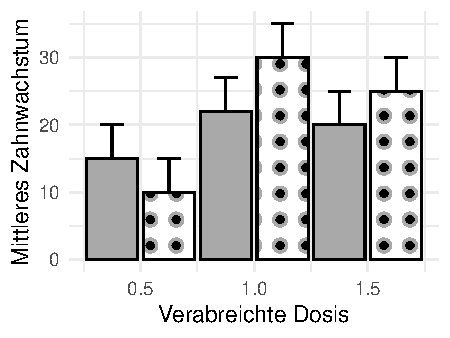
\includegraphics[width=\maxwidth]{img/mc-anova-02-a-1} 

}




Welche Aussage ist richtig im Bezug auf eine zweifaktorielle ANOVA?



\begin{enumerate}
\item [\textbf{A} \msquare] Keine Interaktion liegt vor. Die Geraden scheiden sich und laufen nicht parallel.
\item [\textbf{B} \msquare] Eine leichte Interaktion ist zu erwarten. Die Geraen schneiden sich noch nicht, aber die Abst{"a}nde unterscheiden sich stark.
\item [\textbf{C} \msquare] Eine starke Interaktion liegt vor. Die Geraden laufen parallel und schneiden sich nicht.
\item [\textbf{D} \msquare] Eine starke Interaktion ist zu erwarten. Die Geraden schneiden sich und die Abst{"a}nde sind nicht gleichbleibend.
\item [\textbf{E} \msquare] Keine Interaktion ist zu erwatzen. Die Geraden der Verabreichungsmethode laufen parallel und mit {"a}hnlichen Abst{"a}nden.
\end{enumerate} 
\section*{Deskriptive Statistik \& Explorative Datenanalyse}

\section{Aufgabe \hfill (2 Punkte)}




Berechnen Sie den Mittelwert und Standardabweichung von $y$ mit 5, 7, 11, 6 und 9.



\begin{enumerate}
\item [\textbf{A} \msquare] Es ergibt sich 7.6 +/- 5.8
\item [\textbf{B} \msquare] Es ergibt sich 6.6 +/- 2.9
\item [\textbf{C} \msquare] Es ergibt sich 7.6 +/- 1.205
\item [\textbf{D} \msquare] Es ergibt sich 8.6 +/- 1.205
\item [\textbf{E} \msquare] Es ergibt sich 7.6 +/- 2.41
\end{enumerate} 

\section{Aufgabe \hfill (2 Punkte)}




Berechnen Sie den Median, das $1^{st}$ Quartile sowie das $3^{rd}$ Quartile von $y$ mit 23, 15, 10, 10, 15, 18 und 51.



\begin{enumerate}
\item [\textbf{A} \msquare] Es ergibt sich 20 [11, 24]
\item [\textbf{B} \msquare] Es ergibt sich 15 +/- 10
\item [\textbf{C} \msquare] Es ergibt sich 15 [10, 23]
\item [\textbf{D} \msquare] Es ergibt sich 15 +/- 23
\item [\textbf{E} \msquare] Es ergibt sich 20 +/- 10
\end{enumerate} 

\section{Aufgabe \hfill (2 Punkte)}



Die empfohlene Mindestanzahl an Beobachtungen f{\"u}r ein Histogramm sind...



\begin{enumerate}
\item [\textbf{A} \msquare] 1 Beobachtung.
\item [\textbf{B} \msquare] 5 und mehr Beobachtungen.
\item [\textbf{C} \msquare] 10 Beobachtungen.
\item [\textbf{D} \msquare] 2-5 Beobachtungen.
\item [\textbf{E} \msquare] mindestens 20 Beobachtungen.
\end{enumerate} 

\section{Aufgabe \hfill (2 Punkte)}



Sie wollen nach einem Feldversuch die Varianz berechnen. Welche der folgenden Rechenoperationen m{"u}ssen durchgef{"u}hrt werden?



\begin{enumerate}
\item [\textbf{A} \msquare] Den Mittelwert berechen, dann die quadratischen Abst{"a}nde zum Mittelwert aufsummieren und durch die Fallzahl teilen.
\item [\textbf{B} \msquare] Den Mittelwert berechen, dann die absoluten Abst{"a}nde zum Mittelwert aufsummieren
\item [\textbf{C} \msquare] Den Mittelwert berechen, dann die quadratischen Abst{"a}nde zum Mittelwert aufsummieren und durch die Fallzahl teilen, dann die Wurzel ziehen.
\item [\textbf{D} \msquare] Den Mittelwert berechnen und die Abst{"a}nde quadrieren. Die Summe mit der Fallzahl multiplizieren.
\item [\textbf{E} \msquare] Den Median berechen, dann die quadratischen Abst{"a}nde zum Median aufsummieren, dann die Wurzel ziehen.
\end{enumerate}

\section{Aufgabe \hfill (2 Punkte)}



Der Barplot stellt folgende statistische Ma{\ss}zahlen in einer
Abbildung dar. Damit geh{\"o}rt der Barplot zu einem der am meisten
genutzten statistischen Verfahren zur Visualisierung von Daten. 



\begin{enumerate}
\item [\textbf{A} \msquare] Den Mittelwert und die Varianz.
\item [\textbf{B} \msquare] Den Mittelwert und die Standardabweichung.
\item [\textbf{C} \msquare] Den Median und die Standardabweichung.
\item [\textbf{D} \msquare] Den Mittelwert sowie den Median und die Streuung.
\item [\textbf{E} \msquare] Den Median und die Quartile.
\end{enumerate} 

\section{Aufgabe \hfill (2 Punkte)}



Nachdem Sie in einem Feldexperiment zu Leistungssteigerung von
Brokoli durchgef{\"u}hrt haben, berechnen Sie den Mittelwert und den
Median. Der Mittelwert $\bar{y}$ und der Median $\tilde{y}$
unterscheiden sich. Welche Aussage ist richtig?




\begin{enumerate}
\item [\textbf{A} \msquare] Da sich der Mittelwert und der Median unterscheiden, ist der Datensatz nicht zu verwenden. Mittelwert und Median m{"u}ssen gleich sein.
\item [\textbf{B} \msquare] Da sich der Mittelwert und der Median nicht unterscheiden, liegen vermutlich Outlier in den Daten vor.
\item [\textbf{C} \msquare] Da sich der Mittelwert und der Median unterscheiden, liegen vermutlich Outlier in den Daten vor. Wir untersuchen den Datensatz nach auff{"a}lligen Beobachtungen.
\item [\textbf{D} \msquare] Da sich der Mittelwert und der Median unterscheiden, liegen vermutlich keine Outlier in den Daten vor.
\item [\textbf{E} \msquare] Da sich der Mittelwert und der Median nicht unterscheiden, liegen vermutlich keine Outlier in den Daten vor. Wir verweden den Datensatz so wie er ist.
\end{enumerate}

\section{Aufgabe \hfill (2 Punkte)}



Um zu {\"U}berpr{\"u}fen, ob die Daten die Annahme einer Varianzhomogenit{"a}t gen{\"u}gen, k{\"o}nnen
wir folgende Visualisierung nutzen. Dabei kommt dann auch die entsprechende
Regel zur Absch{\"a}tzung der Annahme einer Varianzhomogenit{"a}t zur Anwendung. 



\begin{enumerate}
\item [\textbf{A} \msquare] Einen Barplot. Die Mittelwerte m{"u}ssen alle auf einer H{"o}he liegen. Die Fehlerbalken haben hier keine Informationen.
\item [\textbf{B} \msquare] Einen Boxplot. Das IQR muss {"u}ber alle Behandlungen zusammen mit den Whiskers ungef{"a}hr gleich sein.
\item [\textbf{C} \msquare] Einen Violinplot. Der Bauch der Violine muss hierbei einen h{"o}hren Wert annehmen als der Steg der Violine. Dann kann die Annahme angenommen werden.
\item [\textbf{D} \msquare] Einen Dotplot. Die Punkte m{"u}ssen sich wie an einer Perlenschnurr audreihen. Eine Abweichung f{"u}hrt zur Ablehnung der Annahme.
\item [\textbf{E} \msquare] Einen Boxplot. Der Median als Linie, muss in der Mitte des IQR, dargestellt durch die Box, liegen.
\end{enumerate}

\section{Aufgabe \hfill (2 Punkte)}



In der Statistik m{\"u}ssen wir h{\"a}ufig {\"U}berpr{\"u}fen, ob unser Outcome einer
bestimmten Verteilung folgt. Meistens {\"U}berpr{\"u}fen wir, ob eine
Normalverteilung vorliegt. Folgende drei Abbildungen eigenen sich im
Besonderen f{\"u}r die {\"U}berpr{\"u}fung einer Verteilungsannahme an eine Variable.



\begin{enumerate}
\item [\textbf{A} \msquare] Histogramm, Densityplot, Dotplot
\item [\textbf{B} \msquare] Scatterplot, Mosaicplot, Boxplot
\item [\textbf{C} \msquare] Histogramm, Scatterplot, Boxplot
\item [\textbf{D} \msquare] Barplot, Mosaicplot, Violinplot
\item [\textbf{E} \msquare] Boxplot, Densityplot, Violinplot
\end{enumerate}

\section{Aufgabe \hfill (2 Punkte)}



In dem folgenden Histogramm von $n = 207$ Pflanzen ist welche
Verteilung mit welchen korrekten Verteilungsparametern dargestellt?



{\centering 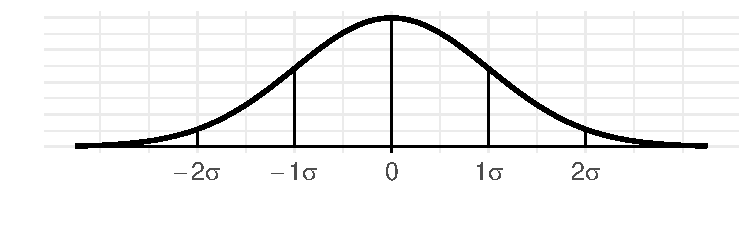
\includegraphics[width=\maxwidth]{img/mc-distribution-02-a-1} 

}







\begin{enumerate}
\item [\textbf{A} \msquare] Es handelt sich um eine Poisson-Verteilung mit Pois(20).
\item [\textbf{B} \msquare] Es handelt sich um eine Normalverteilung mit N(20, 5).
\item [\textbf{C} \msquare] Eine Standardnormalverteilung mit N(0,1).
\item [\textbf{D} \msquare] Es handelt sich um eine Binomial-Verteilung mit Binom(10).
\item [\textbf{E} \msquare] Eine rechtsschiefe, multivariate Normalverteilung.
\end{enumerate} 
\section*{Lineare Regression \& Korrelation}

\section{Aufgabe \hfill (2 Punkte)}




Sie haben das Modell $Y \sim X$ vorliegen und wollen nun ein
pr{"a}diktives Modell rechnen. Welche Aussage ist richtig?



\begin{enumerate}
\item [\textbf{A} \msquare] Ein pr{"a}diktives Modell ben{"o}tigt mindestens eine Fallzahl von {"u}ber 100 Beobachtungen und darf keine fehlenden Werte beinhalten. Die Varianzkomponenten m{"u}ssen homogen sein.
\item [\textbf{B} \msquare] Ein pr{"a}diktives Modell basiert auf einem Traingsdatensatz und einem Testdatensatz. Auf dem Trainingsdatensatz wird das Modell trainiert und auf dem Testdatensatz validiert.
\item [\textbf{C} \msquare] Ein pr{"a}diktives Modell m{"o}chte die Zusammenh{"a}nge von X auf Y modellieren. Hierbei geht es um die Effekte von X auf Y. Man sagt, wenn X um 1 ansteigt {"a}ndert sich Y um einen Betrag $\beta$.
\item [\textbf{D} \msquare] Ein pr{"a}diktives Modell schliesst grunds{"a}tzlich lineare Modell aus. Es muss ein Graph gefunden werden, der alle Punkte beinhaltet. Erst dann kann das $R^2$ berechnet werden.
\item [\textbf{E} \msquare] Ein pr{"a}diktives Modell wird auf einem Trainingsdatensatz trainiert und anschliessend {"u}ber eine explorative Datenanalyse validiert. Signifikanzen {"u}ber $\beta_i$ k{"o}nnen hier nicht festgestellt werden.
\end{enumerate} 

\section{Aufgabe \hfill (2 Punkte)}

Sie rechnen in eine linearen Regression und erhalten folgenden QQ
Plot. Welche Aussage ist richtig?




{\centering 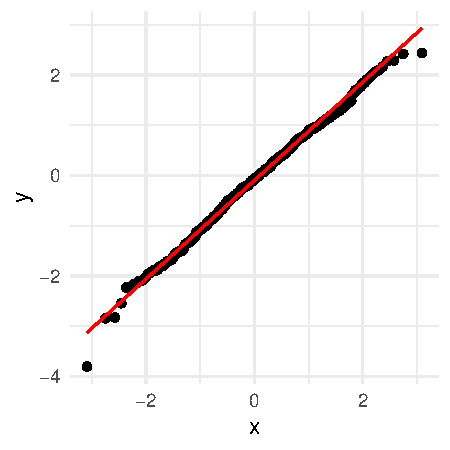
\includegraphics[width=\maxwidth]{img/mc-regression-05-a-1} 

}







\begin{enumerate}
\item [\textbf{A} \msquare] Die Annahme der normalverteilten Residuen ist erf{"u}llt. Die Punkte liegen zum {"u}berwiegenden Teil nicht auf der Geraden und Korrelation ist negativ.
\item [\textbf{B} \msquare] Die Annahme der normalverteilten Residuen ist erf{"u}llt. Die Punkte liegen zum {"u}berwiegenden Teil auf der Geraden.
\item [\textbf{C} \msquare] Die Annahme der normalverteilten Residuen ist nicht erf{"u}llt. Die Punkte liegen zum {"u}berwiegenden Teil nicht auf der Geraden.
\item [\textbf{D} \msquare] Die Annahme der normalverteilten Residuen ist erf{"u}llt. Die Punkte liegen zum {"u}berwiegenden Teil nicht auf der Geraden.
\item [\textbf{E} \msquare] Die Annahme der normalverteilten Residuen ist nicht erf{"u}llt. Die Punkte liegen zum {"u}berwiegenden Teil auf der Geraden.
\end{enumerate}

\section{Aufgabe \hfill (2 Punkte)}

Sie rechnen eine linearen Regression und erhalten folgenden Residual
Plot. Welche Aussage ist richtig?




{\centering 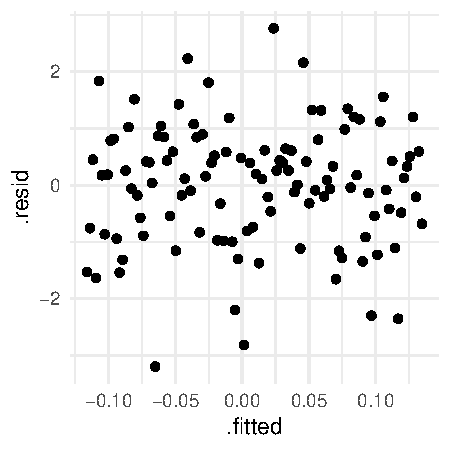
\includegraphics[width=\maxwidth]{img/mc-regression-06-a-1} 

}







\begin{enumerate}
\item [\textbf{A} \msquare] Die Annahme der normalverteilten Residuen ist erf{"u}llt. Es ist ein Muster zu erkennen.
\item [\textbf{B} \msquare] Die Annahme der normalverteilten Residuen ist nicht erf{"u}llt. Vereinzelte Punkte liegen oberhalb bzw. unterhalb der Geraden um die 0 Linie weiter entfernt. Ein klares Muster ist zu erkennen.
\item [\textbf{C} \msquare] Die Annahme der normalverteilten Residuen ist erf{"u}llt. Kein Muster ist zu erkennen und keine Outlier zu beobachten.
\item [\textbf{D} \msquare] Die Annahme der normalverteilten Residuen ist erf{"u}llt. Die Punkte liegen zum {"u}berwiegenden Teil auf der Diagonalen.
\item [\textbf{E} \msquare] Die Annahme der normalverteilten Residuen ist nicht erf{"u}llt. Es ist kein Muster zu erkennen.
\end{enumerate}

\section{Aufgabe \hfill (2 Punkte)}




Welche Aussage {\"u}ber den Korrelationskoeffizienten nach Spearman
ist richtig?



\begin{enumerate}
\item [\textbf{A} \msquare] Der Korrelationskoeffizienten nach Spearman wird genutzt, wenn der Korrelationskoeffizienten zwischen -1 und 1 liegt. Dann sind die Residuen normalverteilt.
\item [\textbf{B} \msquare] Der Korrelationskoeffizienten nach Spearman wird genutzt, wenn das Outcome Y nicht normalverteilt ist. Der Korrelationskoeffizienten liegt zwischen -1 und 1.
\item [\textbf{C} \msquare] Der Korrelationskoeffizienten nach Spearman wird genutzt, wenn das Outcome Y normalverteilt ist. Der Korrelationskoeffizienten liegt zwischen -1 und 1.
\item [\textbf{D} \msquare] Der Korrelationskoeffizienten nach Spearman wird genutzt, wenn das Outcome Y nicht normalverteilt ist. Der Korrelationskoeffizienten liegt zwischen 0 und 1.
\item [\textbf{E} \msquare] Der Korrelationskoeffizienten nach Spearman wird genutzt, wenn das Outcome Y normalverteilt ist. Der Korrelationskoeffizienten liegt zwischen 0 und 1.
\end{enumerate}

\section{Aufgabe \hfill (2 Punkte)}

Nach einer simplen linearen Regression zur Untersuchung vom Einfluss der
$CO_2$-Konzentration [$\mu g$] im Wasser auf das Wachstum von Wasserlinsen
[$kg$] erhalten Sie einen $\beta_1$ Koeffizienten von $0.00001$ und einen
hoch signifikanten $p$-Wert mit $2.3\cdot 10^{-9}$. Warum sehen Sie so einen kleinen
Effekt bei einer so deutlichen Signifikanz? 




\begin{enumerate}
\item [\textbf{A} \msquare] Die Einheit der $CO_2$-Konzentration ist zu klein gew{"a}hlt. Die Erh{"o}hung der $CO_2$-Konzentration um 1 f{"u}hrt nur zu einem sehr winzigen Anstieg im Gewicht der Wasserlinsen. Die Einheit muss besser gew{"a}hlt werden.
\item [\textbf{B} \msquare] Die Einheit der $CO_2$-Konzentration ist zu klein gew{"a}hlt. Dadurch sehen wir den sehr kleinen $p$-Wert. Der $p$-Wert und die Einheit von der $CO_2$-Konzentration h{"a}ngen zusammen.
\item [\textbf{C} \msquare] Die Fallzahl ist zu hoch angesetzt. Je h{"o}her die Fallzahl ist, desto kleiner ist die Teststatistik und damit ist dann auch der $p$-Wert sehr klein.
\item [\textbf{D} \msquare] Die Fallzahl ist zu klein angesetzt. Je kleiner die Fallzahl ist, desto h{"o}her ist die Teststatsitik und damit auch der $p$-Wert kleiner. 
\item [\textbf{E} \msquare] Das Gewicht und die $CO_2$-Konzentration korrelieren sehr stark, deshalb wird der $\beta_1$ Koeffizient sehr klein.
\end{enumerate}

\section{Aufgabe \hfill (2 Punkte)}

In einer linearen Regression werden die $\epsilon$ oder Residuen
gesch{\"a}tzt. Welcher Verteilung folgen die Residuen bei einer optimalen
Modellierung? 



\begin{enumerate}
\item [\textbf{A} \msquare] Die Residuen sind binomialverteilt.
\item [\textbf{B} \msquare] Die Residuen sind normalverteilt mit $\mathcal{N}(0, s^2)$.
\item [\textbf{C} \msquare] Die Residuen sind normalverteilt mit $\mathcal{N}(0, 1)$.
\item [\textbf{D} \msquare] Die Residuen folgen einer Poissonverteilung mit Pois(0).
\item [\textbf{E} \msquare] Die Residuen sind normalverteilt mit $\mathcal{N}(\bar{y}, s^2)$.
\end{enumerate}

\section{Aufgabe \hfill (2 Punkte)}

Welche Aussage {\"u}ber das \textit{generalisierte lineare Modell (GLM)} ist richtig?  



\begin{enumerate}
\item [\textbf{A} \msquare] Das GLM erlaubt auch nicht normalverteilte Residuen in der Sch{"a}tzung der Regressionsgrade.
\item [\textbf{B} \msquare] Das GLM ist eine allgemeine Erweiterung der linearen Regression auf die Normalverteilung.
\item [\textbf{C} \msquare] Das GLM ist eine Vereinfachung des LM in R. Mit dem GLM lassen polygonale Regressionen rechnen.
\item [\textbf{D} \msquare] Das GLM ist ein faktisch maschineller Lernalgorithmus, der selstst{"a}ndig die Verteilungsfamilie f{"u}r Y w{"a}hlt.
\item [\textbf{E} \msquare] Das GLM erlaubt auch weitere Verteilungsfamilien f{"u}r das Y bzw. das Outcome in einer linearen Regression zu w{"a}hlen.
\end{enumerate}
\section*{Vermischte Themen}  

\section{Aufgabe \hfill (2 Punkte)}




Welche Aussage {\"u}ber die parametrische Statistik ist richtig?



\begin{enumerate}
\item [\textbf{A} \msquare] Die parametrische Statistik basiert auf R{"a}ngen. Daher wird jeder Zahl ein Rang zugeteilt. Nur auf den R{"a}ngen wird die Auswertung gerechnet. Daher gibt es auch keinen direkt zu interpretierenden Effektsch{"a}tzer.
\item [\textbf{B} \msquare] Die parametrische Statistik basiert auf dem Sch{"a}tzen von Parametern aus einer festgelegten Verteilung. Daher gibt es auch direkt zu interpretierenden Effektsch{"a}tzer.
\item [\textbf{C} \msquare] Die parametrische Statistik basiert auf R{"a}ngen. Daher gibt es auch direkt zu interpretierenden Effektsch{"a}tzer.
\item [\textbf{D} \msquare] Die parametrische Statistik basiert auf dem Sch{"a}tzen von Parametern aus einer a priori festgelegten Verteilung. Daher gibt es auch direkt zu interpretierenden Effektsch{"a}tzer.
\item [\textbf{E} \msquare] Die nicht-parametrische Statistik ist ein Vorg{"a}nger der parametrischen Statistik und wurde wegen dem Mangel an Effektsch{"a}tzern nicht mehr ab 1960 genutzt.
\end{enumerate}

\section{Aufgabe \hfill (2 Punkte)}

Die Randomisierung von Beobachtungen bzw. Samples zu den Versuchseinheiten
ist bedeutend in der Versuchsplanung. Welche der folgenden Aussagen ist richtig?



\begin{enumerate}
\item [\textbf{A} \msquare] Randomisierung bringt starke Unstrukturiertheit in das Experiment und erlaubt erst von der Stichprobe auf die Grundgesamtheit zur{"u}ckzuschliessen.
\item [\textbf{B} \msquare] Randomisierung sorgt f{"u}r Strukturgleichheit und erlaubt erst von der Stichprobe auf die Grundgesamtheit zur{"u}ckzuschliessen.
\item [\textbf{C} \msquare] Randomisierung erlaubt erst die Varianzen zu sch{"a}tzen. Ohne eine Randomisierung ist die Berechnung von Mittelwerten und Varianzen nicht m{"o}glich.
\item [\textbf{D} \msquare] Randomisierung erlaubt erst die Mittelwerte zu sch{"a}tzen. Ohne Randomisierung keine Mittelwerte.
\item [\textbf{E} \msquare] Randomisierung war bis 1952 bedeutend, wurde dann aber in Folge besserer Rechnerleistung nicht mehr verwendet. Aktuelle Statistik nutzt keine Randomisierung mehr.
\end{enumerate}

\section{Aufgabe \hfill (2 Punkte)}

Wenn Sie einen Datensatz erstellen, dann ist es ratsam die Spalten und die
Eintr{\"a}ge in englischer Sprache zu verfassen, wenn Sie sp{\"a}ter die Daten in
\Rlogo auswerten wollen. Welcher folgende Grund ist richtig?



\begin{enumerate}
\item [\textbf{A} \msquare] Es gibt keinen Grund nicht auch deutsche W{"o}rter zu verwenden. Es ist ein Stilmittel.
\item [\textbf{B} \msquare] Programmiersprachen k{"o}nnen nur englische Begriffe verarbeiten. Zus{"a}tzliche Pakete k{"o}nnen zwar geladen werden, aber meist funktionieren diese Pakete nicht richtig. Deutsch ist International nicht bedeutend genug.
\item [\textbf{C} \msquare] Im Allgemeinen haben Programmiersprachen Probleme mit Umlauten und Sonderzeichen, die in der deutschen Sprache vorkommen. Eine Nutzung der englischen Sprache umgeht dieses Problem auf einfache Art.
\item [\textbf{D} \msquare] Alle Funktionen und auch Anwendungen sind in \Rlogo in englischer Sprache. Die Nutzung von deutschen W{"o}rtern ist nicht schick und das ist zu vermeiden.
\item [\textbf{E} \msquare] Die Spracherkennung von \Rlogo ist nicht in der Lage Deutsch zu verstehen.
\end{enumerate}

\section{Aufgabe \hfill (2 Punkte)}

Bei der explorativen Datenanalyse (EDA) in \Rlogo gibt es eine richtige Abfolge von Prozessschritten, auch \textit{Circle of life} genannt. Wie lautet die richtige Reihenfolge f{\"u}r die Erstellung einer EDA?



\begin{enumerate}
\item [\textbf{A} \msquare] Wir lesen die Daten ein und mutieren die Daten. Dabei ist wichtig, dass wir nicht das Paket \texttt{tidyverse} nutzen, da dieses Paket veraltet ist. {"U}ber die Funktion \texttt{library(tidyverse)} entfernen wir das Paket von der Analyse.
\item [\textbf{B} \msquare] Wir lesen die Daten {"u}ber eine generische Funktion \texttt{read()} ein und m{"u}ssen dann die Funktion \texttt{ggplot()} nur noch installieren. Dann haben wir die Abbildungen als \texttt{*.png} vorliegen.
\item [\textbf{C} \msquare] Wir lesen als erstes die Daten {"u}ber \texttt{read\_excel()} ein, transformieren die Spalten {"u}ber \texttt{mutate()} in die richtige Form und k{"o}nnen dann {"u}ber \text{ggplot()} uns die Abbildungen erstellen lassen.
\item [\textbf{D} \msquare] Wir transformieren die Spalten {"u}ber \texttt{mutate()} in ein \texttt{tibble} und k{"o}nnen dann {"u}ber \text{ggplot()} uns die Abbildungen erstellen lassen. Dabei beachten wir das wir keine Faktoren in den Daten haben.
\item [\textbf{E} \msquare] Wir lesen als erstes die Daten {"u}ber \texttt{read\_excel()} ein, transformieren die Spalten {"u}ber \texttt{mutate()} in die richtige Form und k{"o}nnen dann  {"u}ber \text{ggplot()} uns die Abbildungen erstellen lassen. Wichtig ist, dass wir keine Faktoren sondern nur numerische Variablen vorliegen haben.
\end{enumerate}

\section{Aufgabe \hfill (2 Punkte)}




Sie haben das abstrakte Modell $Y \sim X$ mit $X$ als Faktor mit zwei
Leveln vorliegen. Welche Aussage {\"u}ber $n_1 = n_2$ ist richtig?



\begin{enumerate}
\item [\textbf{A} \msquare] Es liegt Varianzhetrogenit{"a}t vor.
\item [\textbf{B} \msquare] Es handelt sich um ein balanciertes Design.
\item [\textbf{C} \msquare] Es handelt sich um ein unbalanciertes Design
\item [\textbf{D} \msquare] Es liegt Varianzhomogenit{"a}t vor.
\item [\textbf{E} \msquare] Es handelt sich um abh{"a}ngige Beobachtungen.
\end{enumerate}

\section{Aufgabe \hfill (2 Punkte)}

In einem Zuchtexperiment messen wir die Ferkel verschiedener Sauen. Die
Ferkel einer Muttersau sind daher im statistischen Sinne... 



\begin{enumerate}
\item [\textbf{A} \msquare] Untereinander unabh{"a}ngig. Sollten die M{"u}tter verwandt sein, so ist die Varianzstruktur {"a}hnlich und muss modelliert werden.
\item [\textbf{B} \msquare] Untereinander stark korreliert. Die Ferkel sind von einer Mutter und sommit miteinander korreliert. Dies wird in der Statistik jedoch meist nicht modelliert.
\item [\textbf{C} \msquare] Untereinander unabh{"a}ngig. Die Ferkel sind eigenst{"a}ndig und ben{"o}tigen keine zus{"a}tzliche Behandlung.
\item [\textbf{D} \msquare] Untereinander abh{"a}ngig. Die Ferkel stammen von einem Muttertier und haben vermutliche eine {"a}hnliche Varianzstruktur.
\item [\textbf{E} \msquare] Untereinander abh{"a}ngig, wenn die M{"u}tter ebenfalls miteinander verwandt sind. Erst die Abh{"a}ngigkeit 2. Grades wird in der Statistik modelliert.
\end{enumerate}

\section{Aufgabe \hfill (2 Punkte)}



Sie f{\"u}hren ein Experiment zur Behandlung von Klaueninfektionen bei K{\"u}hen
durch. Bei 6 Tieren finden Sie eine Erkrankung der Klauen vor und
7 Tiere sind gesund. Welche Aussage {\"u}ber den Odds ratio
Effektsch{\"a}tzer ist richtig?



\begin{enumerate}
\item [\textbf{A} \msquare] Es ergibt sich ein Odds ratio von 0.46, da es sich um ein Anteil handelt.
\item [\textbf{B} \msquare] Es ergibt sich ein Odds ratio von 0.86, da es sich um ein Anteil handelt.
\item [\textbf{C} \msquare] Es ergibt sich ein Odds ratio von 0.46, da es sich um eine Chancenverh{"a}ltnis handelt.
\item [\textbf{D} \msquare] Es ergibt sich ein Odds ratio von 1.17, da es sich um ein Anteil handelt.
\item [\textbf{E} \msquare] Es ergibt sich ein Odds ratio von 0.86, da es sich um eine Chancenverh{"a}ltnis handelt.
\end{enumerate}

\section{Aufgabe \hfill (2 Punkte)}

In der Bio Data Science wird h{\"a}ufig mit sehr gro{\ss}en Datens{\"a}tzen
gerechnet. Historisch ergibt sich nun ein Problem bei der Auswertung der
Daten und deren Bewertung hinsichtlich der Signifikanz. Welche Aussage ist richtig?



\begin{enumerate}
\item [\textbf{A} \msquare] Aktuell werden immer gr{"o}ssere Datens{"a}tze erhoben. Eine erh{"o}hte Fallzahl f{"u}hrt automatisch auch zu mehr signifikanten Ergebnissen, selbst wenn die eigentlichen Effekte nicht relevant sind.
\item [\textbf{B} \msquare] Aktuell werden zu grosse Datens{"a}tze f{"u}r die g{"a}nigige Statistik gemessen. Daher wendet man maschinelle Lernverfahren f{"u}r kausale Modelle an. Hier ist die Relevanz gleich Signifikanz.
\item [\textbf{C} \msquare] Big Data ist ein Problem der parametrischen Statistik. Parameter lassen sich nur auf kleinen Datens{"a}tzen berechnen, da es sich sonst nicht mehr um eine Stichprobe im engen Sinne der Statistik handelt.
\item [\textbf{D} \msquare] Relevanz und Signifikanz haben nichts miteinander zu tun. Daher gibt es auch keinen Zusammenhang zwischen hoher Fahlzahl (n > 10000) und einem signifikanten Test. Ein Effekt ist immer relevant und somit signifikant.
\item [\textbf{E} \msquare] Aktuell werden immer gr{"o}ssere Datens{"a}tze erhoben. Dadurch wird auch die Varianz immer h{"o}her was automatisch zu mehr signifikanten Ergebnissen f{"u}hrt.
\end{enumerate}
\section*{Multiple Gruppenvergleiche}    

\section{Aufgabe \hfill (2 Punkte)}



Sie haben folgende unadjustierten p-Werte gegeben: 0.02, 0.34, 0.001, 0.01 und 0.89. Sie adjustieren die p-Werte nach
Bonferroni. Welche Aussage ist richtig?



\begin{enumerate}
\item [\textbf{A} \msquare] Nach der Bonferroni-Adjustierung ergeben sich die adjustierten p-Werte von 0.004, 0.068, 2e-04, 0.002 und 0.178. Die adjustierten p-Werte werden zu einem $\alpha$-Niveau von 5\% verglichen.
\item [\textbf{B} \msquare] Nach der Bonferroni-Adjustierung ergeben sich die adjustierten p-Werte von 0.1, 1.7, 0.005, 0.05 und 4.45. Die adjustierten p-Werte werden zu einem $\alpha$-Niveau von 5\% verglichen.
\item [\textbf{C} \msquare] Nach der Bonferroni-Adjustierung ergeben sich die adjustierten p-Werte von 0.1, 1, 0.005, 0.05 und 1. Die adjustierten p-Werte werden zu einem $\alpha$-Niveau von 5\% verglichen.
\item [\textbf{D} \msquare] Nach der Bonferroni-Adjustierung ergeben sich die adjustierten p-Werte von 0.1, 1, 0.005, 0.05 und 1. Die adjustierten p-Werte werden zu einem $\alpha$-Niveau von 1\% verglichen.
\item [\textbf{E} \msquare] Nach der Bonferroni-Adjustierung ergeben sich die adjustierten p-Werte von 0.004, 0.068, 2e-04, 0.002 und 0.178. Die adjustierten p-Werte werden zu einem $\alpha$-Niveau von 1\% verglichen.
\end{enumerate}

\section{Aufgabe \hfill (2 Punkte)}

Die Abk{\"u}rzung \textit{CLD} steht f{\"u}r welches statistische Verfahren? Welche
anschlie{\ss}ende Beschreibung der Interpretation ist korrekt? 



\begin{enumerate}
\item [\textbf{A} \msquare] Contrast letter display. Unterschiede in den Behandlungen werden durch den gleichen Buchstaben oder Symbol dargestellt. Die Interpretation des CLD f{"u}hrt h{"a}ufig in die Irre.
\item [\textbf{B} \msquare] Compact line display. Gleichheit in den Behandlungen wird durch den gleichen Buchstaben oder Symbol dargestellt. Fr{"u}her wurden keine Buchstaben sondern eine durchgezogene Linie verwendet. Bei mehr als drei Gruppen funktioniert die Linie aber graphisch nicht mehr.
\item [\textbf{C} \msquare] Compact letter display. Gleichheit in den Behandlungen wird durch den gleichen Buchstaben oder Symbol dargestellt. Teilweise ist die Interpretation des CLD herausfordernd, da wir ja nach dem Unterschied suchen.
\item [\textbf{D} \msquare] Compound letter display. Gleichheit in dem Outcomes wird durch den gleichen Buchstaben oder Symbol dargestellt. Teilweise ist die Interpretation des Verbunds (eng. compound) herausfordernd, da wir ja nach dem Unterschied suchen.
\item [\textbf{E} \msquare] Compact letter detection. Gleichheit in den Behandlungen wird durch den gleichen Buchstaben oder Symbol dargestellt.
\end{enumerate}

\section{Aufgabe \hfill (2 Punkte)}

Der multiple Vergleich als Posthoc-Test nach einer ANOVA ist in den
Agrarwissenschaften heutzutage Standard. Welches R Paket wird h{\"a}ufig f{\"u}r
den multiplen Vergleich genutzt? Welche Beschreibung der Eigenschaften ist korrekt?



\begin{enumerate}
\item [\textbf{A} \msquare] Das R Paket lm. Das Paket lm erstellt selbstst{"a}ndig Konfidenzintervalle und entsprechende p-Werte. Da wir in dem Paket nicht adjustieren m{"u}ssen, ist es bei Anwendern sehr beliebt.
\item [\textbf{B} \msquare] Das R Paket emmeans erlaubt die Durchf{"u}hrung eines multiplen Gruppenvergleichs. Aus einem emmeans Objekt l{"a}sst sich recht einfach das CLD erstellen und so {"u}ber Barplots eine schnelle Interpration der statistischen Auswertung durchf{"u}hren.
\item [\textbf{C} \msquare] Das R Paket emmeans erlaubt die Durchf{"u}hrung eines multiplen Gruppenvergleichs. Aus einem emmeans Objekt l{"a}sst sich leider kein CLD erstellen. Dennoch ist das Paket einfach zu bedienen und wird deshalb genutzt. Die Interpretation der statistischen Auswertung wird {"u}ber einen Barplot abgebildet.
\item [\textbf{D} \msquare] Das R Paket hmisc erlaubt die Durchf{"u}hrung eines multiplen Gruppenvergleichs aus verschiedenen Modellen heraus. Aus einem hmisc Objekt l{"a}sst sich recht einfach das CL-h erstellen und so {"u}ber Barplots eine schnelle Interpration der statistischen Auswertung durchf{"u}hren.
\item [\textbf{E} \msquare] Das R Paket ggplot. Wir erhalten hier sofort eine Visualisierung der Daten. Anhand der Visualisierung l{"a}sst sich eine explorative Datenanalyse durchf{"u}hren, die gleichwertig zu einem Posthoc-Test ist.
\end{enumerate}

\section{Aufgabe \hfill (2 Punkte)}

Bei einem multiplen Vergleich oder Posthoc Test kann es zu einer Besonderheit beim
statistischen Testen kommen. Wie nennt man diese Besonderheit beim
statistischen Testen und wie kann man mit ihr umgehen?



\begin{enumerate}
\item [\textbf{A} \msquare] Beim multiplen Testen kann es zu einer $\alpha$-Deflation kommen. Das globale Signifikanzniveau liegt nicht mehr bei $5\%$ sondern weit darunter. Daher m{"u}ssen die p-Werte entsprechend adjustiert werden. Hierf{"u}r gibt es verschiedene Verfahren, wobei das Verfahren zur Adjustierung der p-Werte nach Bonferroni das bekanneste Verfahren ist. Die p-Werte werden durch die Anzahl an Vergleichen geteilt
\item [\textbf{B} \msquare] Beim multiplen Testen kann es zu einer $\alpha$-Inflation kommen. Das globale Signifikanzniveau liegt nicht mehr bei $5\%$ sondern weit darunter. Daher m{"u}ssen die p-Werte entsprechend adjustiert werden. Hierf{"u}r gibt es verschiedene Verfahren, wobei das Verfahren zur Adjustierung der p-Werte nach Welch das bekanneste Verfahren ist.
\item [\textbf{C} \msquare] Beim multiplen Testen kann es zu einer $\alpha$-Inflation kommen. Das globale Signifikanzniveau liegt nicht mehr bei $5\%$ sondern sehr viel h{"o}her. Daher m{"u}ssen die p-Werte entsprechend adjustiert werden. Hierf{"u}r gibt es verschiedene Verfahren, wobei das Verfahren zur Adjustierung der p-Werte nach Bonferroni das bekanneste Verfahren ist.
\item [\textbf{D} \msquare] Beim multiplen Testen kann es zu einer $\beta$-Inflation kommen. Das globale Signifikanzniveau liegt nicht mehr bei $20\%$. Daher m{"u}ssen die p-Werte entsprechend adjustiert werden. Hierf{"u}r gibt es verschiedene Verfahren, wobei das Verfahren zur Adjustierung der p-Werte nach Bonferroni das bekanneste Verfahren ist.
\item [\textbf{E} \msquare] Beim multiplen Testen kann es zu Varianzheterogenit{"a}t kommen. Das globale Signifikanzniveau liegt nicht mehr bei $5\%$. Daher m{"u}ssen die p-Werte entsprechend adjustiert werden. Das Verfahren nach Welch, bekannt aus dem t-Test, ist hier h{"a}ufig anzuwenden.
\end{enumerate}
\section*{Statistische Testtheorie}  

\section{Aufgabe \hfill (2 Punkte)}

Welche Aussage zum mathematische Ausdruck $Pr(D|H_0)$ ist richtig? 



\begin{enumerate}
\item [\textbf{A} \msquare] $Pr(D|H_0)$ ist die Wahrscheinlichkeit der Alternativehypothese und somit $1 - Pr(H_A)$
\item [\textbf{B} \msquare] Die Inverse der Wahrscheinlichkeit unter der die Nullhypothese nicht mehr die Alternativehypothese {"u}berdeckt.
\item [\textbf{C} \msquare] $Pr(D|H_0)$ ist die Wahrscheinlichkeit die Daten D zu beobachten wenn die Nullhypothese wahr ist.
\item [\textbf{D} \msquare] Die Wahrscheinlichkeit f{"u}r die Nullhypothese, wenn die Daten wahr sind.
\item [\textbf{E} \msquare] Die Wahrscheinlichkeit der Daten unter der Nullhypothese in der Grundgesamtheit.
\end{enumerate}

\section{Aufgabe \hfill (2 Punkte)}



Das statistische Testen basiert auf dem Falsifikationsprinzip. Es besagt,



\begin{enumerate}
\item [\textbf{A} \msquare] ... dass ein schlechtes Modell durch ein weniger schlechtes Modell ersetzt wird. Die Wissenschaft lehnt ab und verifiziert nicht.
\item [\textbf{B} \msquare] ... dass Modelle meist falsch sind und selten richtig.
\item [\textbf{C} \msquare] ... dass in der Wissenschaft immer etwas falsch sein muss. Sonst gebe es keinen Fortschritt.
\item [\textbf{D} \msquare] ... dass Annahmen an statistische Modelle meist falsch sind.
\item [\textbf{E} \msquare] ... dass Fehlerterme in statistischen Modellen nicht verifiziert werden k{"o}nnen.
\end{enumerate}

\section{Aufgabe \hfill (2 Punkte)}

Der Fehler 1. Art oder auch Signifikanzniveau $\alpha$ genannt, liegt bei
5\%. Welcher der folgenden Gr{\"u}nde f{\"u}r diese Festlegeung auf 5\% ist richtig?



\begin{enumerate}
\item [\textbf{A} \msquare] Der Begr{"u}nder der modernen Statistik, R. Fischer, hat die Grenze simuliert und berechnet. Dadurch ergibt sich dieser optimale Cut-Off.
\item [\textbf{B} \msquare] Im Rahmen eines langen Disputs zwischen Neyman und Fischer wurde $\alpha = 5\%$ festgelegt. Leider werden die Randbedingungen und Voraussetzungen an statistsiche Modelle heute immer wieder ignoriert.
\item [\textbf{C} \msquare] Der Wert ergab sich aus einer Auswertung von 1042 wissenschaftlichen Ver{"o}ffentlichungen zwischen 1914 und 1948. Der Wert $5\%$ wurde in $28\%$ der Ver{"o}ffentlichungen genutzt. Daher legte man sich auf diese Zahl fest.
\item [\textbf{D} \msquare] Die Festlegung von $\alpha = 5\%$ ist eine Kulturkonstante. Wissenschaftler ben{"o}tigt eine Schwelle f{"u}r eine statistische Testentscheidung, der Wert von $\alpha$ wurde aber historisch mehr zuf{"a}llig gew{"a}hlt.
\item [\textbf{E} \msquare] Auf einer Statistikkonferenz in Genf im Jahre 1942 wurde dieser Cut-Off nach langen Diskussionen festgelegt. Bis heute ist der Cut Off aber umstritten, da wegen dem 2. Weltkrieg viele Wissenschaftler nicht teilnehmen konnten.
\end{enumerate}

\section{Aufgabe \hfill (2 Punkte)}

Betrachten wir die Teststatistik aus einem abstrakteren Blickwinkel. Beim
statistischen Testen wird das \textit{"`signal"'} mit dem
\textit{"`noise"'} zu einer Teststatistik T verrechnet. Welche der Formel
berechnet korrekt die Teststatistik T?



\begin{enumerate}
\item [\textbf{A} \msquare] Es gilt $T = \cfrac{signal}{noise}$
\item [\textbf{B} \msquare] Es gilt $T = signal \cdot noise$
\item [\textbf{C} \msquare] Es gilt $T = \cfrac{signal}{noise^2}$
\item [\textbf{D} \msquare] Es gilt $T = \cfrac{noise}{signal}$
\item [\textbf{E} \msquare] Es gilt $T = (signal \cdot noise)^2$
\end{enumerate}

%% ------------------------------------------------------------

\section{Aufgabe \hfill (2 Punkte)}



In der Theorie zur statistischen Testentscheidung kann "`$H_0$ beibehalten obwohl die $H_0$ falsch ist"'
in welche richtige Analogie gesetzt werden?



\begin{enumerate}
\item [\textbf{A} \msquare] In die Analogie eines Rauchmelders: \textit{Alarm with fire}.
\item [\textbf{B} \msquare] In die Analogie eines Rauchmelders: \textit{Fire without alarm}, dem $\beta$-Fehler.
\item [\textbf{C} \msquare] In die Analogie eines brennenden Hauses ohne Rauchmelder: \textit{House without noise}.
\item [\textbf{D} \msquare] In die Analogie eines Feuerwehrautos: \textit{Car without noise}.
\item [\textbf{E} \msquare] In die Analogie eines Rauchmelders: \textit{Alarm without fire}, dem $\alpha$-Fehler.
\end{enumerate}

\section{Aufgabe \hfill (2 Punkte)}

Welche statistische Masszahl erlaubt es \textit{Relevanz} mit
\textit{Signifikanz} zuverbinden? Welche Aussage ist richtig?



\begin{enumerate}
\item [\textbf{A} \msquare] Die Teststatistik. Durch den Vergleich von $T_c$ zu $T_k$ ist es m{"o}glich die $H_0$ abzulehnen. Die Relevanz ergibt sich aus der Fl{"a}che rechts vom dem $T_c$-Wert.
\item [\textbf{B} \msquare] Der p-Wert. Durch den Vergleich mit $\alpha$ l{"a}sst sich {"u}ber die Signifikanz entscheiden und der $\beta$-Fehler erlaubt {"u}ber die Power eine Einsch{"a}tzung der Relevanz.
\item [\textbf{C} \msquare] Das Konfidenzintervall. Durch die Visualizierung des Konfidenzintervals kann eine Relevanzschwelle vom Anwender definiert werden. Zus{"a}tzlich erlaubt das Konfidenzinterval auch eine Entscheidung {"u}ber die Signifikanz.
\item [\textbf{D} \msquare] Das OR. Als Chancenverh{"a}ltnis gibt es das Verh{"a}ltnis von Relevanz und Signifikanz wieder.
\item [\textbf{E} \msquare] Das $\Delta$. Durch die Effektst{"a}rke haben wir einen Wert f{"u}r die Relevanz, die vom Anwender bewertet werden muss. Da $\Delta$ antiproportional zum p-Wert ist, bedeutet auch ein hohes $\Delta$ ein sehr kleinen p-Wert.
\end{enumerate}

\section{Aufgabe \hfill (2 Punkte)}

Welche Aussage über den $p$-Wert und dem Signifikanzniveau $\alpha$ gleich 5\% ist richtig?



\begin{enumerate}
\item [\textbf{A} \msquare] Wir vergleichen die Effekte des $p$-Wertes mit den Effekten der Signifiaknzschwelle unter der Annahme der Nullhypothese.
\item [\textbf{B} \msquare] Wir vergleichen mit dem $p$-Wert und dem Signifikanzniveau $\alpha$ absolute Werte auf einem Zahlenstrahl und damit den Unterschied der Teststatistiken, wenn die $H_0$ gilt.
\item [\textbf{C} \msquare] Wir machen eine Aussage über die indivduelle Wahrscheinlichkeit des Eintretens der Nullhypothese $H_0$.
\item [\textbf{D} \msquare] Wir vergleichen mit dem $p$-Wert und dem Signifikanzniveau $\alpha$ Wahrscheinlichkeiten und damit die absoluten Werte auf einem Zahlenstrahl, wenn die $H_0$ gilt.
\item [\textbf{E} \msquare] Wir vergleichen mit dem $p$-Wert und dem Signifikanzniveau $\alpha$ Wahrscheinlichkeiten und damit die Flächen unter der Kurve der Teststatistik, wenn die $H_0$ gilt.
\end{enumerate}

\section{Aufgabe \hfill (2 Punkte)}



Die Ergebnisse der einer statistischen Analyse k{\"o}nnen in die Analogie einer
Wettervorhersage gebracht werden. Welche Analogie f{\"u}r die
Ergebnisse eines statistischen Tests trifft am besten zu?



\begin{enumerate}
\item [\textbf{A} \msquare] In der Analogie der Regenwahrscheinlichkeit: ein statistischer Test gibt die Wahrscheinlichkeit f{"u}r das Auftreten eines Ereignisses wieder. Die St{"a}rke des Effektes wird nicht wiedergeben.
\item [\textbf{B} \msquare] In der Analogie des Niederschlags oder Regenmenge: ein statistischer Test gibt die St{"a}rke eines Effektes wieder. Zum Beispiel, wie hoch ist der Mittelwertsunterschied.
\item [\textbf{C} \msquare] In der Analogie der Sonnenscheindauer: Wie lange kann mit einem entsprechenden Effekt gerechnet werden? Die Wahrscheinlichkeit f{"u}r den Effekt gibt der statistische Test wieder.
\item [\textbf{D} \msquare] In der Analogie der Maximaltemperatur: Was ist der maximale Unterschied zwischen zwei Gruppen. Wir erhalten hier eine Aussage {"u}ber die Spannweite und den maximalen Effekt.
\item [\textbf{E} \msquare] In der Analogie der Durchschnittstemperatur: Wie oft tritt ein Effekt durchschnittlich ein? Wir erhalten eine Wahrscheinlichkeit f{"u}r die Effekte. Zum Beispiel, wie hoch ist die Wahrscheinlichkeit f{"u}r einen Mittelwert als Durchschnitt.
\end{enumerate}

\section{Aufgabe \hfill (2 Punkte)}



Sie wollen eine Aussage {\"u}ber ein untersuchtes Individuum treffen. Dazu nutzen Sie einen
statistischen Test. K{\"o}nnen Sie eine valide Aussage zum Individuum
aus einem statistischen Test erhalten? 



\begin{enumerate}
\item [\textbf{A} \msquare] Ja, ein untersuchtes Individuum k{"o}nnen wir mit einem statistischen Test auswerten. Wir erhalten eine Aussage zum Individuum.
\item [\textbf{B} \msquare] Weder eine Ausssage {"u}ber die Population noch {"u}ber das Individuum ist mit einem statistischen Test m{"o}glich. Wir erhalten eine Aussage {"u}ber ein Experiment.
\item [\textbf{C} \msquare] Ja, wir erhalten eine Aussage. M{"u}ssen aber das Individuum im Kontext der Population adjustieren.
\item [\textbf{D} \msquare] Nein, ein untersuchtes Individuum k{"o}nnen wir mit einem statistischen Test nicht auswerten. Wir erhalten keine Aussage zum Individuum.
\item [\textbf{E} \msquare] Nein, wir erhalten nur eine Aussage zu zwei Individuen. Ein statistischer Test liefert Informationen zu einem Individuum im Vergleich zu einem anderen Individuum.
\end{enumerate}

\section{Aufgabe \hfill (2 Punkte)}

Welche Aussage {\"u}ber die Power ist richtig?



\begin{enumerate}
\item [\textbf{A} \msquare] Die Power $1-\beta$ wird auf 80\% gesetzt. Damit liegt die Wahrscheinlichkeit f{"u}r die $H_0$ bei 20\%.
\item [\textbf{B} \msquare] Die Power beschreibt die Wahrscheinlichkeit die $H_A$ abzulehnen. Wir testen die Power jedoch nicht.
\item [\textbf{C} \msquare] Die Power $1-\beta$ wird auf 80\% gesetzt. Alle statistischen Tests sind so konstruiert, dass die $H_A$ mit 80\% "bewiesen wird".
\item [\textbf{D} \msquare] Die Power ist nicht in der aktuellen Testthorie mehr vertreten. Wir rechnen nur noch mit dem Fehler 1. Art.
\item [\textbf{E} \msquare] Es gilt $\alpha + \beta = 1$ und somit liegt $\beta$ meist bei 95\%.
\end{enumerate}
\section*{Statistische Tests für Gruppenvergleiche} 

\section{Aufgabe \hfill (2 Punkte)}

Welche Aussage {\"u}ber den t-Test im Allgmeinen ist richtig? 



\begin{enumerate}
\item [\textbf{A} \msquare] Der t-Test vergleicht die Varianzen von mindestens zwei oder mehr Gruppen
\item [\textbf{B} \msquare] Der t-Test vergleicht die Mittelwerte von zwei Gruppen.
\item [\textbf{C} \msquare] Der t-Test testet generell zu einem erh{"o}hten $\alpha$-Niveau von 20\%.
\item [\textbf{D} \msquare] Der t-Test ist ein Vortest der ANOVA und basiert daher auf dem Vergleich von Streuungsparametern
\item [\textbf{E} \msquare] Der t-Test vergleicht die Mittelwerte von zwei Gruppen unter der strikten Annahme von Varianzhomogenit{"a}t. Sollte keine Varianzhomogenit{"a}t vorliegen, so gibt es keine M{"o}glichkeit den t-Test in einer Variante anzuwenden.
\end{enumerate}

\section{Aufgabe \hfill (2 Punkte)}

Welche Aussage {\"u}ber den Welch t-Test ist richtig?



\begin{enumerate}
\item [\textbf{A} \msquare] Der Welch t-Test vergleicht die Varianz von zwei Gruppen.
\item [\textbf{B} \msquare] Der Welch t-Test wird angewendet, wenn Varianzheterogenit{"a}t zwischen den beiden zu vergleichenden Gruppen vorliegt.
\item [\textbf{C} \msquare] Der Welch t-Test vergleicht die Mittelwerte von zwei Gruppen unter der strikten Annahme von Varianzhomogenit{"a}t.
\item [\textbf{D} \msquare] Der Welch t-Test ist die veraltete Form des Student t-Test und wird somit nicht mehr verwendet.
\item [\textbf{E} \msquare] Der Welch t-Test ist ein Post-hoc Test der ANOVA und basiert daher auf dem Vergleich der Varianz.
\end{enumerate}

\section{Aufgabe \hfill (2 Punkte)}

Welche Aussage {\"u}ber den gepaarten t-Test f{\"u}r verbundene Stichproben ist richtig?



\begin{enumerate}
\item [\textbf{A} \msquare] Der gepaarte t-Test wird genutzt, wenn die Differenzen der Beobachtungen verbunden sind und wir dadurch die Unabh{"a}{"a}ngigkeit nicht mehr vorliegen haben.
\item [\textbf{B} \msquare] Der gepaarte t-Test wird gerechnet, wenn die Beobachtungen abh{"a}ngig voneinander sind. Wir messen jede Beobachtung nur einmal und berechnen dann die Differenz zu dem Mittel der anderen Beobachtungen.
\item [\textbf{C} \msquare] Der gepaarte t-Test nutzt die Varianz der Beobachtungen jeweils paarweise und bildet daf{"u}r eine verbundene Stichprobe. Dieser Datensatz $d$ dient dann zur Differenzbildung.
\item [\textbf{D} \msquare] Beim gepaarten t-Test kombinieren wir die Vorteile des Student t-Test f{"u}r Varianzhomogenit{"a}t mit den Vorteilen des Welch t-Test f{"u}r Varianzheterogenit{"a}t. Wir bilden daf{"u}r die Differenz der Einzelbeobachtungen.
\item [\textbf{E} \msquare] Der gepaarte t-Test wird gerechnet, wenn die Beobachtungen nicht unabh{"a}ngig voneinander sind. Wir messen wiederholt an dem gleichen Probanden oder Tier oder Pflanze. Wir bilden die Differenzen um den gepaarten t-Test rechnen zu k{"o}nnen.
\end{enumerate}

\section{Aufgabe \hfill (2 Punkte)}

Nach einem Experiment mit f{\"u}nf Weizensorten ergibt eine ANOVA ($p = 0.041$)
einen signifikanten Unterschied f{\"u}r den Ertrag. Sie f{\"u}hren anschlie{\ss}end die
paarweisen t-Tests f{\"u}r alle Vergleiche der verschiedenen Weizensorten
durch. Nach der Adjustierung f{\"u}r multiples Testen ist kein p-Wert unter der
$\alpha$-Schwelle. Sie schauen sich auch die rohen, unadjustierten p-Werte
an und finden hier als niedrigsten p-Wert $p_{3-2} = 0.053$. Welche Aussage
ist richtig? 



\begin{enumerate}
\item [\textbf{A} \msquare] Es gibt einen Fehler in der Varianzstruktur. Daher kann die ANOVA nicht richtig sein und paarweise t-Tests liefern das richtige Ergebnis.
\item [\textbf{B} \msquare] Die ANOVA testet auf der gesamten Fallzahl. Die einzelnen t-Tests immer nur auf einer kleineren Subgruppe. Da mit weniger Fallzahl weniger signifikante Ergebnisse zu erwarten sind, kann eine Diskrepenz zwischen der ANOVA und den paarweisen t-Tests auftreten.
\item [\textbf{C} \msquare] Die ANOVA testet auf der gesamten Fallzahl. Es w{"a}re besser die ANOVA auf der gleichen Fallzahl wie die einzelnen t-Tests zu rechnen.
\item [\textbf{D} \msquare] Die adjustierten p-Werte deuten in die richtige Richtung. Zusammen mit den nicht signifikanten rohen p-Werten ist von einem Fehler in der ANOVA auszugehen.
\item [\textbf{E} \msquare] Der Fehler liegt in den t-Tests. Wenn eine ANOVA signifikant ist, dann muss zwangsweise auch ein t-Test signifikant sein.
\end{enumerate}

% -----------------------------------------------------------------------
\clearpage
% -----------------------------------------------------------------------
\begin{graybox}{Deskriptive Statistik \& Explorative Datenanalyse}
Mehr Informationen zu den Aufgaben in den folgenden Kapiteln aus dem Skript Bio Data Science.
  \begin{itemize}
  \item \href{https://jkruppa.github.io/eda-descriptive.html}{Kapitel 15 - Deskriptive Statistik}
  \item \href{https://jkruppa.github.io/eda-ggplot.html}{Kapitel 16 - Visualisierung von Daten}
  \item \href{https://jkruppa.github.io/eda-distribution.html}{Kapitel 18 - Verteilung von Daten}
  \end{itemize}
\end{graybox}
\clearpage
% -----------------------------------------------------------------------

\section{Aufgabe \hfill (8 Punkte)}

\textit{Geben Sie grunds{\"a}tzlich Formeln und Rechenweg zur L{\"o}sung der
  Teilaufgaben mit an!} \\[1Ex]

%% --------------------------------------------------------------------
\hfill\href{https://youtu.be/oMdtYbDInYE}{
\includegraphics[width =
  2cm]{img/youtube}}\\[1Ex]
%% --------------------------------------------------------------------

Sie haben folgende Zahlenreihe $y$ vorliegen
$y = \{12, 18, 19, 22, 17\}$.

\begin{enumerate}
\item Visualisieren Sie den Mittelwert von $y$ in der untenstehenden
  Abbildung! \textbf{(4 Punkte)}
\item Beschriften Sie die $Y$ und $X$-Achse entsprechend! \textbf{(2 Punkte)}
\item F{\"u}r die Berechnung der Varianz wird der Abstand der einzelnen Werte $y_i$
  zum Mittelwert $\bar{y}$ quadriert. Warum muss der Abstand, $y_i -
  \bar{y}$, in der Varianzformel quadriert werden?
  Erkl{\"a}ren Sie den Zusammenhang unter Ber{\"u}cksichtigung der Abbildung!
  \textbf{(2 Punkte)}  
\end{enumerate}



{\centering 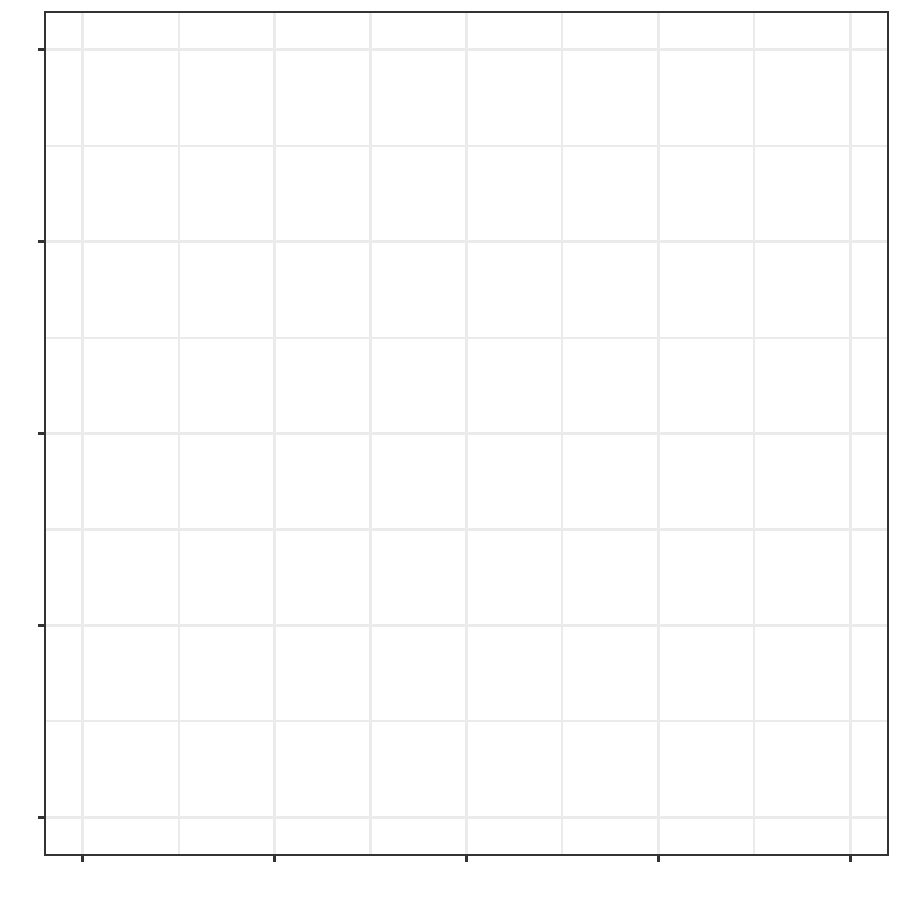
\includegraphics[width=\maxwidth]{img/desc-01-1} 

}


 
\clearpage
% -----------------------------------------------------------------------

\section{Aufgabe \hfill (7 Punkte)}

\textit{Geben Sie grunds{\"a}tzlich Formeln und Rechenweg zur L{\"o}sung der
  Teilaufgaben mit an!} \\[1Ex]

%% --------------------------------------------------------------------
\hfill\href{https://youtu.be/t0WYa_LVc5o}{
\includegraphics[width = 2cm]{img/youtube}}\\[1Ex]
%% --------------------------------------------------------------------



In einem Feldexperiment mit drei Bew{"a}sserungstypen ($low$, $mid$ und $high$) als Behandlung
(\textit{treatment}) ergeben sich die folgenden Barplots mit dem
gemessenen Frischgewicht (\textit{freshmatter}) von Kartoffeln.




{\centering 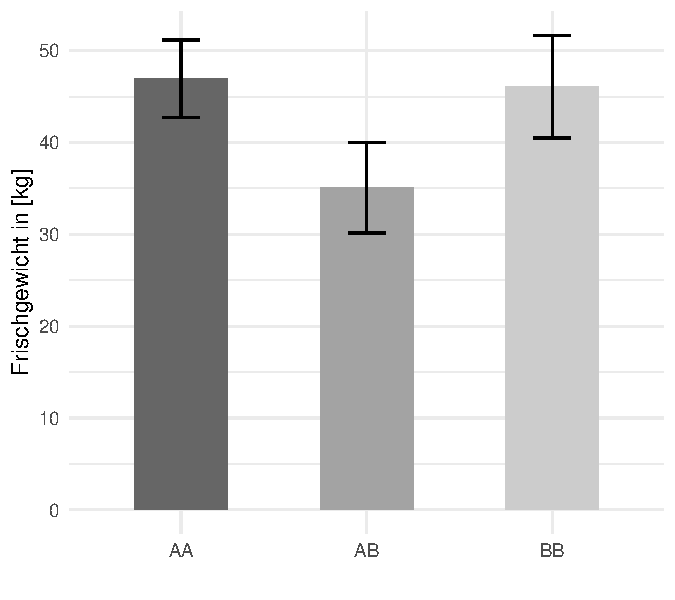
\includegraphics[width=\maxwidth]{img/barplot-02-1} 

}




\begin{enumerate}
\item Erstellen Sie eine Tabelle mit den statistischen Ma{\ss}zahlen aus der
  obigen Abbildung der drei Barplots! \textit{Beachten Sie die korrekte
    Darstellungsform der statistischen Ma{\ss}zahlen!} \textbf{(3 Punkte)}
\item Erstellen Sie einen beispielhaften Datensatz, aus dem die drei
  Barplots \textit{m{\"o}glicherweise} erstellt wurden, im \Rlogo {\"u}blichen Format! \textbf{(2 Punkte)}
\item Erwarten Sie einen Unterschied zwischen den Behandlungen? Begr{\"u}nden
  Sie Ihre Antwort! \textbf{(2 Punkte)}
\end{enumerate} 
\clearpage
% -----------------------------------------------------------------------

\section{Aufgabe \hfill (7 Punkte)}

\textit{Geben Sie grunds{\"a}tzlich Formeln und Rechenweg zur L{\"o}sung der
  Teilaufgaben mit an!} \\[1Ex]

%% --------------------------------------------------------------------
\hfill\href{https://youtu.be/vXnLttRL_VI}{
\includegraphics[width =
  2cm]{img/youtube}}\\[1Ex]
%% --------------------------------------------------------------------



In einem Freilandversuch mit drei Lichtstufen ($none$, $200lm$ und $600lm$) als Behandlung
(\textit{treatment}) ergibt sich die folgende Datentabelle mit dem
gemessenen Frischgewicht (\textit{freshmatter}) von Kartoffeln.

\begin{table}[!h]
\centering
\begin{tabular}{cc}
\toprule
treatment & freshmatter\\
\midrule
none & 48.4\\
600lm & 33.0\\
600lm & 20.5\\
200lm & 28.0\\
200lm & 29.8\\
\addlinespace
none & 28.8\\
none & 49.0\\
200lm & 26.3\\
none & 48.6\\
600lm & 36.6\\
\bottomrule
\end{tabular}
\end{table}



\begin{enumerate}
\item Zeichnen Sie in \textit{einer} Abbildung die Barplots f{\"u}r die
  Behandlung von Kartoffeln! Beschriften Sie die Achsen entsprechend!
  \textbf{(4 Punkte)}
\item Beschriften Sie \textit{einen} Barplot mit den g{\"a}ngigen
  statistischen Ma{\ss}zahlen! \textbf{(2 Punkte)}
\item Wenn Sie \textit{keinen Effekt} zwischen den Behandlungen von
  Kartoffeln erwarten w{\"u}rden, wie sehen dann die Barplots aus?
  \textbf{(1 Punkt)}
\end{enumerate} 
\clearpage
% -----------------------------------------------------------------------

\section{Aufgabe \hfill (9 Punkte)}

\textit{Geben Sie grunds{\"a}tzlich Formeln und Rechenweg zur L{\"o}sung der
  Teilaufgaben mit an!} \\[1Ex]

%% --------------------------------------------------------------------
\hfill\href{https://youtu.be/Xf0yE-o7bEU}{
\includegraphics[width = 2cm]{img/youtube}}\\[1Ex] %%youtube
%% --------------------------------------------------------------------



Nach einem Versuch in einer Klimakammer mit drei Substrattypen ($torf$, $40p60n$ und $70p30n$) als Behandlung
(\textit{treatment}) ergeben sich die folgenden Boxplots mit dem
gemessenen Trockengewicht (\textit{drymatter}) von Brokoli.



{\centering 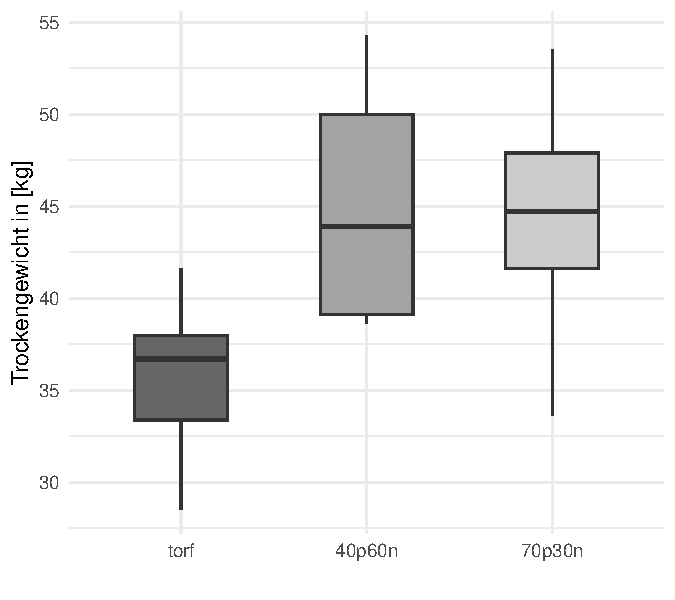
\includegraphics[width=\maxwidth]{img/boxplot-02-zer-1} 

}




\begin{enumerate}
\item Erstellen Sie eine Tabelle mit den statistischen Ma{\ss}zahlen aus der
  obigen Abbildung der drei Boxplots! \textit{Beachten Sie die korrekte
    Darstellungsform der statistischen Ma{\ss}zahlen!} \textbf{(3 Punkte)}
\item Beschriften Sie \textit{einen} der Boxplots mit den g{\"a}ngigen
  statistischen Ma{\ss}zahlen! \textbf{(2 Punkte)}
\item Erstellen Sie einen beispielhaften Datensatz, aus dem die drei
  Boxplots \textit{m{\"o}glicherweise} erstellt wurden, im \Rlogo {\"u}blichen Format! \textbf{(2 Punkte)}
\item Erwarten Sie einen Unterschied zwischen den Behandlungen? Begr{\"u}nden
  Sie Ihre Antwort! \textbf{(2 Punkte)}
\end{enumerate} 
\clearpage
% -----------------------------------------------------------------------

\section{Aufgabe \hfill (9 Punkte)}

\textit{Geben Sie grunds{\"a}tzlich Formeln und Rechenweg zur L{\"o}sung der
  Teilaufgaben mit an!} \\[1Ex]

%% --------------------------------------------------------------------
\hfill\href{https://youtu.be/0xc0jIPeiyw}{
\includegraphics[width =
  2cm]{img/youtube}}\\[1Ex]
%% --------------------------------------------------------------------



Nach einem Feldexperiment mit zwei Bew{"a}sserungstypen ($low$ und $high$) als Behandlung
(\textit{treatment}) ergibt sich die folgende Datentabelle mit dem
gemessenen Trockengewicht (\textit{drymatter}) von Maiss.

\begin{table}[!h]
\centering
\begin{tabular}{cc}
\toprule
treatment & drymatter\\
\midrule
low & 40.6\\
high & 32.5\\
low & 39.3\\
low & 39.1\\
low & 36.3\\
\addlinespace
high & 32.8\\
low & 31.6\\
high & 32.4\\
low & 44.8\\
high & 18.1\\
\addlinespace
low & 33.2\\
high & 34.5\\
high & 25.2\\
low & 30.6\\
high & 30.2\\
\addlinespace
low & 24.9\\
low & 36.5\\
high & 34.1\\
high & 26.6\\
low & 31.1\\
\addlinespace
high & 37.8\\
high & 24.0\\
\bottomrule
\end{tabular}
\end{table}



\begin{enumerate}
\item Zeichnen Sie in \textit{einer} Abbildung die beiden Boxplots f{\"u}r die
  zwei Behandlungen von Maiss! Beschriften Sie die Achsen entsprechend!
  \textbf{(6 Punkte)}
\item Beschriften Sie \textit{einen} der beiden Boxplots mit den g{\"a}ngigen
  statistischen Ma{\ss}zahlen! \textbf{(2 Punkte)}
\item Wenn Sie \textit{keinen Effekt} zwischen den Behandlungen von
  Maiss erwarten w{\"u}rden, wie sehen dann die beiden Boxplots aus?
  \textbf{(1 Punkt)}
\end{enumerate} 
\clearpage
% -----------------------------------------------------------------------

\section{Aufgabe \hfill (8 Punkte)}

\textit{Geben Sie grunds{\"a}tzlich Formeln und Rechenweg zur L{\"o}sung der
  Teilaufgaben mit an!} \\[1Ex]

%% --------------------------------------------------------------------
\hfill\href{https://youtu.be/aXvxGC4YLqk}{
\includegraphics[width =
  2cm]{img/youtube}}\\[1Ex]
%% --------------------------------------------------------------------



Nach einem Gew{\"a}chshausexperiment z{\"a}hlen Sie folgende Anzahl an L{\"a}sionen auf den
Bl{\"a}ttern von Brokoli nach einer durchgestandenen Infektion der Pflanze. 

\begin{center}
$6, 6, 2, 0, 2, 4, 5, 3, 4, 6, 5, 3, 4, 4, 7, 4, 2, 2, 2, 4, 1, 2, 2, 2, 3, 4, 6, 4, 2, 2$
\end{center}

\begin{enumerate}
\item Zeichen Sie ein Histogramm um die Verteilung der Daten zu visualisieren! (\textbf{3 Punkte})
\item Beschriften Sie die Achsen der Abbildung! (\textbf{2 Punkte})
\item Erg{\"a}nzen Sie die absoluten und relativen H{\"a}ufigkeiten in der
  Abbildung! \textbf{(1 Punkt)}
\item Berechnen Sie aus den Daten die \textit{Wahrscheinlichkeit}
  mehr als 4 L{\"a}sionen zu beobachten! \textbf{(1
    Punkt)}
\item Berechnen Sie aus den Daten die \textit{Chance} mehr
  als 4 L{\"a}sionen zu beobachten! \textbf{(1 Punkt)}
\end{enumerate}

 
\clearpage
% -----------------------------------------------------------------------

\section{Aufgabe \hfill (8 Punkte)}

\textit{Geben Sie grunds{\"a}tzlich Formeln und Rechenweg zur L{\"o}sung der
  Teilaufgaben mit an!} \\[1Ex]

%% --------------------------------------------------------------------
\hfill\href{https://youtu.be/ORHSPTCdfeY}{
\includegraphics[width =
  2cm]{img/youtube}}\\[1Ex]
%% --------------------------------------------------------------------



Nach einem Freilandexperiment bestimmen Sie folgende Trockengewichte von
Erdbeeren nach einer durchgestandenen Infektion der Pflanzen. 

\begin{center}
$13.4, 13.5, 9.5, 6.2, 11.8, 13.8, 14.8, 5.5, 8.3, 8.7, 6.6, 11.7, 12, 13.3, 10.4, 8.1, 5.1, 9.9, 8.5, 13.3$
\end{center}

\begin{enumerate}
\item Zeichen Sie ein Histogramm um die Verteilung der Daten zu
  visualisieren! (\textbf{3 Punkte})
 \item Erl{\"a}utern Sie Ihr Vorgehen um ein Histogramm f{\"u}r kontinuierliche
  Daten zu zeichnen!  (\textbf{2 Punkte})
\item Beschriften Sie die Achsen der Abbildung! (\textbf{2 Punkte})
\item Erg{\"a}nzen Sie die relativen H{\"a}ufigkeiten in der Abbildung! \textbf{(1
    Punkt)}  
\end{enumerate}

 
\clearpage
% -----------------------------------------------------------------------

\section{Aufgabe \hfill (10 Punkte)}

\textit{Geben Sie grunds{\"a}tzlich Formeln und Rechenweg zur L{\"o}sung der
  Teilaufgaben mit an!} \\[1Ex]

%% --------------------------------------------------------------------
\hfill\href{https://youtu.be/VAqiUdV4WQ0}{
\includegraphics[width =
  2cm]{img/youtube}}\\[1Ex]
%% --------------------------------------------------------------------

In einem Feldexperiment f{\"u}r die Bodendurchl{\"a}ssigkeit wurde der Niederschlag
pro Parzelle sowie der durchschnittliche Ertrag gemessen. Es ergibt sich
folgende Datentabelle. 

\begin{table}[!h]
\centering
\begin{tabular}{cc}
\toprule
water & drymatter\\
\midrule
15 & 18\\
15 & 21\\
17 & 19\\
17 & 19\\
17 & 17\\
\addlinespace
18 & 15\\
14 & 21\\
\bottomrule
\end{tabular}
\end{table}



\begin{enumerate}
\item Erstellen Sie den Scatter-Plot f{\"u}r die Datentabelle. Beschriften Sie
  die Achsen entsprechend! \textbf{(4 Punkte)}
\item Zeichnen Sie eine Gerade durch die Punkte! \textbf{(1 Punkt)}
\item Beschriften Sie die Gerade mit den g{\"a}ngigen statistischen Ma{\ss}zahlen!
  Geben Sie die numerischen Zahlenwerte mit an! \textbf{(3 Punkte)}
\item Wenn kein Effekt von dem Niederschlag auf das Trockengewicht
  vorhanden w{\"a}re, wie w{\"u}rde die Gerade verlaufen und welche Werte w{\"u}rden die
  statistischen Ma{\ss}zahlen annehmen? \textbf{(2 Punkt)}
\end{enumerate} 
\clearpage
% -----------------------------------------------------------------------

\section{Aufgabe \hfill (8 Punkte)}

\textit{Geben Sie grunds{\"a}tzlich Formeln und Rechenweg zur L{\"o}sung der
  Teilaufgaben mit an!} \\[1Ex]

%% --------------------------------------------------------------------
\hfill\href{https://youtu.be/t_1KL77mfmg}{
\includegraphics[width =
  2cm]{img/youtube}}\\[1Ex]
%% --------------------------------------------------------------------

Nach einem Feldexperiment mit zwei Pestiziden (\textit{RoundUp} und
\textit{OutEx}) ergibt sich die folgende Datentabelle mit dem jeweiligen
beobachteten Infektionsstatus bei Spargel.

\begin{table}[!h]
\centering
\begin{tabular}{cc}
\toprule
pesticide & infected\\
\midrule
OutEx & no\\
OutEx & no\\
RoundUp & no\\
RoundUp & no\\
OutEx & no\\
\addlinespace
RoundUp & yes\\
OutEx & no\\
RoundUp & no\\
OutEx & yes\\
RoundUp & no\\
\addlinespace
OutEx & yes\\
RoundUp & no\\
OutEx & no\\
OutEx & no\\
OutEx & no\\
\addlinespace
RoundUp & no\\
OutEx & yes\\
RoundUp & yes\\
OutEx & yes\\
RoundUp & no\\
\addlinespace
RoundUp & yes\\
RoundUp & yes\\
\bottomrule
\end{tabular}
\end{table}



\begin{enumerate}
\item Stellen Sie in einer 2x2 Tafel den Zusammenhang zwischen dem
  Pestizid und dem Infektionsstatus dar! \textbf{(4 Punkte)}
\item Zeichnen Sie den zugeh{\"o}rigen Mosaic-Plot. Berechnen Sie das
  Verh{\"a}ltnis pro Spalte! \textbf{(2 Punkte)}
\item Wenn das Pestizid keine Auswirkung auf den Infektionsstatus h{\"a}tte, wie
  sehe dann der Mosaic-Plot aus? \textbf{(2 Punkte)}
\end{enumerate} 
\clearpage
% -----------------------------------------------------------------------

\section{Aufgabe \hfill (10 Punkte)}

\textit{Geben Sie grunds{\"a}tzlich Formeln und Rechenweg zur L{\"o}sung der
  Teilaufgaben mit an!} \\[1Ex]

%% --------------------------------------------------------------------
\hfill\href{https://youtu.be/Op-gjzASH9I}{
\includegraphics[width =
  2cm]{img/youtube}}\\[1Ex]
%% --------------------------------------------------------------------



\begin{enumerate}
\item Zeichnen Sie {\"u}ber die untenstehenden Boxplots die entsprechende
  zugeh{\"o}rige Verteilung! \textbf{(3 Punkte)} 
\item Zeichnen Sie unter die untenstehenden Boxplots die entsprechende
  zugeh{\"o}rige Beobachtungen als Stiche! \textbf{(3 Punkte)}
\item Wieviel Prozent der Beobachtungen fallen in das IQR? Erg{\"a}nzen Sie die
  Abbildung entsprechend um den Bereich! \textbf{(2 Punkte)}
\item Wieviel Prozent der Beobachtungen fallen in $\pm 1s$ unter
  der Annahme einer Normalverteilung?  \textit{Wenn m{\"o}glich}, erg{\"a}nzen Sie
  die Abbildung entsprechend um den Bereich! \textbf{(2 Punkte)}
\end{enumerate}




{\centering 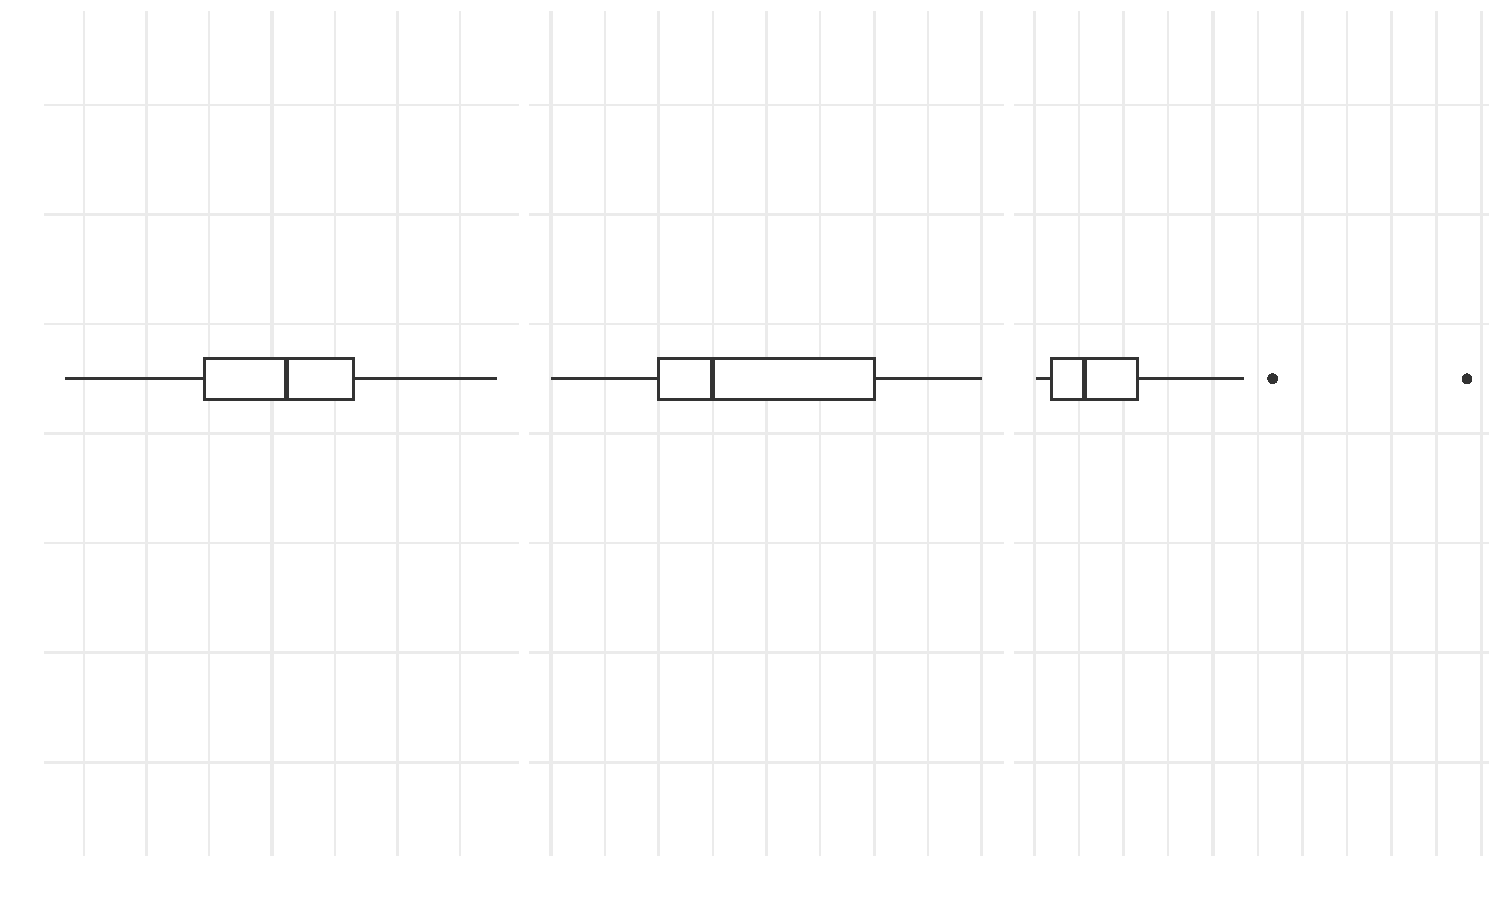
\includegraphics[width=\maxwidth]{img/desc-stat-11-1} 

}




 
\clearpage
% -----------------------------------------------------------------------

\section{Aufgabe \hfill (9 Punkte)}

\textit{Geben Sie grunds{\"a}tzlich Formeln und Rechenweg zur L{\"o}sung der
  Teilaufgaben mit an!} \\[1Ex]

%% --------------------------------------------------------------------
\hfill\href{https://youtu.be/ZrJhn2wPbq4}{
\includegraphics[width =
  2cm]{img/youtube}}\\[1Ex]
%% --------------------------------------------------------------------



\begin{enumerate}
\item Skizieren Sie $2$ Normalverteilungen \textit{in einer
    Abbildung} mit $\bar{y}_1 \neq \bar{y}_2$ und $s_1 \neq s_2$! \textbf{(3 Punkte)}
\item Beschriften Sie die Normalverteilungen mit den entsprechenden
  Parametern! \textbf{(2 Punkte)}
\item Erg{\"a}nzen Sie die Bereiche in der 68\% und 95\% der Beobachtungen
  fallen! Beschriften Sie die Grenzen der Bereiche mit der statistischen Ma{\ss}zahl! \textbf{(2 Punkte)}
\item Liegt Varianzhomogenit{\"a}t oder Varianzheterogenit{\"a}t vor? Begr{\"u}nden Sie
  Ihre Antwort! \textbf{(2 Punkte)}
\end{enumerate}

 
\clearpage
% -----------------------------------------------------------------------

\section{Aufgabe \hfill (9 Punkte)}

\textit{Geben Sie grunds{\"a}tzlich Formeln und Rechenweg zur L{\"o}sung der
  Teilaufgaben mit an!} \\[1Ex]

%% --------------------------------------------------------------------
\hfill\href{https://youtu.be/MiD42k4l5Ag}{
\includegraphics[width =
  2cm]{img/youtube}}\\[1Ex]
%% --------------------------------------------------------------------



\begin{enumerate}
\item Skizieren Sie in die unten stehenden, freien Abbildungen die
  Verteilungen, die sich nach der Abbildungs{\"u}berschrift ergeben! \textbf{(6
    Punkte)}
\item Beschriften Sie die Achsen der Abbildungen entsprechend! \textbf{(1
    Punkt)}
\item Achten Sie auf die entsprechende Skalierung der beiden Verteilungen
  in den Abbildungen! \textbf{(2 Punkte)}
\end{enumerate}



{\centering 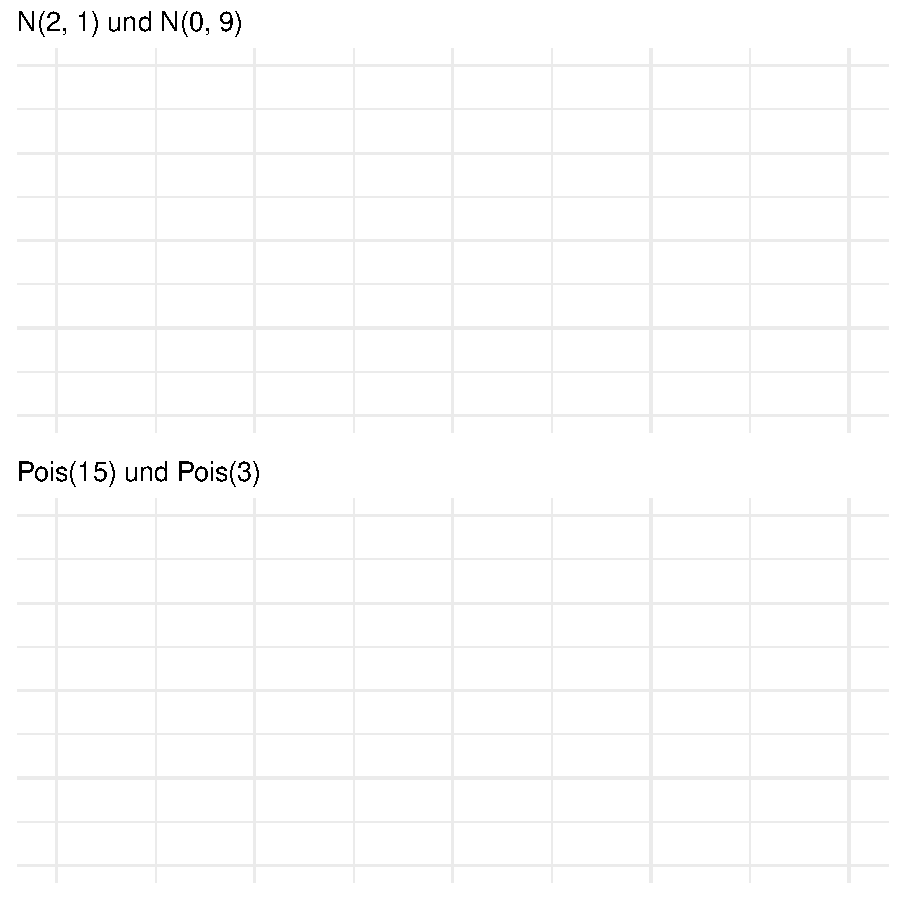
\includegraphics[width=\maxwidth]{img/histogram-01-1} 

}



 
\clearpage
% -----------------------------------------------------------------------
\begin{graybox}{Statistisches Testen}
Mehr Informationen zu den Aufgaben in den folgenden Kapiteln aus dem Skript Bio Data Science.
  \begin{itemize}
  \item \href{https://jkruppa.github.io/stat-tests-basic.html}{Kapitel 19 - Die Testentscheidung}
  \item \href{https://jkruppa.github.io/stat-tests-theorie.html}{Kapitel 20 - Die Testtheorie}
  \end{itemize}
\end{graybox}
\clearpage
% -----------------------------------------------------------------------  

\section{Aufgabe \hfill (9 Punkte)}

%% --------------------------------------------------------------------
\hfill\href{https://youtu.be/aHVYuFKTqZs}{
\includegraphics[width =
  2cm]{img/youtube}}\\[1Ex]
%% --------------------------------------------------------------------

Grundlage des statistischen Testen ist das Verst{\"a}ndnis von der
Grundgesamtheit (eng. \textit{population} oder \textit{ground truth}) und
der experimentellen Stichprobe (eng. \textit{sample}). 

\begin{enumerate}
\item Nennen Sie das statistische Verfahren und zwei konkrete Beispiele zur
  Durchf{\"u}hrung um von einer Grundgesamtheit auf eine Stichprobe zu
  gelangen! \textbf{(3 Punkte)}
\item Erkl{\"a}ren Sie den Zusammenhang zwischen Stichprobe und Grundgesamtheit
  an einem Schaubild! Beschriften Sie das Schaubild entsprechend!
  \textit{Nutzen Sie hierf{\"u}r als Veranschaulichung die K{\"o}rpergr{\"o}{\ss}e von
    M{\"a}nnern oder Frauen aus den Gummib{\"a}rchendaten!}  \textbf{(3 Punkte)}
\item Erweitern Sie das Schaubild um die Entstehung von $Pr(D|H_0)$!
  \textit{Nutzen Sie hierf{\"u}r als Veranschaulichung zus{\"a}tzlich die
    Gruppierungsvariable "`Modul"' aus den Gummib{\"a}rchendaten!}  \textbf{(3
    Punkte)}
\end{enumerate} 
\clearpage
% -----------------------------------------------------------------------

\section{Aufgabe \hfill (9 Punkte)}

%% --------------------------------------------------------------------
\hfill\href{https://youtu.be/Ric8ne39DtI}{
\includegraphics[width =
  2cm]{img/youtube}}\\[1Ex]
%% --------------------------------------------------------------------




F{\"u}r ein besseres Verst{\"a}ndnis der statistischen Testtheorie, auch
Null-Ritual genannt, kann eine Visualisierung als Kreuztabelle genutzt werden.  

\begin{enumerate}
\item Tragen Sie folgende statistische Fachbegriffe zur statistischen
  Testtheorie korrekt eine selbst erstellte Kreuztabelle ein! \textbf{(3
    Punkte)}
  \begin{center}
  \begin{tabular}{cccc}
  Testentscheidung & $\alpha$-Fehler & H$_0$ abgelehnt & H$_0$ beibehalten \\
  \end{tabular}
  \end{center}
\item Erg{\"a}nzen Sie Ihre erstellte Kreuztabelle um vier weitere, passende
  Fachbegriffe zur statistischen Testtheorie! \textbf{(2 Punkte)}
\end{enumerate}

Die Entscheidungsfindung durch einen statistischen Test kann auch durch die
Analogie zu einem Feuermelder abgebildet werden. Dabei symbolisiert der
Feuermelder den statistischen Test und es soll getestet werden, ob ein Feuer
ausgebrochen ist.

\begin{enumerate}
  \setcounter{enumi}{2}    
\item In der Analogie des Feuermelders, wie lautet der $\alpha$-Fehler? \textbf{(1 Punkt)}
\item In der Analogie des Feuermelders, wie lautet der $\beta$-Fehler? \textbf{(1 Punkt)}
\item Wenn der Feuermelder einmal pro Tag messen w{\"u}rde, wie oft w{\"u}rde der
  Feuermelder mit einem $\alpha$ von 5\% in einem halben Jahr Alarm schlagen?
  Begr{\"u}nden Sie Ihre Antwort! \textbf{(2 Punkte)}
\end{enumerate}



 
\clearpage
% -----------------------------------------------------------------------

\section{Aufgabe \hfill (9 Punkte)}

\textit{Geben Sie grunds{\"a}tzlich Formeln und Rechenweg zur L{\"o}sung der
  Teilaufgaben mit an!} \\[1Ex]

%% --------------------------------------------------------------------
\hfill\href{https://youtu.be/32JjH1eyuTU}{
\includegraphics[width =
  2cm]{img/youtube}}\\[1Ex]
%% --------------------------------------------------------------------



Abgebildet ist die t-Verteilung unter der Anahme der G{\"u}ltigkeit der
Nullhypothese. \textit{Beachten Sie, dass im Folgenden keine
  numerisch korrekte Darstellung verlangt wird! Es gilt Erkennbarkeit vor
  Genauigkeit!}

\begin{enumerate}
\item Erg{\"a}nzen Sie eine beschriftete $x$-Achse! \textbf{(1 Punkt)}
\item Erg{\"a}nzen Sie "`$\bar{y}_1 = \bar{y}_2$"'! \textbf{(1 Punkt)} 
\item Erg{\"a}nzen Sie "`$95\%$"'! \textbf{(1 Punkt)}
\item Zeichnen Sie $T_{\alpha=5\%}$ in die Abbildung! \textbf{(1 Punkt)} 
\item Zeichnen Sie das Signifikanzniveau $\alpha$ in die Abbildung! Begr{\"u}nden
  Sie Ihre Antwort! \textbf{(2 Punkte)} 
\item Zeichnen Sie $-T_{calc}$ in die Abbildung! \textbf{(1
    Punkt)}
\item Zeichnen Sie einen signifikant p-Wert in die Abbildung! Begr{\"u}nden
  Sie Ihre Antwort! \textbf{(2 Punkte)}   
\end{enumerate}



{\centering 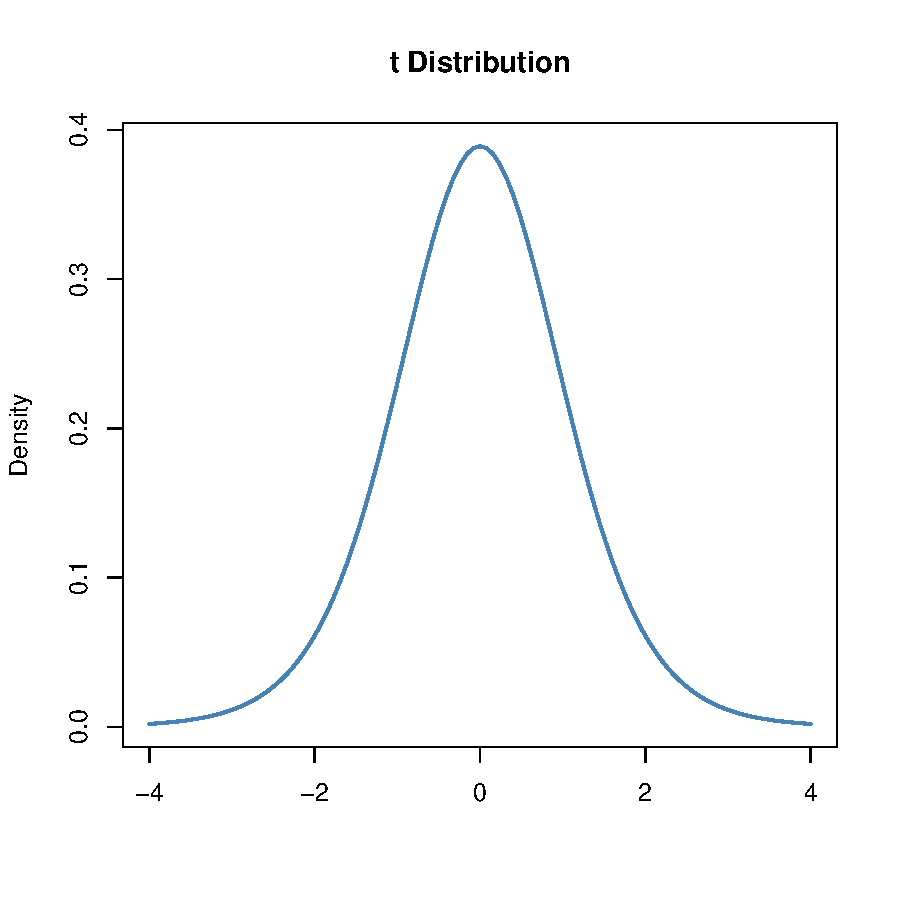
\includegraphics[width=\maxwidth]{img/statistisches-testen-3-1} 

}


 
\clearpage
% -----------------------------------------------------------------------

\section{Aufgabe \hfill (10 Punkte)}

%% --------------------------------------------------------------------
\hfill\href{https://youtu.be/CN_O4fYPbhs}{
\includegraphics[width =
  2cm]{img/youtube}}\\[1Ex]
%% --------------------------------------------------------------------



Sie rechnen einen t-Test f{\"u}r Gruppenvergleiche der Mittelwerte. Sie
sch{\"a}tzen den Unterschied zwischen dem mittleren Trockengewicht nach D{"u}ngergabe zu einer unbehandelten
Kontrolle.

\begin{enumerate}
\item Beschriften Sie die untenstehende Abbildung mit der
  Signifikanzschwelle! Begr{\"u}nden Sie Ihre Antwort! \textbf{(2 Punkte)}
\item Erg{\"a}nzen Sie eine \textit{in den Kontext passende} Relevanzschwelle!
  Begr{\"u}nden Sie Ihre Antwort! \textbf{(2 Punkte)} 
\item Skizieren Sie in die
  untenstehende Abbildung sechs einzelne Konfidenzintervalle (a-f) mit den
  jeweiligen Eigenschaften! \textbf{(6 Punkte)}
  \begin{itemize}
  \item[(a)] Ein signifikantes, nicht relevantes 95\% Konfidenzintervall 	
  \item[(b)] Ein 95\% Konfidenzintervall mit h{"o}herer Varianz $s_p$ in der Stichprobe als der Rest der 95\% Konfidenzintervalle 	
  \item[(c)] Ein nicht signifikantes, nicht relevantes 95\% Konfidenzintervall 	
  \item[(d)] Ein signifikantes, relevantes 90\% Konfidenzintervall. 
  \item[(e)] Ein 95\% Konfidenzintervall mit niedriger Varianz $s_p$ in der Stichprobe als der Rest 95\% der Konfidenzintervalle
  \item[(f)] Ein signifikantes, relevantes 95\% Konfidenzintervall
  \end{itemize}
\end{enumerate}

\begin{center}
  
\includegraphics[height = 12cm]{/Users/kruppajo/work/GitHub/exam/question/img/statistisches-testen-04}
\end{center}


 
\clearpage
% -----------------------------------------------------------------------

\section{Aufgabe \hfill (10 Punkte)}

\textit{Geben Sie grunds{\"a}tzlich Formeln und Rechenweg zur L{\"o}sung der
  Teilaufgaben mit an!} \\[1Ex]

%% --------------------------------------------------------------------
\hfill\href{https://youtu.be/FgZmpnEWDag}{
\includegraphics[width =
  2cm]{img/youtube}}\\[1Ex]
%% --------------------------------------------------------------------



Beim statistischen Testen gibt es einen Zusammenhang zwischen dem Effekt,
der Streuung sowie der Fallzahl. Gegeben sei die Formel f{\"u}r den Student
t-Test auf den die folgenden {\"U}berlegungen basieren sollen. Welche
Auswirkung hat die {\"A}nderungen der jeweiligen statistischen Ma{\ss}zahl des
Effekts $\Delta$, der Streuung $s$ und der Fallzahl $n$ auf die Teststistik
$T_{calc}$, den p-Wert $Pr(D|H_0)$ sowie dem Konfidenzintervall
$KI_{1-\alpha}$?

\begin{enumerate}
\item Visualisieren Sie den Zusammenhang zwischen der Teststatiatik
  $T_{calc}$ und dem p-Wert $Pr(D|H_0)$ f{\"u}r sich ver{\"a}ndernde $T_{calc}$-Werte!
  \textit{Geben Sie daf{\"u}r ein numerisches Beispiel in dem Sie drei
    $T_{calc}$-Werte und deren Einfluss auf den p-Wert vergleichen!}
  \textbf{(3 Punkte)}  
\item  F{\"u}llen Sie die untenstehende Tabelle aus in dem Sie die {\"A}nderung der
  statistischen Ma{\ss}zahlen auf die Teststatistik, den p-Wert sowie das
  Konfidenzintervall in \textit{einem} Wort oder Symbol beschreiben! \textbf{(4 Punkte)}
\begin{center}
  \large
  \begin{tabular}[c]{l|c|c|c|l|c|c|c}
    & $T_{calc}$ & $Pr(D|H_0)$ & $KI_{1-\alpha}$ & & $T_{calc}$ & $Pr(D|H_0)$ & $KI_{1-\alpha}$\strut\\ 
    \hline
    \textbf{$\Delta\; \uparrow$} & \hspace{1.8cm} & \hspace{1.8cm}  & \hspace{1.8cm} & \textbf{
                                                          $\Delta\; \downarrow$} &
                                                                          \hspace{1.8cm} & \hspace{1.8cm}  & \hspace{1.8cm}\strut\\
    \hline
        \textbf{$s\; \uparrow$} & \hspace{1.8cm} & \hspace{1.8cm}  & \hspace{1.8cm} & \textbf{
                                                          $s\; \downarrow$} &
                                                                          \hspace{1.8cm}
                                                & \hspace{1.8cm}  & \hspace{1.8cm}\strut\\
    \hline
        \textbf{$n\; \uparrow$} & \hspace{1.8cm} & \hspace{1.8cm}  & \hspace{1.8cm} & \textbf{
                                                          $n\; \downarrow$} &
                                                                          \hspace{1.8cm}
                                                & \hspace{1.8cm}  & \hspace{1.8cm}\strut\\
    \hline
  \end{tabular}
\end{center}
\item Visualisieren Sie ein 95\%-iges Konfidenzintervall im Vergleich
  zu einem 99\%-igen Konfidenzintervall! Begr{\"u}nden Sie Ihre Visualisierung anhand der Formel
  des Konfidenzintervalls des t-Tests mathematisch! \textbf{(3 Punkte)} 
\end{enumerate} 
\clearpage
% -----------------------------------------------------------------------
\begin{graybox}{Der t-Test}
Mehr Informationen zu den Aufgaben in den folgenden Kapiteln aus dem Skript Bio Data Science.
  \begin{itemize}
  \item \href{https://jkruppa.github.io/stat-tests-ttest.html}{Kapitel 22 - Der t-Test}
  \end{itemize}
\end{graybox}
\clearpage
% -----------------------------------------------------------------------

\section{Aufgabe \hfill (12 Punkte)}

\textit{Geben Sie grunds{\"a}tzlich Formeln und Rechenweg zur L{\"o}sung der
  Teilaufgaben mit an!} \\[1Ex]

%% --------------------------------------------------------------------
\hfill\href{https://youtu.be/Cq_rF_z4xOk}{
\includegraphics[width =
  2cm]{img/youtube}}\\[1Ex]
%% --------------------------------------------------------------------



Nach einem Experiment in einer Klimakammer mit zwei Pestiziden (\textit{RoundUp} und
\textit{GoneEx}) ergibt sich die folgende Datentabelle mit dem gemessenen
Trockengewicht (\textit{drymatter}) von Maiss.

\begin{table}[!h]
\centering
\begin{tabular}{cc}
\toprule
pesticide & drymatter\\
\midrule
GoneEx & 16\\
RoundUp & 17\\
RoundUp & 16\\
GoneEx & 18\\
RoundUp & 19\\
\addlinespace
GoneEx & 17\\
GoneEx & 16\\
GoneEx & 16\\
RoundUp & 22\\
GoneEx & 16\\
\addlinespace
RoundUp & 18\\
RoundUp & 22\\
\bottomrule
\end{tabular}
\end{table}



\begin{enumerate}
  \item Formulieren Sie die wissenschaftliche Fragestellung! \textbf{(1 Punkt)}
  \item Formulieren Sie das statistische Hypothesenpaar! \textbf{(2
      Punkte)}
  \item Bestimmen Sie die Teststatistik $T_{calc}$ eines Student t-Tests f{\"u}r den
  Vergleich der beiden Pestizide! \textbf{(5 Punkte)}
\item Treffen Sie mit $T_{\alpha = 5\%} = 2.68$ und dem berechneten $T_{calc}$ eine Aussage
  zur Nullhypothese! Begr{\"u}nden Sie Ihre Antwort! \textbf{(2 Punkte)}
\item Wenn Sie \textit{einen} Unterschied zwischen den beiden
  Pestiziden erwarten w{\"u}rden, wie gro{\ss} w{\"a}re dann die Teststatistik
  $T_{calc}$? Begr{\"u}nden Sie Ihre Antwort! \textbf{(2 Punkte)}
\end{enumerate} 
\clearpage
% -----------------------------------------------------------------------

\section{Aufgabe \hfill (8 Punkte)}

\textit{Geben Sie grunds{\"a}tzlich Formeln und Rechenweg zur L{\"o}sung der
  Teilaufgaben mit an!} \\[1Ex]

%% --------------------------------------------------------------------
\hfill\href{https://youtu.be/Cq_rF_z4xOk}{
\includegraphics[width =
  2cm]{img/caution}}\\[1Ex]
%% --------------------------------------------------------------------



Eine neue technische Anlage wurde in einem Experiment in einer Klimakammer getestet. Bei dem
Pilotexperiment mit sehr geringer Fallzahl $(n_g = 3)$ kamen zwei
Behandlungen (\textit{ctrl} und \textit{dose}) zum Einsatz. Es ergibt sich
die folgende Datentabelle mit dem gemessenen Gewicht (\textit{weight}) von
Erdbeeren.

\begin{table}[!h]
\centering
\begin{tabular}{cc}
\toprule
treatment & weight\\
\midrule
dose & 22.0\\
dose & 22.6\\
dose & 14.5\\
ctrl & 19.5\\
ctrl & 16.3\\
\addlinespace
ctrl & 18.9\\
\bottomrule
\end{tabular}
\end{table}



\begin{enumerate}
  \item Formulieren Sie das statistische Hypothesenpaar! \textbf{(2
      Punkte)}
  \item Bestimmen Sie die Teststatistik $T_{calc}$ eines Student t-Tests f{\"u}r den
  Vergleich der beiden Behandlungen! \textbf{(4 Punkte)}
\item Treffen Sie mit $T_{\alpha = 5\%} = 1.64$ und dem
  berechneten $T_{calc}$ eine Aussage zur Nullhypothese! Begr{\"u}nden Sie Ihre Antwort!  \textbf{(2 Punkte)}
\end{enumerate} 
\clearpage
% -----------------------------------------------------------------------

\section{Aufgabe \hfill (12 Punkte)}

\textit{Geben Sie grunds{\"a}tzlich Formeln und Rechenweg zur L{\"o}sung der
  Teilaufgaben mit an!} \\[1Ex]

%% --------------------------------------------------------------------
\hfill\href{https://youtu.be/TbSEOMCQYl4}{
\includegraphics[width =
  2cm]{img/youtube}}\\[1Ex]
%% --------------------------------------------------------------------



Nach einem Stallexperiment mit zwei Futtermitteln (\textit{FatDown} und
\textit{ProGain}) an H{"a}ngebauchschweinen ergibt sich die folgende Datentabelle
mit dem gemessenen Gewichtszunahmen nach f{\"u}nf Wochen Mast.

\begin{table}[!h]
\centering
\begin{tabular}{cc}
\toprule
feed & weight\\
\midrule
ProGain & 19\\
FatDown & 16\\
ProGain & 19\\
ProGain & 19\\
FatDown & 19\\
\addlinespace
ProGain & 18\\
FatDown & 17\\
FatDown & 16\\
ProGain & 17\\
ProGain & 19\\
\addlinespace
FatDown & 15\\
\bottomrule
\end{tabular}
\end{table}



\begin{enumerate}
  \item Formulieren Sie die wissenschaftliche Fragestellung! \textbf{(1 Punkt)}
  \item Formulieren Sie das statistische Hypothesenpaar! \textbf{(2
      Punkte)}
  \item Bestimmen Sie die Teststatistik $T_{calc}$ eines Welch t-Tests f{\"u}r den
  Vergleich der beiden Futtermittel! \textbf{(4 Punkte)}
\item Treffen Sie mit $T_{\alpha = 1\%} = 2.72$ und dem berechneten $T_{calc}$ eine Aussage
  zur Nullhypothese! Begr{\"u}nden Sie Ihre Antwort! \textbf{(2 Punkte)}
\item Berechnen Sie das 99\% Konfidenzintervall unter der
  Verwendung von $s_p$ und der gemittelten Fallzahl {\"u}ber die beiden Gruppen! \textbf{(2 Punkte)}
\item Nennen Sie den statistischen Grund, warum Sie sich zwischen einem Student t-Test und einem
  Welch t-Test entscheiden m{\"u}ssen! \textbf{(1 Punk)}
\end{enumerate} 
\clearpage
% -----------------------------------------------------------------------

\section{Aufgabe \hfill (11 Punkte)}

\textit{Geben Sie grunds{\"a}tzlich Formeln und Rechenweg zur L{\"o}sung der
  Teilaufgaben mit an!} \\[1Ex]

%% --------------------------------------------------------------------
\hfill\href{https://youtu.be/QR90zyn0Iz8}{
\includegraphics[width =
  2cm]{img/youtube}}\\[1Ex]
%% --------------------------------------------------------------------


Das Gewicht von K{\"u}ken wurde \textit{vor} der Behandlung mit STARTex und 1
Woche \textit{nach} der Behandlung gemessen. Es ergibt sich die folgende
Datentabelle.

\begin{table}[!h]
\centering
\begin{tabular}{ccc}
\toprule
animal\_id & before & after\\
\midrule
1 & 7 & 25\\
2 & 5 & 24\\
3 & 14 & 24\\
4 & 11 & 33\\
5 & 11 & 23\\
\addlinespace
6 & 11 & 26\\
7 & 7 & 28\\
\bottomrule
\end{tabular}
\end{table}



\begin{enumerate}
\item Formulieren Sie die Fragestellung! \textbf{(1 Punkt)}
\item Formulieren Sie das statistische Hypothesenpaar! \textbf{(2
    Punkte)}
\item Bestimmen Sie die Teststatistik $T_{calc}$ eines gepaarten t-Tests f{\"u}r den
  Vergleich der beiden Zeitpunkte! \textbf{(4 Punkte)}
\item Treffen Sie mit $T_{\alpha = 5\%} = 2.04$ und dem berechneten $T_{calc}$ eine Aussage
  zur Nullhypothese! Begr{\"u}nden Sie Ihre Antwort! \textbf{(2 Punkte)}
\item Sch{\"a}tzen Sie den $p$-Wert aus Ihrem berechneten $T_{calc}$ ab!
  Begr{\"u}nden Sie Ihre Antwort mit einer Skizze! \textbf{(2
    Punkte)}
\end{enumerate} 
\clearpage
% -----------------------------------------------------------------------

\section{Aufgabe \hfill (10 Punkte)}

%% --------------------------------------------------------------------
\hfill\href{https://youtu.be/exDo7AyHl4Q}{
\includegraphics[width =
  2cm]{img/youtube}}\\[1Ex]
%% --------------------------------------------------------------------

Sie erhalten folgende \Rlogo Ausgabe der Funktion \texttt{t.test()}.

\begin{knitrout}
\definecolor{shadecolor}{rgb}{0.969, 0.969, 0.969}\color{fgcolor}\begin{kframe}
\begin{verbatim}
## 
## 	Two Sample t-test
## 
## data:  drymatter by Fe
## t = 0.40711, df = 12, p-value = 0.6911
## alternative hypothesis: true  is not equal to [condensed]
## 95 percent confidence interval:
##  -3.771622  5.504955
## sample estimates:
## mean in group high mean in group trt2 
##           18.20000           17.33333
\end{verbatim}
\end{kframe}
\end{knitrout}


\begin{enumerate}
  \item Formulieren Sie die wissenschaftliche Fragestellung! \textbf{(2
Punkte)}
\item Liegt ein signifikanter Unterschied zwischen den Gruppen vor?
  Begr{\"u}nden Sie Ihre Antwort! \textbf{(2 Punkte)}
\item Skizieren Sie eine Abbildung in der Sie $T_{calc}$, $Pr(D|H_0)$, $A=0.95$,
  sowie $T_{\alpha=5\%} = |2.18|$ einzeichnen! \textbf{(4 Punkte)}
\item Beschriften Sie die Abbildung entsprechend! \textbf{(2 Punkte)}  
\end{enumerate} 
\clearpage
% -----------------------------------------------------------------------

\section{Aufgabe \hfill (8 Punkte)}

%% --------------------------------------------------------------------
\hfill\href{https://youtu.be/wJqsNV1hOW8}{
\includegraphics[width =
  2cm]{img/youtube}}\\[1Ex]
%% --------------------------------------------------------------------

Sie erhalten folgende \Rlogo Ausgabe der Funktion \texttt{t.test()}.

\begin{knitrout}
\definecolor{shadecolor}{rgb}{0.969, 0.969, 0.969}\color{fgcolor}\begin{kframe}
\begin{verbatim}
## 
## 	Two Sample t-test
## 
## data:  waterintake by infusion
## t = 1.118, df = 16, p-value = 0.2801
## alternative hypothesis: true  is not equal to [condensed]
## 95 percent confidence interval:
##  -1.493502  4.826835
## sample estimates:
## mean in group high  mean in group low 
##           16.33333           14.66667
\end{verbatim}
\end{kframe}
\end{knitrout}


\begin{enumerate}
  \item Formulieren Sie die wissenschaftliche Fragestellung! \textbf{(2
Punkte)}
\item Liegt ein signifikanter Unterschied zwischen den Gruppen vor?
  Begr{\"u}nden Sie Ihre Antwort! \textbf{(2 Punkte)}
\item Skizieren Sie das sich ergebende 95\% Konifidenzintervall! \textbf{(2 Punkte)}
\item Beschriften Sie die Abbildung und
  das 95\% Konfidenzintervall entsprechend! \textbf{(2 Punkte)}  
\end{enumerate} 
\clearpage
% -----------------------------------------------------------------------

\section{Aufgabe \hfill (9 Punkte)}

%% --------------------------------------------------------------------
\hfill\href{https://youtu.be/w62HJlbN28U}{
\includegraphics[width =
  2cm]{img/youtube}}\\[1Ex]
%% --------------------------------------------------------------------

Sie erhalten folgende \Rlogo Ausgabe der Funktion \texttt{t.test()}.

\begin{knitrout}
\definecolor{shadecolor}{rgb}{0.969, 0.969, 0.969}\color{fgcolor}\begin{kframe}
\begin{verbatim}
## 
## 	Welch t-Test
## 
## data:  drymatter by Fe
## t = 0.75701, df = 12, p-value = 0.4636
## alternative hypothesis: true  is not equal to [condensed]
## 95 percent confidence interval:
##  -1.961638  4.050526
## sample estimates:
## mean in group high mean in group trt1 
##           14.60000           13.55556
\end{verbatim}
\end{kframe}
\end{knitrout}


\begin{enumerate}
  \item Formulieren Sie die wissenschaftliche Fragestellung! \textbf{(2
Punkte)}
\item Liegt ein signifikanter Unterschied zwischen den Gruppen vor?
  Begr{\"u}nden Sie Ihre Antwort! \textbf{(2 Punkte)}
\item Skizieren Sie die sich ergebenden Boxplot!
  Welche Annahmen an die Daten haben Sie getroffen? Begr{\"u}nden Sie Ihre
  Antwort! \textbf{(3 Punkte)} 
\item Skizieren Sie die sich ergebenden Barplots! \textbf{(2 Punkte)} 
\end{enumerate}
 
\clearpage
% -----------------------------------------------------------------------

\section{Aufgabe \hfill (8 Punkte)}

%% --------------------------------------------------------------------
\hfill\href{https://youtu.be/kHmfEmU6lrk}{
\includegraphics[width =
  2cm]{img/youtube}}\\[1Ex]
%% --------------------------------------------------------------------


Sie erhalten folgende \Rlogo Ausgabe der Funktion \texttt{t.test()}.

\begin{knitrout}
\definecolor{shadecolor}{rgb}{0.969, 0.969, 0.969}\color{fgcolor}\begin{kframe}
\begin{verbatim}
## 
## 	Paired t-test
## 
## data:  drymatter by Fe
## t = -0.45496, df = 6, p-value = 0.6651
## alternative hypothesis: true  is not equal to [condensed]
## 95 percent confidence interval:
##  -8.200739  5.629310
## sample estimates:
## mean difference 
##       -1.285714
\end{verbatim}
\end{kframe}
\end{knitrout}


\begin{enumerate}
  \item Formulieren Sie das statistische Hypothesenpaar! \textbf{(2
Punkte)}
\item Liegt ein signifikanter Unterschied zwischen den Gruppen vor?
  Begr{\"u}nden Sie Ihre Antwort! \textbf{(2 Punkte)}
\item Skizzieren Sie den sich ergebenden Datensatz mit $n = 4$
  Beobachtungen! Die Daten m{\"u}ssen \textit{nicht} die Mittelwertsdifferenz
  $d$ erf{\"u}llen! \textbf{(2 Punkte)} 
\item Skizieren Sie den sich ergebenden Boxplot der Differenzen! Welche Annahmen an die Daten haben Sie getroffen? Begr{\"u}nden Sie Ihre Antwort! \textbf{(2 Punkte)} 
\end{enumerate}
 
\clearpage
% -----------------------------------------------------------------------
\begin{graybox}{Die ANOVA}
Mehr Informationen zu den Aufgaben in den folgenden Kapiteln aus dem Skript Bio Data Science.
  \begin{itemize}
  \item \href{https://jkruppa.github.io/stat-tests-anova.html}{Kapitel 23 - Die ANOVA}
  \end{itemize}
\end{graybox}
\clearpage
% -----------------------------------------------------------------------

\section{Aufgabe \hfill (8 Punkte)}

%% --------------------------------------------------------------------
\hfill\href{https://youtu.be/Q7xtQJoOmQI}{
\includegraphics[width =
  2cm]{img/youtube}}\\[1Ex]
%% --------------------------------------------------------------------



In einem Feldexperiment wurde der Ertrag von Maiss unter drei verschiedenen
Pestizid-Dosen $0.5 g/l$, $1.5 g/l$ und $2.5 g/l$ gemessen. Im Folgenden ist der
Datensatz einmal visualisiert.

\begin{knitrout}
\definecolor{shadecolor}{rgb}{0.969, 0.969, 0.969}\color{fgcolor}

{\centering 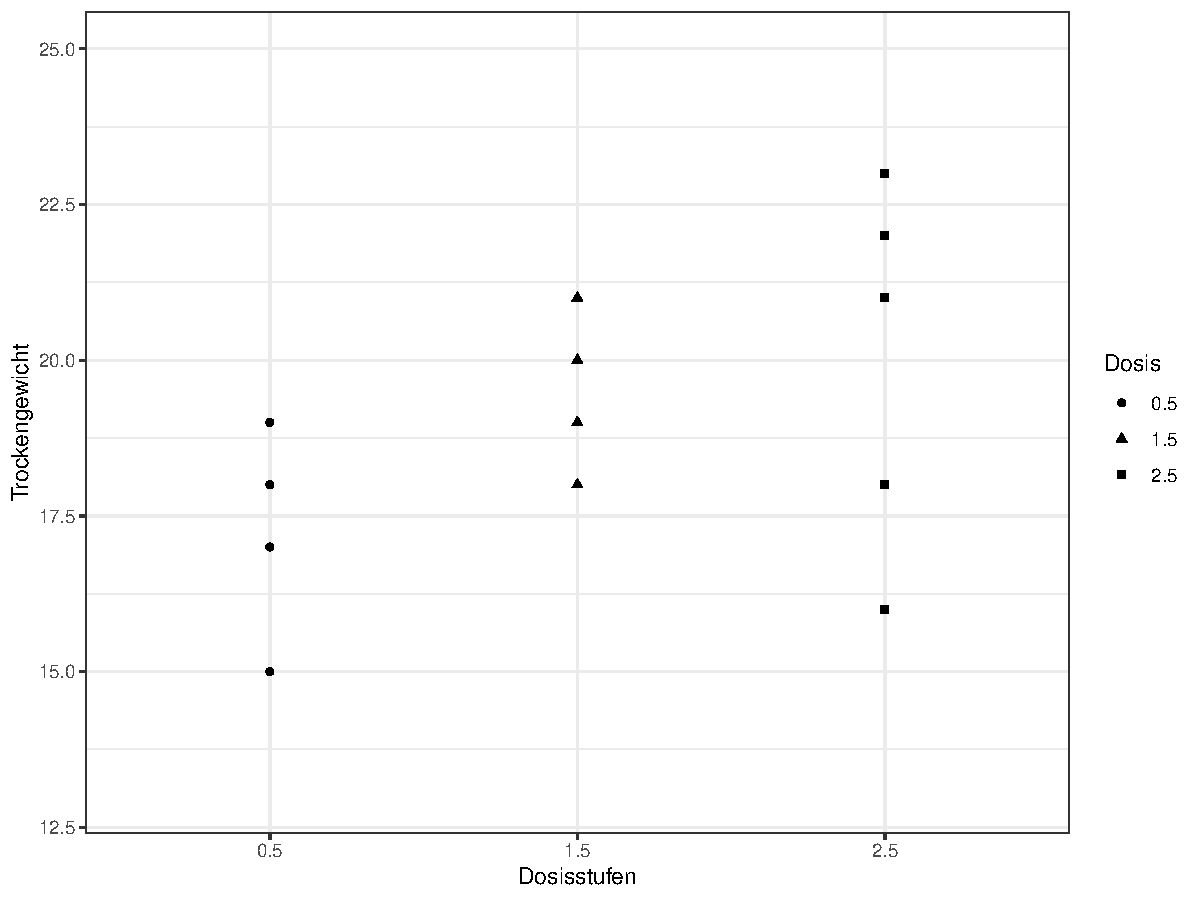
\includegraphics[width=\maxwidth]{img/anova-01-a-1} 

}


\end{knitrout}

\begin{enumerate}
\item Zeichnen Sie folgende statistischen Masszahlen in die Abildung ein!
  Beschriften Sie die statistischen Ma{\ss}zahlen! \textbf{(6 Punkte)}
  \begin{itemize}
  \item Globale Mittelwert: $\beta_0$
  \item Mittelwerte der einzelnen Dosen: $\bar{y}_{0.5}$, $\bar{y}_{1.5}$ und $\bar{y}_{2.5}$
  \item Effekt der einzelnen Dosen: $\beta_{0.5}$, $\beta_{1.5}$,
    und $\beta_{2.5}$
  \item Residuen oder Fehler: $\epsilon$
  \end{itemize}
\item Liegt ein \textit{vermutlicher} signifikanter Unterschied zwischen
  den Dosisstufen vor? Begr{\"u}nden Sie Ihre Antwort! \textbf{(2 Punkte)}
\end{enumerate}
 
\clearpage
% -----------------------------------------------------------------------

\section{Aufgabe \hfill (9 Punkte)}

\textit{Geben Sie grunds{\"a}tzlich Formeln und Rechenweg zur L{\"o}sung der
  Teilaufgaben mit an!} \\[1Ex]

%% --------------------------------------------------------------------
\hfill\href{https://youtu.be/49hvImMwVyE}{
\includegraphics[width =
  2cm]{img/caution}}\\[1Ex]
%% --------------------------------------------------------------------




Der Datensatz \texttt{week7\_growth\_tbl} enth{\"a}lt den Fettgehalt von
Mastschweinen, die unter einer Kontrolle und zwei verschiedenen
Behandlungsbedingungen erzielt wurden. Als Behandlung wurden verschiedene
Nahrungszus{\"a}tze in unterschiedlichen Dosen verf{\"u}ttert. Als Behandlung haben
Sie somit den Faktor \textit{group} mit den Faktorstufen
\textit{ctrl}, \textit{lethal} und
\textit{mid} vorliegen.



\begin{enumerate}
\item F{\"u}llen Sie die unterstehende einfaktorielle ANOVA Ergebnistabelle aus
  mit den gegebenen Informationen von \textbf{Df} und \textbf{Sum Sq}!
  \textbf{(3 Punkte)}
\end{enumerate}

\vspace{1Ex}

\begin{center}
  \Large
  \begin{tabular}{l|c|c|c|c|c}
     & \textbf{Df} & \textbf{Sum Sq} & \textbf{Mean Sq} & \textbf{F value} & \textbf{Pr(>F)} \strut\\
    \hline
   \textbf{group}  & 2 & 66.37 &  &  &  \strut\\
    \hline
   \textbf{error}  & 20 &  &  &  &  \strut\\
        \hline
   \textbf{total}  & 22 & 95.74 &  &  &  \strut\\
  \end{tabular}
\end{center}

\vspace{1Ex}

\begin{enumerate}
  \setcounter{enumi}{1}
\item Sch{\"a}tzen Sie den p-Wert der Tabelle mit der Information von
  $F_{\alpha = 5\%} = 3.49$ ab. Begr{\"u}nden Sie Ihre
  Antwort! \textbf{(2 Punkte)}
\item Berechen Sie den Effektsch{\"a}tzer $\eta^2$. Was sagt Ihnen der Wert von
  $\eta^2$ aus? \textbf{(2 Punkte)}
\item Skizzieren Sie K{\"o}rpergr{\"o}{\ss}e von f{"u}nf Tieren pro Behandlung f{\"u}r eine
  signifikante, einfaktorielle ANOVA! \textbf{(2 Punkte)}
\end{enumerate}



 
\clearpage
% -----------------------------------------------------------------------

\section{Aufgabe \hfill (12 Punkte)}

\textit{Geben Sie grunds{\"a}tzlich Formeln und Rechenweg zur L{\"o}sung der
  Teilaufgaben mit an!} \\[1Ex]

%% --------------------------------------------------------------------
\hfill\href{https://youtu.be/49hvImMwVyE}{
\includegraphics[width =
  2cm]{img/youtube}}\\[1Ex]
%% --------------------------------------------------------------------




Der Datensatz \texttt{fertilizer\_growth\_tbl} enth{\"a}lt den Ertrag pro Hektar der
Erbsenschoten, die unter einer Kontrolle und zwei
verschiedenen Behandlungsbedingungen erzielt wurden. Dabei wurden die
Erbsenschoten unter verschiedenen Konzentrationen von einem alternativen
D{\"u}nger angebaut. Als Behandlung haben Sie daher den Faktor \textit{group} mit den
Faktorstufen \textit{low}, \textit{extreme} und
\textit{mid} vorliegen.



\begin{enumerate}
\item F{\"u}llen Sie die unterstehende einfaktorielle ANOVA Ergebnistabelle aus
  mit den gegebenen Informationen von \textbf{Df} und \textbf{Sum Sq}!
  \textbf{(3 Punkte)}
\end{enumerate}

\vspace{1Ex}

\begin{center}
  \Large
  \begin{tabular}{l|c|c|c|c|c}
     & \textbf{Df} & \textbf{Sum Sq} & \textbf{Mean Sq} & \textbf{F value} & \textbf{Pr(>F)} \strut\\
    \hline
   \textbf{group}  & 2 & 23.52 &  &  &  \strut\\
    \hline
   \textbf{error}  & 18 & 26.29 &  &  &  \strut\\
  \end{tabular}
\end{center}

\vspace{1Ex}

\begin{enumerate}
  \setcounter{enumi}{1}
\item Sch{\"a}tzen Sie den p-Wert der Tabelle mit der Information von
  $F_{\alpha = 5\%} = 3.55$ ab. Begr{\"u}nden Sie Ihre
  Antwort! \textbf{(2 Punkte)}
\item Was bedeutet ein signifikantes Ergebnis in einer einfaktoriellen
  ANOVA im Bezug auf die m{\"o}glichen Unterschiede zwischen den Gruppen?
  Beziehen Sie sich auf den obigen Fragetext bei Ihrer Antwort!  \textbf{(2
    Punkte)}
\item Berechnen Sie \textit{einen} Student t-Test mit f{\"u}r den \textit{vermutlich}
  signifikantesten Gruppenvergleich anhand der untenstehenden Tabelle mit
  $T_{\alpha = 5\%} = 2.03$. Begr{\"u}nden Sie Ihre Auswahl! \textbf{(3 Punkte)}
\end{enumerate}

\begin{knitrout}
\definecolor{shadecolor}{rgb}{0.969, 0.969, 0.969}\color{fgcolor}\begin{table}[!h]
\centering
\begin{tabular}{cccc}
\toprule
group & n & mean & sd\\
\midrule
ctrl & 7 & 17.43 & 1.40\\
trt1 & 7 & 19.86 & 0.90\\
trt2 & 7 & 19.43 & 1.27\\
\bottomrule
\end{tabular}
\end{table}

\end{knitrout}

\begin{enumerate}
  \setcounter{enumi}{4}
\item Gegebenen der ANOVA Tabelle war das Ergebnis des t-Tests zu erwarten?
  Begr{\"u}nden Sie Ihre Antwort! \textbf{(2 Punkte)}
\end{enumerate}

 
\clearpage
% -----------------------------------------------------------------------

\section{Aufgabe \hfill (9 Punkte)}

%% --------------------------------------------------------------------
\hfill\href{https://youtu.be/d4CFR2MKX7I}{
\includegraphics[width =
  2cm]{img/youtube}}\\[1Ex]
%% --------------------------------------------------------------------




Der Datensatz \textit{crop\_tbl} enth{\"a}lt das Outcome \textit{height} f{\"u}r ein Feldexperiment mit 
Kartoffeln, welches unter drei 
verschiedenen D{\"u}ngerbedingungen erzielt wurden. Die D{\"u}ngerbedingungen sind in dem Faktor
\textit{trt} mit den Faktorstufen \textit{ctrl},  \textit{mid} und
 \textit{trt2} codiert. Sie erhalten folgenden Output in \Rlogo.

\begin{knitrout}
\definecolor{shadecolor}{rgb}{0.969, 0.969, 0.969}\color{fgcolor}\begin{kframe}
\begin{verbatim}
## Analysis of Variance Table
## 
## Response: height
##           Df Sum Sq Mean Sq F value  Pr(>F)
## trt        2 19.451  9.7253  4.5251 0.02392
## Residuals 20 42.984  2.1492
\end{verbatim}
\end{kframe}
\end{knitrout}

\begin{enumerate}
\item Stellen Sie die statistische $H_0$ und $H_A$ Hypothese f{\"u}r die obige
  einfaktorielle ANOVA auf! \textbf{(2 Punkte)}
\item Interpretieren Sie das Ergebnis der einfaktoriellen ANOVA! \textbf{(2 Punkt)} 
\item Berechen Sie den Effektsch{\"a}tzer $\eta^2$. Was sagt Ihnen der Wert von
  $\eta^2$ aus? \textbf{(2 Punkte)}
\item Skizieren Sie eine Abbildung, der dem obigen Ergebnis der
  einfaktoriellen ANOVA n{\"a}herungsweise entspricht! \textbf{(3 Punkte)}
\end{enumerate}

 
\clearpage
% -----------------------------------------------------------------------

\section{Aufgabe \hfill (12 Punkte)}

\textit{Geben Sie grunds{\"a}tzlich Formeln und Rechenweg zur L{\"o}sung der
  Teilaufgaben mit an!} \\[1Ex]

%% --------------------------------------------------------------------
\hfill\href{https://youtu.be/8Pb2sKUIMyk}{
\includegraphics[width =
  2cm]{img/youtube}}\\[1Ex]
%% --------------------------------------------------------------------



Der Datensatz \textit{tooth\_tbl} enth{\"a}lt Daten aus einer Studie zur
Bewertung der Wirkung von Vitamin C auf das Zahnwachstum bei
Meerschweinchen. Der Versuch wurde an verschiedenen Schweinen durchgef{\"u}hrt,
wobei jedes Tier eine von 4 Vitamin-C-Dosen \textit{dose}
{\"u}ber eine von 2 Verabreichungsmethoden \textit{supp}
erhielt. Die Zahnl{\"a}nge wurde als normalverteiltes Outcome gemessen.



\begin{enumerate}
\item F{\"u}llen Sie die unterstehende zweifaktorielle ANOVA Ergebnistabelle aus
  mit den gegebenen Informationen von \texttt{Df} und \texttt{Sum Sq}!
  \textbf{(4 Punkte)}
\item Sch{\"a}tzen Sie den p-Wert der Tabelle mit der Information von den
  $F_{\alpha = 5\%}$-Werten mit
  $F_{supp} = 4.26$ und
  $F_{dose} = 3.40$ sowie
  $F_{supp:dose} = 5.23$ ab. Begr{\"u}nden Sie Ihre
  Antwort! \textbf{(4 Punkte)}
\end{enumerate}

\vspace{1Ex}

\begin{center}
  \Large
  \begin{tabular}{l|c|c|c|c|c}
     & \textbf{Df} & \textbf{Sum Sq} & \textbf{Mean Sq} & \textbf{F value} & \textbf{Pr(>F)} \strut\\
    \hline
   \textbf{supp}  & 1 & 1.4 &  &  &  \strut\\
    \hline
    \textbf{dose}  & 3 & 119.4 &  &  &  \strut\\
    \hline
    \textbf{supp:dose}  & 3 & 59.55 &  &  &  \strut\\
    \hline
   \textbf{Residuals}  & 32 & 218.07 &  &  &  \strut\\
  \end{tabular}
\end{center}

\vspace{1Ex}

\begin{enumerate}
  \setcounter{enumi}{2}
\item Was bedeutet ein signifikantes Ergebnis in einer zweifaktoriellen
  ANOVA im Bezug auf die m{\"o}glichen Unterschiede zwischen den Gruppen?
  Beziehen Sie sich dabei einmal auf den Faktor \textit{supp} und einmal
  auf den Faktor \textit{dose}! \textbf{(2 Punkte)}
\item Was sagt der Term \textit{supp:dose} aus? Interpretieren Sie das
  Ergebnis des abgesch{\"a}tzten p-Wertes! \textbf{(2 Punkte)}
\end{enumerate}
 
\clearpage
% -----------------------------------------------------------------------

\section{Aufgabe \hfill (10 Punkte)}

%% --------------------------------------------------------------------
\hfill\href{https://youtu.be/rWTyHXXlYjY}{
\includegraphics[width =
  2cm]{img/youtube}}\\[1Ex]
%% --------------------------------------------------------------------



Der Datensatz \textit{pig\_gain\_weight\_tbl} enth{\"a}lt Daten aus einer Studie zur Bewertung
der Wirkung vom Vitamin Selen auf das Wachstum von Puten. Der
Versuch wurde an 63 Puten durchgef{\"u}hrt, wobei
jedes Tier eine von drei Selen-Dosen $dose$ ($0.1$ ng/Tag, $1$ ng/Tag und $20$ ng/Tag)
{\"u}ber eine von zwei Verabreichungsmethoden $form$ erhielt (Wasser oder
Festnahrung). Sie erhalten folgende Ausgabe in \Rlogo.

\begin{knitrout}
\definecolor{shadecolor}{rgb}{0.969, 0.969, 0.969}\color{fgcolor}\begin{kframe}
\begin{verbatim}
## Analysis of Variance Table
## 
## Response: weight
##           Df Sum Sq Mean Sq F value    Pr(>F)
## dose       2  13.77    6.89  0.5064    0.6110
## form       1 654.21  654.21 48.0996 1.759e-06
## dose:form  2 162.24   81.12  5.9643    0.0103
## Residuals 18 244.82   13.60
\end{verbatim}
\end{kframe}
\end{knitrout}

\begin{enumerate}
\item Stellen Sie die statistische $H_0$ und $H_A$ Hypothese f{\"u}r die obige
  zweifaktorielle ANOVA f{\"u}r den Faktor $dose$
  auf! \textbf{(2 Punkte)}
\item Interpretieren Sie das Ergebnis der zweifaktoriellen ANOVA. Gehen Sie
  im besonderen auf den Term $dose:form$ ein! \textbf{(2 Punkte)}
\item Zeichnen Sie eine Abbildung, der dem obigen Ergebnis der
  zweifaktoriellen ANOVA n{\"a}herungsweise entspricht! \textbf{(4 Punkte)}
\item Beschriften Sie die Abbildung entsprechend der \Rlogo Ausgabe! \textbf{(2 Punkte)}
\end{enumerate}
 
\clearpage
% -----------------------------------------------------------------------

\section{Aufgabe \hfill (8 Punkte)}


%% --------------------------------------------------------------------
\hfill\href{https://youtu.be/FjjJXkFJfIY}{
\includegraphics[width =
  2cm]{img/youtube}}\\[1Ex]
%% --------------------------------------------------------------------


In der untenstehenden Tabelle ist die Formel f{\"u}r den F-Test aus der ANOVA
und die Formel f{\"u}r den Student t-Test dargestellt. In der ANOVA berechnen
Sie die F-Statistik $F_{calc}$ und in dem Student t-Test die T-Statistik
$T_{calc}$.

\begin{center}
  \begin{tabular}{cc}
    $F_{calc} = \cfrac{MS_{treatment}}{MS_{error}}$ & $T_{calc} = \cfrac{\bar{y}_1 - \bar{y}_2}{s_p \cdot \sqrt{2/n_g}}$\\
  \end{tabular}
\end{center}


\begin{enumerate}
\item Erkl{\"a}ren Sie den konzeptionellen Zusammenhang zwischen der $F_{calc}$
  Statistik und $T_{calc}$ Statistik! \textbf{(2 Punkte)}
\item Visualisieren Sie eine nicht signifikante $F_{calc}$ Statistik sowie
  eine signifikante $F_{calc}$ Statistik anhand von $MS_{treatment}$ und
  $MS_{error}$! Beschriften Sie die Abbildung! \textbf{(2 Punkte)}
\item Erkl{\"a}ren Sie an der Formel des F-Tests sowie an der Abbildung warum
  das Minimum der F-Statistik 0 ist! \textbf{(2 Punkte)}
\item Wenn die F-Statistik 0 ist, spricht dies eher f{\"u}r oder gegen die
  Nullhypothese? Begr{\"u}nden Sie Ihre Antwort! \textbf{(2 Punkte)}
\end{enumerate}

 
\clearpage
% -----------------------------------------------------------------------

\section{Aufgabe \hfill (8 Punkte)}

%% --------------------------------------------------------------------
\hfill\href{https://youtu.be/2qG1Dws0MJo}{
\includegraphics[width =
  2cm]{img/youtube}}\\[1Ex]
%% --------------------------------------------------------------------


Sie rechnen eine zweifaktorielle ANOVA und erhalten einen signifikanten
Interaktionseffekt zwischen den beiden Faktoren $f_1$ und $f_2$. Der Faktor
$f_1$ hat drei Level. Der Faktor $f_2$ hat dagegen nur zwei Level.




\begin{enumerate}
\item Visualisieren Sie in zwei getrennten Abbildungen 
  eine schwache und eine starke Interaktion zwischen
  den Faktoren $f_1$ und $f_2$! \textbf{(4 Punkte)}
\item Erkl{\"a}ren Sie den Unterschied zwischen den beiden St{\"a}rken der Interaktion!
  \textbf{(2 Punkte)}
\item Wenn eine signifikante Interaktion in den Daten vorliegt, wie ist
  dann das weitere Vorgehen bei einem Posthoc-Test? 
  \textbf{(2 Punkte)}
\end{enumerate}

 
\clearpage
% -----------------------------------------------------------------------

\section{Aufgabe \hfill (9 Punkte)}

%% --------------------------------------------------------------------
\hfill\href{https://youtu.be/M9Uhm67ndxM}{
\includegraphics[width =
  2cm]{img/youtube}}\\[1Ex]
%% --------------------------------------------------------------------




Sie rechnen eine einfaktorielle ANOVA mit einem Faktor $f_1$ mit
drei Leveln. Nachdem Sie die einfaktorielle ANOVA gerechnet
haben, erhalten Sie einen p-Wert von $0.078$ und eine F Statistik mit
$F_{calc} = 1.2$. Als Sie sich die Boxplots der Behandlungen anschauen,
stellen Sie fest, dass es eigentlich einen Mittelwertsunterschied zwischen
dem ersten und zweiten Level geben m{\"u}sste. Die
$IQR$-Bereiche {\"u}berlappen sich nicht und die Mediane liegen auch weit vom
globalen Mittel entfernt.


\begin{enumerate}
\item Erkl{\"a}ren Sie die Annahme der Normalverteilung und die Annahme der
  Varianzhomogenit{\"a}t f{\"u}r eine ANOVA an einer passenden Abbildung! \textbf{(3 Punkte)}
\item Visualisieren Sie die Berechnung von $F_{calc}$ am obigen Beispiel!
  \textbf{(3 Punkte)}
\item Erkl{\"a}ren Sie das Ergebnis der obigen einfaktoriellen ANOVA unter der
  Ber{\"u}cksichtigung der Annahmen an eine ANOVA! \textbf{(3 Punkte)}
\end{enumerate}

 
\clearpage
% -----------------------------------------------------------------------
\begin{graybox}{Multiple Gruppenvergleiche}
Mehr Informationen zu den Aufgaben in den folgenden Kapiteln aus dem Skript Bio Data Science.
  \begin{itemize}
  \item \href{https://jkruppa.github.io/stat-tests-theorie.html}{Kapitel 20.3 Adjustierung für multiple Vergleiche}
  \item \href{https://jkruppa.github.io/stat-tests-posthoc.html}{Kapitel 31.7 Compact letter display}
  \end{itemize}
\end{graybox}
\clearpage
% ----------------------------------------------------------------------- 

\section{Aufgabe \hfill (8 Punkte)}

\textit{Geben Sie grunds{\"a}tzlich Formeln und Rechenweg zur L{\"o}sung der
  Teilaufgaben mit an!} \\[1Ex]

%% --------------------------------------------------------------------
 \hfill\href{https://youtu.be/hr_jPd1hpKY}{
\includegraphics[width =
   2cm]{img/youtube}}\\[1Ex]
%% --------------------------------------------------------------------


In einem Experiment zur Dosiswirkung wurden verschiedene Dosisstufen mit
einer Kontrollgruppe vergleichen. Es wurden verschiedene t-Test f{\"u}r den
Mittelwertsvergleich gerechnet und es ergab sich folgende Tabelle mit den
rohen p-Werten (\textit{Raw p-value}).


\begin{knitrout}
\definecolor{shadecolor}{rgb}{0.969, 0.969, 0.969}\color{fgcolor}\begin{table}[!h]
\centering\begingroup\fontsize{12}{14}\selectfont

\begin{tabular}{cccc}
\toprule
Vergleich & Raw p-value & Adjusted p-value & Reject Null\\
\midrule
dose 25 - ctrl & 0.030 &  & \\
dose 15 - ctrl & 0.020 &  & \\
dose 90 - ctrl & 0.070 &  & \\
dose 20 - ctrl & 0.012 &  & \\
\bottomrule
\end{tabular}
\endgroup{}
\end{table}

\end{knitrout}


%\begin{center}
%  \Large
%  \begin{tabular}{c|c|c|c}
%    \textbf{Vergleich} & \textbf{Raw p-val} & \textbf{Adjusted p-val} &
%                                                                        \textbf{Reject $\boldsymbol{H_0}$} \strut\\
%    \hline
%    dose 10 - ctrl  & pval_vec[1] &  &\strut\\
%    \hline
%    dose 15 - ctrl  & pval_vec[2] & &\strut\\
%    \hline
%    dose 20 - ctrl  & pval_vec[3] & &\strut\\
%    \hline
%    dose 40 - ctrl  & pval_vec[4] & &\strut\\
%  \end{tabular}
%\end{center}

\begin{enumerate}
\item F{\"u}llen Sie die Spalte "`Adjusted p-value"' mit den adjustierten
  p-Werten nach Bonferoni aus! \textbf{(4 Punkte)}
\item Entscheiden Sie, ob nach der Adjustierung die Nullhypothese weiter
  abgelehnt werden kann. Tragen Sie Ihre Entscheidung in die obige Tabelle
  ein. Begr{\"u}nden Sie Ihre Antwort! \textbf{(2 Punkte)}
\item Erkl{\"a}ren Sie warum die p-Werte bei multiplen Vergleichen
  adjustiert werden m{\"u}ssen! \textbf{(2 Punkte)}
\end{enumerate}

\vspace{1Ex}

 
\clearpage
% ----------------------------------------------------------------------- 

\section{Aufgabe \hfill (8 Punkte)}

\textit{Geben Sie grunds{\"a}tzlich Formeln und Rechenweg zur L{\"o}sung der
  Teilaufgaben mit an!} \\[1Ex]

%% --------------------------------------------------------------------
 \hfill\href{https://youtu.be/xq29O8qDrg0}{
\includegraphics[width =
   2cm]{img/youtube}}\\[1Ex]
%% --------------------------------------------------------------------


 
 In einem Experiment f{\"u}r den Zuckergehalt von Erdbeeren in g/kg mit f{\"u}nf
 Dosisstufen (ctrl, low, mid, high und pos) erhalten Sie folgendes \textit{Compact
   letter display (CLD)} als \Rlogo Ausgabe aus den rohen, unadjustierten
 $p$-Werten.



\begin{knitrout}
\definecolor{shadecolor}{rgb}{0.969, 0.969, 0.969}\color{fgcolor}\begin{kframe}
\begin{verbatim}
## ctrl high  low  mid  pos 
##  "a" "ab"  "c"  "b" "ab"
\end{verbatim}
\end{kframe}
\end{knitrout}

\begin{enumerate}
\item Zeichnen Sie eine Abbildung, der sich ergebenden Barplots! \textbf{(2 Punkte)}
\item Erg{\"a}nzen Sie das \textit{Compact letter display (CLD)} zu der
  Abbildung! \textbf{(1 Punkt)}
\item Erkl{\"a}ren Sie \textit{einen} Vorteil und \textit{einen} Nachteil des
  \textit{Compact letter display (CLD)}! \textbf{(2 Punkte)}
\item Erstellen Sie eine Matrix mit den paarweisen $p$-Werten, die sich
  n{\"a}herungsweise aus dem \textit{Compact letter display (CLD)} ergeben w{\"u}rde! Begr{\"u}nden Sie Ihre Antwort! \textbf{(3 Punkte)}
\end{enumerate}

 
\clearpage
% ----------------------------------------------------------------------- 

\section{Aufgabe \hfill (9 Punkte)}

\textit{Geben Sie grunds{\"a}tzlich Formeln und Rechenweg zur L{\"o}sung der
  Teilaufgaben mit an!} \\[1Ex]

%% --------------------------------------------------------------------
 \hfill\href{https://youtu.be/RagTFFKFbFg}{
\includegraphics[width =
   2cm]{img/youtube}}\\[1Ex]
%% --------------------------------------------------------------------



 
 In einem Experiment f{\"u}r den Zuckergehalt von Erdbeeren in g/kg mit vier
 Dosisstufen (ctrl, low, mid und high) erhalten Sie folgende Matrix als
 \Rlogo Ausgabe mit den rohen, unadjustierten $p$-Werten.



\begin{knitrout}
\definecolor{shadecolor}{rgb}{0.969, 0.969, 0.969}\color{fgcolor}\begin{kframe}
\begin{verbatim}
##           ctrl      high       low       mid
## ctrl 1.0000000 0.0187620 0.0202152 0.2416307
## high 0.0187620 1.0000000 0.0000251 0.2086938
## low  0.0202152 0.0000251 1.0000000 0.0009590
## mid  0.2416307 0.2086938 0.0009590 1.0000000
\end{verbatim}
\end{kframe}
\end{knitrout}

Im Weiteren erhalten Sie folgende Informationen {\"u}ber die Fallzahl $n$, den
Mittelwert $mean$ und die Standardabweichung $sd$ in den jeweiligen Dosisstufen.

\begin{knitrout}
\definecolor{shadecolor}{rgb}{0.969, 0.969, 0.969}\color{fgcolor}\begin{table}[!h]
\centering
\begin{tabular}{cccc}
\toprule
trt & n & mean & sd\\
\midrule
ctrl & 9 & 12.12 & 0.78\\
high & 9 & 8.38 & 4.31\\
low & 9 & 15.80 & 3.83\\
mid & 9 & 10.32 & 2.65\\
\bottomrule
\end{tabular}
\end{table}

\end{knitrout}


\begin{enumerate}
\item Zeichnen Sie in eine Abbildung, die sich ergebenden Barplots! \textbf{(2 Punkte)}
\item Adjustieren Sie die rohen $p$-Werte nach Bonferroni. Begr{\"u}nden Sie Ihre Antwort! \textbf{(3 Punkte)}
\item Erg{\"a}nzen Sie das \textit{Compact letter display (CLD)} zu der
  Abbildung. Nutzen Sie dazu die rohen $p$-Werte! \textbf{(2 Punkte)}
\item Interpretieren Sie das \textit{Compact letter display (CLD)}! \textbf{(2 Punkte)} 
\end{enumerate}

 
\clearpage
% -----------------------------------------------------------------------
  \begin{graybox}{Der $\mathcal{X}^2$-Test \& Der diagnostische Test}
Mehr Informationen zu den Aufgaben in den folgenden Kapiteln aus dem Skript Bio Data Science.
  \begin{itemize}
  \item \href{https://jkruppa.github.io/stat-tests-chi-test.html}{Kapitel 28 - Der $\mathcal{X}^2$-Test}
  \item \href{https://jkruppa.github.io/stat-tests-diagnostic.html}{Kapitel 29 - Der diagnostische Test}
  \end{itemize}
\end{graybox}
\clearpage
% -----------------------------------------------------------------------

\section{Aufgabe \hfill (11 Punkte)}

\textit{Geben Sie grunds{\"a}tzlich Formeln und Rechenweg zur L{\"o}sung der
  Teilaufgaben mit an!} \\[1Ex]

%% --------------------------------------------------------------------
\hfill\href{https://youtu.be/-Kva5wc5Elw}{\includegraphics[width =
  2cm]{img/youtube}}\\[1Ex]
%% --------------------------------------------------------------------




Nach einem Feldexperiment ergibt sich die folgende 2x2 Datentabelle mit einem
Pestizid (ja/nein) der Marke KillAll, dargestellt in den Zeilen, und
dem infizierten Pflanzenstatus (ja/nein) von Weizen, dargesellt in
den Spalten. Insgesamt wurden $n = 134$ Pflanzen untersucht.
\vspace{5Ex}

\begin{center}
  \Large
  \begin{tabular}{c|c|c|c}
     & \textbf{Erkrankt (ja)} & \textbf{Erkrankt (nein)} &  \strut\\
    \hline
    \textbf{Pestizid (ja)} & 38  & 21  &     \strut\\
    \hline
    \textbf{Pestizid (nein)} & 23  & 52  &      \strut\\
    \hline
     \phantom{100} & \phantom{100}  & \phantom{100}  &  \phantom{100}  \strut\\
  \end{tabular}
\end{center}

\vspace{5Ex}

\begin{enumerate}
\item Formulieren Sie die wissenschaftliche Fragestellung! \textbf{(1 Punkt)}
\item Erg{\"a}nzen Sie die Tabelle um die Randsummen! \textbf{(1 Punkt)} 
\item Berechnen Sie die Teststatistik eines Chi-Quadrat-Test auf der 2x2
  Tafel! \textbf{(3 Punkte)}
\item Treffen Sie eine Entscheidung im Bezug zu der Nullhypothese gegeben
  einem $\mathcal{X}^2_{\alpha = 5\%} = 3.841$! Begr{\"u}nden Sie Ihre Antwort!
  \textbf{(2 Punkte)}
\item Skizzieren Sie die $\mathcal{X}^2$-Verteilung, wenn die $H_0$ wahr
  ist! Erg{\"a}nzen Sie  $\mathcal{X}^2_{\alpha = 5\%}$ und
  $\mathcal{X}^2_{calc}$ in der Abbildung! \textbf{(2 Punkte)}
\item Berechnen Sie den Effektsch{\"a}tzer $Cramers\; V$! Interpretieren Sie den
  Effektsch{\"a}tzer! \textbf{(2 Punkte)}
\end{enumerate} 
\clearpage
% -----------------------------------------------------------------------

\section{Aufgabe \hfill (7 Punkte)}

\textit{Geben Sie grunds{\"a}tzlich Formeln und Rechenweg zur L{\"o}sung der
  Teilaufgaben mit an!} \\[1Ex]

%% --------------------------------------------------------------------
\hfill\href{https://youtu.be/jakM7fHyZfU}{\includegraphics[width =
  2cm]{img/youtube}}\\[1Ex]
%% --------------------------------------------------------------------




Gegeben sind folgende Randsummen in einer 2x2 Kreuztabelle aus einem
Experiment mit $n = 135$ Sauen. In dem Experiment wurde gemessen,
ob eine Sau nach einer Behandlung mit einem Medikament (ja/nein)
mehr als 30 Ferkel pro Jahr bekommen konnte (ja/nein).

\vspace{5Ex}

\begin{center}
  \Large
  \begin{tabular}{c|c|c|c}
     & \textbf{>30 Ferkel (ja)} & \textbf{$\leq$30 Ferkel (nein)} &  \strut\\
    \hline
    \textbf{Medikament (ja)} & \phantom{100}  & \phantom{100}  &   76  \strut\\
    \hline
    \textbf{Medikament (nein)} & \phantom{100}  & \phantom{100}  &   59   \strut\\
    \hline
     &  89 &  46 &  135  \strut\\
  \end{tabular}
\end{center}



\vspace{5Ex}

\begin{enumerate}
\item Erg{\"a}nzen Sie die Felder innerhalb der 2x2 Kreuztabelle in dem Sinne,
  dass \textit{ein} signifikanter Effekt zu erwarten w{\"a}re!
  \textbf{(2 Punkte)}
\item Erkl{\"a}ren und Begr{\"u}nden Sie Ihr Vorgehen an der Formel des
  Chi-Quadrat-Tests mit
  \begin{equation*}
  \mathcal{X}^2 = \sum\tfrac{(O - E)^2}{E}.  
  \end{equation*}
  Sie k{\"o}nnen dies an einem Beispiel erkl{\"a}ren! \textbf{(2 Punkte)}
\item Was ist die Mindestanzahl an Beobachtungen je Zelle? Wenn in einer
  der Zellen weniger Beobachtungen auftreten, welchen Test k{\"o}nnen Sie
  anstatt des "`normalen"' Chi-Quadrat-Tests anwenden? \textbf{(2 Punkte)}
\item Warum hat die obige Vierfeldertafel einen Freiheitsgrad von $df=1$?
  \textbf{(1 Punkt)}
\end{enumerate} 
\clearpage
% -----------------------------------------------------------------------

\section{Aufgabe \hfill (10 Punkte)}

%% --------------------------------------------------------------------
\hfill\href{https://youtu.be/ghArbetOr_E}{\includegraphics[width =
  2cm]{img/youtube}}\\[1Ex]
%% --------------------------------------------------------------------

Nach einem Experiment erhalten Sie folgende 2x2 Kreuztabelle aus Ihren
erhobenen Daten.

\begin{knitrout}
\definecolor{shadecolor}{rgb}{0.969, 0.969, 0.969}\color{fgcolor}\begin{kframe}
\begin{verbatim}
##                  Verschimmelt
## Gruppe            yes no
##   Papageien-Tulpe   6  3
##   Zwerg-Tulpe       6  4
\end{verbatim}
\end{kframe}
\end{knitrout}

Aus der 2x2 Kreuztabelle erhalten Sie folgende \Rlogo Ausgabe der Funktion
\texttt{fisher.test()}.

\begin{knitrout}
\definecolor{shadecolor}{rgb}{0.969, 0.969, 0.969}\color{fgcolor}\begin{kframe}
\begin{verbatim}
## 
## 	Fisher's Exact Test for Count Data
## 
## data:  mat
## p-value = 1
## alternative hypothesis: true odds ratio is not equal to 1
## 95 percent confidence interval:
##   0.1442262 13.2691123
## sample estimates:
## odds ratio 
##   1.313276
\end{verbatim}
\end{kframe}
\end{knitrout}


\begin{enumerate}
\item Formulieren Sie die wissenschaftliche Fragestellung! \textbf{(2 Punkte)}
\item Liegt ein signifikanter Unterschied zwischen den Gruppen vor?
  Begr{\"u}nden Sie Ihre Antwort! \textbf{(2 Punkte)}
\item Skizieren Sie das sich ergebende 95\% Konifidenzintervall! \textbf{(2 Punkte)}
\item Beschriften Sie die Abbildung und
  das 95\% Konfidenzintervall entsprechend! \textbf{(2 Punkte)} 
\item Interpretieren Sie das \textit{Odds ratio} im Kontext der
  wissenschaftlichen Fragestellung! \textbf{(2 Punkte)} 
\end{enumerate}
 
\clearpage
% -----------------------------------------------------------------------

\section{Aufgabe \hfill (11 Punkte)}

%% --------------------------------------------------------------------
\hfill\href{https://youtu.be/VQlNl8hvRII}{\includegraphics[width =
  2cm]{img/youtube}}\\[1Ex]
%% --------------------------------------------------------------------


Die Pr{\"a}valenz von Klauenseuche bei Wollschweinen wird mit
4\% angenommen. In 85\% der F{\"a}lle ist ein Test positiv, wenn das Wollschwein erkrankt
ist. In 8.5\% der F{\"a}lle ist ein Test positiv,
wenn das Wollschwein \textit{nicht} erkrankt ist und somit gesund ist. Sie
werten 1000 Wollschweine mit einem
diagnostischen Test auf Klauenseuche aus.



\begin{enumerate}
\item F{\"u}llen und beschriften Sie den untenstehenden Doppelbaum! Beschriften
  Sie auch die {\"A}ste des Doppelbaumes, mit denen Ihnen bekannten
  Informationen!  \textbf{(8 Punkte)}
\item Berechnen Sie die Wahrscheinlichkeit $Pr(K^+|T^+)$! \textbf{(2 Punkte)}
\item Was sagt Ihnen die Wahrscheinlichkeit $Pr(K^+|T^+)$ aus? \textbf{(1 Punkt)}
\end{enumerate}

\vspace{1cm}

\begin{center}
  \includegraphics[width=17cm]{/Users/kruppajo/work/GitHub/exam/question/img/diag-doppelbaum}
\end{center}



 
\clearpage
% -----------------------------------------------------------------------

\section{Aufgabe \hfill (12 Punkte)}


%% --------------------------------------------------------------------
\hfill\href{https://youtu.be/_7s44pbOc00}{\includegraphics[width =
  2cm]{img/youtube}}\\[1Ex]
%% --------------------------------------------------------------------





Folgender diagnostischer Doppelbaum nach der Testung auf Klauenseuche bei
Fleckvieh ist gegeben.

\begin{enumerate}
\item F{\"u}llen und beschriften Sie den untenstehenden Doppelbaum! \textbf{(4
    Punkte)}
\item Berechnen Sie die Wahrscheinlichkeit $Pr(K^+|T^+)$! \textbf{(2 Punkte)}
\item Berechnen Sie die Pr{\"a}valenz f{\"u}r Klauenseuche! \textbf{(2 Punkte)}
\item Berechnen Sie die Sensifit{\"a}t und Spezifit{\"a}t des diagnostischen Tests
  f{\"u}r Klauenseuche! Erstellen Sie daf{\"u}r zun{\"a}chst eine 2x2 Kreuztabelle aus
  dem ausgef{\"u}llten Doppelbaum!
  \textbf{(4 Punkte)}
\end{enumerate}

\vspace{1cm}
 
\begin{tikzpicture}
  \node (image) at (0,0) {
    \includegraphics[width=\textwidth]{/Users/kruppajo/work/GitHub/exam/question/img/diag-doppelbaum}
  };
  \node[] at (-4.8,0) {\huge 180};
  \node[] at (-1.7,0) {\huge 20};
  \node[] at (1.7,0) {\huge 850};
  \node[] at (4.75,0) {\huge 1800};
\end{tikzpicture}




 
\clearpage
% -----------------------------------------------------------------------

\section{Aufgabe \hfill (10 Punkte)}

%% --------------------------------------------------------------------
\hfill\href{https://youtu.be/G-_r2KplGTI}{\includegraphics[width =
  2cm]{img/youtube}}\\[1Ex]
%% --------------------------------------------------------------------


Beim diagnostischen Testen erhalten Sie \textit{True Positives (TP)},
\textit{True Negatives (TN)}, \textit{False Positives (FP)} und
\textit{False Negatives (FN)}. Erkl{\"a}ren Sie den Zusammenhang wir folgt.

\begin{enumerate}
\item Tragen Sie \textit{TP}, \textit{TN}, \textit{FP} und \textit{FN} in
  eine 2x2 Kreuztablle ein. Beschriften Sie die Tabelle entsprechend!
  \textbf{(2 Punkte)}
\item Visualisieren Sie \textit{TP}, \textit{TN}, \textit{FP} und
  \textit{FN} in einer Abbildung. Beschriften Sie die Abbildung und die
  Achsen entsprechend! \textbf{(4 Punkte)}
\item Erkl{\"a}ren Sie an einem numerischen Beispiel und der Abbildung die
  Berechnung der Pr{\"a}valenz!  \textbf{(2 Punkte)}
\item Erkl{\"a}ren Sie an einem Schaubild den Unterschied zwischen Inzidenz und
  Pr{\"a}valenz!  \textbf{(2 Punkte)}
\end{enumerate}





 
\clearpage
% -----------------------------------------------------------------------
\begin{graybox}{Nicht parametrische Tests}
Mehr Informationen zu den Aufgaben in den folgenden Kapiteln aus dem Skript Bio Data Science.
  \begin{itemize}
  \item \href{https://jkruppa.github.io/stat-tests-utest.html}{Kapitel 25 - Der Wilcoxon-Mann-Whitney-Test}
  \item \href{https://jkruppa.github.io/stat-tests-kruskal.html}{Kapitel 26 - Der Kruskal-Wallis-Test}
  \end{itemize}
\end{graybox}
\clearpage
% -----------------------------------------------------------------------

\section{Aufgabe \hfill (12 Punkte)}

\textit{Geben Sie grunds{\"a}tzlich Formeln und Rechenweg zur L{\"o}sung der
  Teilaufgaben mit an!} \\[1Ex]

%% --------------------------------------------------------------------
\hfill\href{https://youtu.be/ArHA6MZOEOw}{\includegraphics[width =
  2cm]{img/youtube}} %%youtube
\hspace{2Ex}
%% --------------------------------------------------------------------


Die Anzahl an Nematoden wurde vor und nach einer Behandlung mit einem
bioaktiven D{\"u}nger gez{\"a}hlt. Es ergibt sich folgende Datentabelle.

\begin{table}[!h]
\centering
\begin{tabular}{ccccccc}
\toprule
Vorher & Nachher & Differenz & Vorzeichen & Rang & Positiv Rang & Negativ Rang\\
\midrule
8 & 10 &  &  &  &  & \\
8 & 13 &  &  &  &  & \\
11 & 11 &  &  &  &  & \\
9 & 12 &  &  &  &  & \\
12 & 12 &  &  &  &  & \\
\addlinespace
7 & 10 &  &  &  &  & \\
10 & 10 &  &  &  &  & \\
11 & 11 &  &  &  &  & \\
13 & 11 &  &  &  &  & \\
10 & 13 &  &  &  &  & \\
\addlinespace
10 & 13 &  &  &  &  & \\
11 & 13 &  &  &  &  & \\
14 & 12 &  &  &  &  & \\
8 & 11 &  &  &  &  & \\
8 & 13 &  &  &  &  & \\
\bottomrule
\end{tabular}
\end{table}



\begin{enumerate}
\item Erg{\"a}nzen Sie die obige Tabelle mit den notwendigen Informationen, die
  Sie ben{\"o}tigen um einen Wilcoxon-Vorzeichen-Rang-Test zu rechnen!
  \textbf{(4 Punkte)}
\item Bestimmen Sie die Teststatistik $W$ mit $W = \min(T_{-}; T_{+})$ und
  berechnen Sie den erwarteten Wert $\mu_W = \cfrac{n_{!0} \cdot (n_{!0} + 1)}{4}$!
  \textbf{(2 Punkte)}
\item Berechnen Sie anschlie{\ss}end den $z$-Wert mit $z = \cfrac{W -
    \mu_W}{11.247}$! \textbf{(2 Punkte)}
\item Liegt mit einer Signifikanzschwelle von $z_{\alpha = 5\%} =
  1.96$ ein Unterschied zwischen den beiden Zeitpunkten vor? Begr{\"u}nden Sie
  Ihre Antwort! \textbf{(2 Punkte)} 
\item Berechnen Sie die Effektst{\"a}rke mit $r = |\frac{z}{\sqrt{n}}| $ und
  interpretieren Sie die Effektst{\"a}rke! \textbf{(2 Punkte)} 
\end{enumerate} 
\clearpage
% ----------------------------------------------------------------------- 

\section{Aufgabe \hfill (8 Punkte)}

\textit{Geben Sie grunds{\"a}tzlich Formeln und Rechenweg zur L{\"o}sung der
  Teilaufgaben mit an!} \\[1Ex]

%% --------------------------------------------------------------------
\hfill\href{https://youtu.be/5tiJFxuZcco}{\includegraphics[width =
  2cm]{img/youtube}} %%youtube
\hspace{2Ex}
%% --------------------------------------------------------------------




Nach einer Behandlung mit RootsGoneX wurde die mittelere Anzahl an Wurzeln
an der invasiven Lupine (\textit{Lupinus polyphyllus}) gez{\"a}hlt. Es ergab sich
folgender Datensatz an mittleren Wurzelanzahl.

\begin{knitrout}
\definecolor{shadecolor}{rgb}{0.969, 0.969, 0.969}\color{fgcolor}\begin{table}[!h]
\centering
\begin{tabular}{cc}
\toprule
Treatment & Count\\
\midrule
RootsGoneX & 11.1\\
Kontrolle & 2.4\\
Kontrolle & 3.9\\
Kontrolle & 7.1\\
Kontrolle & 5.1\\
\addlinespace
RootsGoneX & 11.8\\
Kontrolle & 1.6\\
Kontrolle & 5.1\\
RootsGoneX & 10.7\\
Kontrolle & 2.9\\
\addlinespace
RootsGoneX & 11.6\\
\bottomrule
\end{tabular}
\end{table}

\end{knitrout}

Rechnen Sie einen Mann-Whitney-U-Test auf den obigen Daten.

\begin{enumerate}
\item Bestimmen Sie hierf{\"u}r $U_c$ mit $U_c = n_1n_2 +
  \cfrac{n_1(n_1+1)}{2}-R_1$! \textbf{(4 Punkte)} 
\item Geben Sie eine Aussage {\"u}ber die Signifikanz von $U_c$ durch
  $z = \cfrac{U_c -
    \cfrac{n_1n_2}{2}}{\sqrt{\cfrac{n_1n_2(n_1+n_2+1)}{12}}}$ und dem
  kritischen Wert von $z_{\alpha = 5\%} = 1.96$. Begr{\"u}nden Sie Ihre
  Antwort! \textbf{(2 Punkte)}
\item Berechnen Sie die Effektst{\"a}rke mit $r = |\frac{z}{\sqrt{n}}| $ und
  interpretieren Sie die Effektst{\"a}rke! \textbf{(2 Punkte)} 
\end{enumerate} 
\clearpage
% -----------------------------------------------------------------------  

\section{Aufgabe \hfill (10 Punkte)}

\textit{Geben Sie grunds{\"a}tzlich Formeln und Rechenweg zur L{\"o}sung der
  Teilaufgaben mit an!} \\[1Ex]

%% --------------------------------------------------------------------
\hfill\href{https://youtu.be/gC0SXiIG2wQ}{\includegraphics[width =
  2cm]{img/youtube}} %%youtube
\hspace{2Ex}
%% --------------------------------------------------------------------




Die Anzahl an Bl{\"u}ten der Vanilleplanze pro Box wurde nach der Gabe von
zus{\"a}tzlichen Phosporl{\"o}sung (Kontrolle, Dosis 20 und Dosis 40) bestimmt. Es
ergeben sich folgende nach der Anzahl der Bl{\"u}ten geordnete Daten.

\begin{knitrout}
\definecolor{shadecolor}{rgb}{0.969, 0.969, 0.969}\color{fgcolor}\begin{table}[!h]
\centering
\begin{tabular}{ccccc}
\toprule
Treatment & Count & Rang Kontrolle & Rang Dosis 20 & Rang Dosis 40\\
\midrule
Dosis 40 & 13.8 &  &  & \\
Kontrolle & 6.4 &  &  & \\
Kontrolle & 8.6 &  &  & \\
Dosis 20 & 11.0 &  &  & \\
Kontrolle & 5.1 &  &  & \\
\addlinespace
Kontrolle & 5.8 &  &  & \\
Dosis 20 & 12.5 &  &  & \\
Dosis 40 & 12.8 &  &  & \\
Kontrolle & 6.3 &  &  & \\
Dosis 40 & 9.5 &  &  & \\
\addlinespace
Dosis 40 & 11.9 &  &  & \\
Dosis 20 & 11.5 &  &  & \\
Dosis 20 & 11.6 &  &  & \\
Kontrolle & 4.4 &  &  & \\
Dosis 20 & 11.0 &  &  & \\
\addlinespace
Dosis 40 & 14.2 &  &  & \\
\bottomrule
\end{tabular}
\end{table}

\end{knitrout}

Rechnen Sie einen Kruskal-Wallis-Test auf den obigen Daten.

\begin{enumerate}
\item Bestimmen Sie hierf{\"u}r $H_c$ mit $H_c =
  \cfrac{12}{n(n+1)}\left(\cfrac{R_1^2}{n_1}+\cfrac{R_2^2}{n_2}
    + \cfrac{R_3^2}{n_3}\right)
  - 3(n+1)$! \textbf{(6 Punkte)} 
\item Geben Sie eine Aussage {\"u}ber die Signifikanz von $H_c$ durch
  den kritischen Wert von $H_{\alpha = 5\%} = 5.99$! \textbf{(1 Punkt)}
\item Wie lautet die statistische Nullhypothese die Sie mit dem Kruskal-Wallis-Test
  {\"u}berpr{\"u}fen? \textbf{(1 Punkt)}
\item Was sagt ein signifikantes Ergebnis des Kruskal-Wallis-Test in Bezug
  auf die einzelnen Gruppenvergleiche aus? \textbf{(1 Punkt)}
\item Nennen Sie das statistische Verfahren, welches Sie als Posthoc Test
  nach einem signifikanten Kruskal-Wallis-Test durchf{\"u}hren w{\"u}rden! \textbf{(1 Punkt)}
\end{enumerate} 
\clearpage
% -----------------------------------------------------------------------
\begin{graybox}{Simple lineare Regression \& Korrelation}
Mehr Informationen zu den Aufgaben in den folgenden Kapiteln aus dem Skript Bio Data Science.
  \begin{itemize}
  \item \href{https://jkruppa.github.io/stat-linear-reg-basic.html}{Kapitel 32 - Simple lineare Regression}
  \item \href{https://jkruppa.github.io/stat-linear-reg-quality.html}{Kapitel 33 - Maßzahlen der Modelgüte}
  \item \href{https://jkruppa.github.io/stat-linear-reg-corr.html}{Kapitel 34 - Korrelation}
  \end{itemize}
\end{graybox}
\clearpage
% -----------------------------------------------------------------------

\section{Aufgabe \hfill (7 Punkte)}

\textit{Geben Sie grunds{\"a}tzlich Formeln und Rechenweg zur L{\"o}sung der
  Teilaufgaben mit an!} \\[1Ex]

%% --------------------------------------------------------------------
\hfill\href{https://youtu.be/2dUJcYK9RgU}{\includegraphics[width =
  2cm]{img/youtube}}\\[1Ex]
%% --------------------------------------------------------------------

In einer Studie zur "`Arbeitssicherheit auf dem Feld"' wurde gemessen wie viele
Stunden auf einem Feld gefahren wurden und wie oft der Fahrer dabei drohte
einzunicken. Es ergab sich folgende Abbildung. 



{\centering \includegraphics[width=\maxwidth]{img/scatter-02-1} 

}




\begin{enumerate}
\item Erstellen Sie die Regressionsgleichung aus der obigen Abbildung in
  der Form $y \sim \beta_0 + \beta_1 \cdot x$! \textbf{(2 Punkte)}
\item Beschriften Sie die Grade mit den Parametern der linearen
  Regressionsgleichung! \textbf{(2 Punkte)}
\item Liegt ein Zusammenhang zwischen der Anzahl an gefahrenen Runden und
  der M{\"u}digkeit vor? Begr{\"u}nden Sie Ihre Antwort! \textbf{(2 Punkte)}
\item Wenn kein Zusammenhang zu beobachten w{\"a}re, wie w{\"u}rde die Grade aussehen? \textbf{(1 Punkt)}
\end{enumerate} 
\clearpage
% -----------------------------------------------------------------------

\section{Aufgabe \hfill (10 Punkte)}

\textit{Geben Sie grunds{\"a}tzlich Formeln und Rechenweg zur L{\"o}sung der
  Teilaufgaben mit an!} \\[1Ex]

%% --------------------------------------------------------------------
\hfill\href{https://youtu.be/lJp8rFmMnrs}{\includegraphics[width =
  2cm]{img/youtube}}\\[1Ex]
%% --------------------------------------------------------------------



In einem Stallexperiment mit $n = 120$ Ferkeln wurde der
Gewichtszuwachs in kg unter ansteigender Lichteinstrahlung in nm
gemessen. Sie erhalten den \Rlogo Output einer simplen Gaussian linearen
Regression sieben Wochen nach der ersten Messung.

\begin{table}[!h]
\centering\begingroup\fontsize{14}{16}\selectfont

\begin{tabular}{ccccc}
\toprule
term & estimate & std.error & t statistic & p-value\\
\midrule
(Intercept) & 2.73 & 1.0 &  & \\
light & 1.95 & 0.1 &  & \\
\bottomrule
\end{tabular}
\endgroup{}
\end{table}



\begin{enumerate}
\item Berechnen Sie die t Statistik f{\"u}r \textit{(Intercept)} und
  \textit{light}! \textbf{(2 Punkte)}
\item Sch{\"a}tzen Sie den p-Wert f{\"u}r \textit{(Intercept)} und
  \textit{light} mit $T_{\alpha = 5\%} = 1.96$ ab. Was sagt Ihnen der p-Wert aus?
  Begr{\"u}nden Sie Ihre Antwort! \textbf{(3 Punkte)}
\item Zeichnen Sie die Grade aus der obigen Tabelle in ein Koordinatenkreuz! \textbf{(1 Punkt)}
\item Beschriften Sie die Abbildung und die Gerade mit den statistischen
  Kenngr{\"o}{\ss}en! \textbf{(2 Punkte)}
\item Formulieren Sie die Regressionsgleichung! \textbf{(2 Punkte)}
\end{enumerate} 
\clearpage
% -----------------------------------------------------------------------

\section{Aufgabe \hfill (10 Punkte)}

%% --------------------------------------------------------------------
\hfill\href{https://youtu.be/tNNzcndrpSk}{\includegraphics[width =
  2cm]{img/youtube}}\\[1Ex]
%% --------------------------------------------------------------------

Sie rechnen eine lineare Regression um nach einem Feldexperiment den
Zusammenhang zwischen Trockengewicht kg/m$^2$ (\textit{drymatter}) und
Wassergabe l/m$^2$ (\textit{water}) bei Erdbeerpflanzen zu bestimmen. Sie
erhalten folgende \Rlogo Ausgabe.

\begin{knitrout}
\definecolor{shadecolor}{rgb}{0.969, 0.969, 0.969}\color{fgcolor}\begin{kframe}
\begin{verbatim}
## 
## Call:
## lm(formula = weight ~ water, data = data_tbl)
## 
## Residuals:
##    Min     1Q Median     3Q    Max 
##   -4.2   -0.8    0.2    1.1    3.8 
## 
## Coefficients:
##             Estimate Std. Error t value Pr(>|t|)
## (Intercept)   14.800      1.044  14.176 5.97e-07
## waterB         8.400      1.476   5.689  0.00046
## 
## Residual standard error: 2.335 on 8 degrees of freedom
## Multiple R-squared:  0.8018,	Adjusted R-squared:  0.777 
## F-statistic: 32.37 on 1 and 8 DF,  p-value: 0.0004601
\end{verbatim}
\end{kframe}
\end{knitrout}


\begin{enumerate}
\item Ist die Annahme der Normalverteilung an das Outcome \textit{water}
  erf{\"u}llt?  Begr{\"u}nden Sie die Antwort! \textbf{(2 Punkte)}
\item Wie gro{\ss} ist der Effekt der Wassergabe?  Begr{\"u}nden Sie Ihre Antwort! \textbf{(2 Punkte)} 
\item Liegt ein signifikanter
  Effekt vor? Begr{\"u}nden Sie Ihre Antwort! \textbf{(2 Punkte)}
\item Erkl{\"a}ren Sie \textit{kurz} den Begriff \texttt{R-squared}!
  Was sagt Ihnen der Wert $0.8018$ aus? \textbf{(2 Punkte)}
\item Schreiben Sie das Ergebnis der \Rlogo Ausgabe in zwei S{\"a}tzen auf, der die
  Information zum Effekt und der Signifikanz enth{\"a}lt! \textbf{(2 Punkte)} 
\end{enumerate}
 
\clearpage
% -----------------------------------------------------------------------

\section{Aufgabe \hfill (8 Punkte)}

%% --------------------------------------------------------------------
\hfill\href{https://youtu.be/C_a8aOMI7GE}{\includegraphics[width =
  2cm]{img/youtube}}\\[1Ex]
%% --------------------------------------------------------------------



\begin{enumerate}
\item Skizieren Sie in die unten stehenden, freien Abbildungen ein kausales
  und ein pr{\"a}diktives Modell mit $n = 9$
  Beobachtungen! \textbf{(4 Punkte)}
\item Beachten Sie bei der Erstellung der Skizze, ob ein Effekt von X
  vorliegt oder nicht! \textbf{(2 Punkte)}
\item Beschriften Sie die Abbildung mit "`Trainingsdaten"' und "`Testdaten"'!  \textbf{(2 Punkte)}
\end{enumerate}



{\centering \includegraphics[width=\maxwidth]{img/modeling-01-1} 

}



 
\clearpage
% -----------------------------------------------------------------------

\section{Aufgabe \hfill (9 Punkte)}

%% --------------------------------------------------------------------
\hfill\href{https://youtu.be/fB6nF4dxodA}{\includegraphics[width =
  2cm]{img/youtube}}\\[1Ex]
%% --------------------------------------------------------------------


Im folgenden sehen Sie drei leere Scatterplots. F{\"u}llen Sie diese
Scatterplots nach folgenden Anweisungen.

\begin{enumerate}
\item Zeichnen Sie f{\"u}r die angegebene $\rho$-Werte eine Gerade in die
  entsprechende Abbildung! \textbf{(3 Punkte)}
\item Zeichnen Sie f{\"u}r die angegebenen $R^2$-Werte die entsprechende
  Punktewolke um die Gerade. \textbf{(3 Punkte)}
\item Sie rechnen ein statistisches Modell. Was sagen Ihnen die $R^2$-Werte
  {\"u}ber das jeweilige Modell? \textbf{(3 Punkte)}
\end{enumerate}




{\centering \includegraphics[width=\maxwidth]{img/correlation-01-1} 

}



 
\clearpage
% -----------------------------------------------------------------------

\section{Aufgabe \hfill (9 Punkte)}

%% --------------------------------------------------------------------
\hfill\href{https://youtu.be/2QJa19ZwLls}{\includegraphics[width =
  2cm]{img/youtube}}\\[1Ex]
%% --------------------------------------------------------------------

Im folgenden sehen Sie vier Scatterplots. Erg{\"a}nzen Sie die {\"U}berschriften
der jeweiligen Scatterplots.


\begin{enumerate}
\item Sch{\"a}tzen Sie die $\rho$-Werte in der entsprechenden
  Abbildung! \textbf{(4 Punkte)}
\item Sch{\"a}tzen Sie die $R^2$-Werte in der entsprechenden
  Punktewolke um die Gerade! \textbf{(4 Punkte)}
\item Sie rechnen ein statistisches Modell. Was sagen Ihnen die $R^2$-Werte
  {\"u}ber das jeweilige Modell? \textbf{(1 Punkt)}
\end{enumerate}




{\centering \includegraphics[width=\maxwidth]{img/correlation-02-1} 

}



 
\clearpage
% -----------------------------------------------------------------------

\section{Aufgabe \hfill (12 Punkte)}

%% --------------------------------------------------------------------
\hfill\href{https://youtu.be/C9skfFRTHhI}{\includegraphics[width =
   2cm]{img/youtube}}\\[1Ex]
%% --------------------------------------------------------------------

Sie erhalten folgende \Rlogo Ausgabe der Funktion \texttt{cor.test()}.

\begin{knitrout}
\definecolor{shadecolor}{rgb}{0.969, 0.969, 0.969}\color{fgcolor}\begin{kframe}
\begin{verbatim}
## 
## 	Spearman's correlation
## 
## data:  drymatter and water
## t = 4.1454, df = 8, p-value = 0.003229
## alternative hypothesis: true correlation is not equal to 0
## 95 percent confidence interval:
##  0.4092801 0.9576147
## sample estimates:
##      cor 
## 0.826041
\end{verbatim}
\end{kframe}
\end{knitrout}


\begin{enumerate}
  \item Formulieren Sie die wissenschaftliche Fragestellung! \textbf{(1
Punkt)}
\item Nennen Sie die zwei Eigenschaften des Korrelationskoeffizienten!
  Erkl{\"a}ren Sie \textit{eine} der Eigenschaften an einem Beispiel! \textbf{(3
    Punkte)}
\item Sind die Variablen \texttt{drymatter and water} normalverteilt?
  Begr{\"u}nden Sie Ihre Antwort! \textbf{(2 Punkte)}
\item Interpretieren Sie den Korrelationskoefizienten hinsichtlich des
  Effekts und der Signifikanz! Begr{\"u}nden Sie
  Ihre Antwort! \textbf{(3 Punkte)}
\item Visualisieren Sie die Teststatistik und den p-Wert! Beschriften Sie die Abbildung! \textbf{(3 Punkte)} 
\end{enumerate} 
\clearpage
% -----------------------------------------------------------------------

\section{Aufgabe \hfill (6 Punkte)}

%% --------------------------------------------------------------------
\hfill\href{https://youtu.be/EK7JEtdZbnw}{\includegraphics[width =
  2cm]{img/youtube}}\\[1Ex]
%% --------------------------------------------------------------------




\begin{enumerate}
\item Skizieren Sie in die unten stehenden, freien Abbildungen die
  Abbildung, die sich nach der {\"U}berschrift ergibt! \textbf{(4 Punkte)}
\item Beschriften Sie die Achsen entsprechend! \textbf{(2 Punkte)}
\end{enumerate}



{\centering \includegraphics[width=\maxwidth]{img/regression-03-1} 

}



 
\clearpage
% -----------------------------------------------------------------------

\section{Aufgabe \hfill (7 Punkte)}

%% --------------------------------------------------------------------
\hfill\href{https://youtu.be/cYyvOXR4qa8}{\includegraphics[width =
  2cm]{img/youtube}}\\[1Ex]
%% --------------------------------------------------------------------




\begin{enumerate}
\item Skizieren Sie in die unten stehenden, freien Abbildungen die
  Abbildung, die sich nach der {\"U}berschrift ergibt! \textbf{(4 Punkte)}
\item Beschriften Sie die Achsen entsprechend! \textbf{(3 Punkte)}
\end{enumerate}



{\centering \includegraphics[width=\maxwidth]{img/regression-04-1} 

}



 
\clearpage
% -----------------------------------------------------------------------

\section{Aufgabe \hfill (10 Punkte)}

%% --------------------------------------------------------------------
\hfill\href{https://youtu.be/dyQlYV9nOqY}{\includegraphics[width =
  2cm]{img/youtube}}\\[1Ex]
%% --------------------------------------------------------------------

Sie rechnen eine lineare Regression um nach einem Feldexperiment den
Zusammenhang zwischen Trockengewicht kg/m$^2$ (\textit{drymatter}) und
Wassergabe l/m$^2$ (\textit{water}) bei Spargel zu bestimmen. Sie erhalten
folgende Datentabelle.

\begin{knitrout}
\definecolor{shadecolor}{rgb}{0.969, 0.969, 0.969}\color{fgcolor}\begin{table}[!h]
\centering\begingroup\fontsize{12}{14}\selectfont

\begin{tabular}{ccccc}
\toprule
.id & drymatter & water & .fitted & .resid\\
\midrule
1 & 32.1 & 13.1 & 30.3 & \\
2 & 21.0 & 5.9 & 19.1 & \\
3 & 13.7 & 1.2 & 11.8 & \\
4 & 38.7 & 17.5 & 37.1 & \\
5 & 9.5 & 1.4 & 12.1 & \\
\addlinespace
6 & 19.0 & 6.3 & 19.7 & \\
7 & 29.1 & 13.0 & 30.2 & \\
8 & 31.6 & 14.9 & 33.2 & \\
9 & 32.9 & 14.6 & 32.6 & \\
10 & 28.2 & 11.2 & 27.4 & \\
\addlinespace
11 & 30.1 & 14.4 & 32.4 & \\
\bottomrule
\end{tabular}
\endgroup{}
\end{table}

\end{knitrout}

\begin{enumerate}
\item Erg{\"a}nzen Sie die Werte in der Spalte \texttt{.resid} in der obigen
  Tabelle. Geben Sie den Rechenweg und Formel mit an! \textbf{(4 Punkte)}
\item Zeichnen Sie den sich aus der obigen Tabelle ergebenden
  Residualplot. Beschriften Sie die Abbildung! \textbf{(4 Punkte)}
\item Gibt es auff{\"a}llige Werte anhand des Residualplots? Begr{\"u}nden Sie Ihre
  Antwort! \textbf{(2 Punkte)}
\end{enumerate}
 
\clearpage
% -----------------------------------------------------------------------

\section{Aufgabe \hfill (12 Punkte)}

%% --------------------------------------------------------------------
\hfill\href{https://youtu.be/lHzRgm7hPw0}{\includegraphics[width =
  2cm]{img/youtube}}\\[1Ex]
%% --------------------------------------------------------------------



\begin{enumerate}
\item Zeichen Sie in die drei untenstehenden, leeren Abbilungen die Zeile des
  Regressionskreuzes der Poissonverteilung. W{\"a}hlen Sie die Beschriftung der
  y-Achse sowie der x-Achse entsprechend aus! \textbf{(6 Punkte)}
\item Erg{\"a}nzen Sie die jeweiligen statistischen Methoden zu der Abbildung! \textbf{(2 Punkte)}
\item Welchen Effektsch{\"a}tzer erhalten Sie aus der entsprechend linearen
  Regression bzw. den Gruppenvergleich? Geben Sie ein Beispiel! \textbf{(2 Punkte)}
\item Wenn Sie keinen Effekt erwarten, welchen \textit{Zahlenraum} nimmt dann
  der Effektsch{\"a}tzer ein? Geben Sie ein Beispiel! \textbf{(2 Punkte)}
\end{enumerate}



{\centering \includegraphics[width=\maxwidth]{img/regression-01-1} 

}



 
\clearpage
% -----------------------------------------------------------------------

\section{Aufgabe \hfill (9 Punkte)}

%% --------------------------------------------------------------------
\hfill\href{https://youtu.be/AwQEcQWLFCw}{\includegraphics[width =
  2cm]{img/youtube}}\\[1Ex]
%% --------------------------------------------------------------------



Ein Feldexperiment wurde mit $n = 200$ Pflanzen durchgef{\"u}hrt. Folgende
Einflussvariablen ($x$) wurden erhoben: S, fertilizier und dosage. Als m{\"o}gliche Outcomevariablen stehen Ihnen nun
folgende gemessene Endpunkte zu Verf{\"u}gung: drymatter, yield, count, quality\_score und dead.

\begin{enumerate}
\item W{\"a}hlen Sie ein Outcome was zu der Verteilungsfamilie
  \textit{Poisson} geh{\"o}rt! \textbf{(1 Punkt)}
\item Schreiben Sie das Modell in der Form $y \sim x$ wie es in \Rlogo in
  der Funktion \texttt{glm()}
  {\"u}blich ist \textit{ohne Interaktionsterm}! \textbf{(3 Punkte)}
\item Schreiben Sie das Modell in der Form $y \sim x$ wie es in \Rlogo
  {\"u}blich ist und erg{\"a}nzen Sie \textit{einen} Interaktionsterm nach Wahl! \textbf{(1 Punkt)} 
\item Zeichen Sie eine \textit{schwache}
  Interaktion in die Abbildung unten f{\"u}r den Endpunkt
  \textit{yield}. Erg{\"a}nzen Sie eine aussagekr{\"a}ftige Legende. Wie erkennen
  Sie eine Interaktion? Begr{\"u}nden Sie Ihre Antwort! \textbf{(4 Punkte)}
\end{enumerate}



{\centering \includegraphics[width=\maxwidth]{img/modeling-R-01-1} 

}


 
\clearpage
% -----------------------------------------------------------------------
\begin{graybox}{Mathematik}
Die Formeln und weitere Informationen zu den Aufgaben gibt es in dem \href{https://jkruppa.github.io/math/}{Skript Mathematik}. Alle Matheaufgaben sind mehr oder weniger \href{https://de.wikipedia.org/wiki/Fermi-Problem}{Fermi Probleme} und werden daher auch so gelöst. Wir machen Annahmen an die Umstände und rechnen mit diesen Annahmen dann die Aufgaben durch. Manchmal passen die Annahmen besser und manchmal schlechter. Wie eben auch im echten Leben.

Die Inspirationen und Ideen sind dann teilweise bei den jeweiligen Aufgaben in den Fußnoten ergänzt oder aber auch bei den YouTube Videos zu finden. Nicht immer gibt es die eine Inspiration, dann habe ich auch keine angegeben. Wer mehr Lesen möchte und sich auch die ein oder andere Inspiration mehr holen möchte, kann die Arbeiten von Harte (1988, 2001) aufarbeiten. In der älteren Arbeit von Harte (1988) sind die Beispiele natürlich veraltet, lassen sich aber mit wenig Aufwand auf heutige, aktuelle Beispiele anpassen. In dem Sinne, viel Spaß bei den Aufgaben.

\begin{itemize}
\item Harte, J. (1988). Consider a spherical cow: A course in environmental problem solving. University Science Books.
\item Harte, J. (2001). Consider a cylindrical cow: more adventures in environmental problem solving. University Science Books.
\end{itemize}
\end{graybox}
\clearpage
% -----------------------------------------------------------------------  

\section{Aufgabe \hfill (12 Punkte)}

\textit{Geben Sie grunds{\"a}tzlich Formeln und Rechenweg zur L{\"o}sung der
  Teilaufgaben mit an!} \\[1Ex]

%% --------------------------------------------------------------------
\hfill\href{https://youtu.be/Fu8kN0Uj13Y}{\includegraphics[width =
  2cm]{img/youtube}} %%youtube
\hspace{2Ex}
%% --------------------------------------------------------------------

\paragraph{Herodot – der Schimmel aus Ivenack}

W{\"a}hrend der Besetzung Mecklenburgs durch die Franzosen kamen Napoleon die
Geschichten des ber{\"u}hmten Apfelschimmels Herodot aus Ivenack zu
Geh{\"o}r. Herodot lief zwar niemals Rennen, war aber eines der ber{\"u}hmtesten
Pferde dieser Zeit. Napoleon selbst gab den Auftrag, diesen
Schimmel durch die Armee nach Frankreich zu bringen. Der Legende nach
sollen Arbeiter den Schimmel im hohlen Stamm einer 1000-j{\"a}hrigen Eiche aus Ivenack vor
den Franzosen versteckt haben. Doch Herodot verriet sein Versteck durch
lautes Wiehern, woraufhin die franz{\"o}sische Armee den Schimmel
beschlagnahmte und nach Frankreich f{\"u}hrte. \\



\textit{Forschungsfrage: "Konnten die Ivenacker den Apfelschimmel Herodot
  vor dem Zugriff von Napoleon in der 1000-j{\"a}hrigen Eiche verstecken?"} \\

Gehen Sie von einem radialen Wachstum der 1000-j{\"a}hrigen Eiche von
$1mm$ pro Jahr aus. Es ist bekannt, dass die Eiche im
Jahr 2022 einen Umfang von $11m$ in Brusth{\"o}he hatte.

\begin{enumerate}
\item Wie gro{\ss} war der Durchmesser der Eiche im Jahr $1840$ als
  Herodot in der Eiche versteckt werden sollte?
  \textbf{(3 Punkte)}
\item Skizzieren Sie in einer Abbildung einen linearen Zusammenhang und einen
exponentiellen Zusammenhang f{\"u}r das Wachstum der 1000-j{\"a}hrigen Eiche. Erkl{\"a}ren Sie die
Auswirkungen der Entscheidung f{\"u}r linear oder exponentiell auf Ihre
Berechnungen! \textbf{(2 Punkte)}
\end{enumerate}
 
Herodot hatte eine Schulterh{\"o}he von $195$cm, eine Breite von
$95$cm sowie eine L{\"a}nge von  $240$cm.

\begin{enumerate}
  \setcounter{enumi}{2}
\item Berechnen Sie das effektive Volumen von Herodot in $m^3$, welches
  Herodot in der 1000-j{\"a}hrigen Eiche einnehmen w{\"u}rde! \textbf{(2 Punkte)}
\end{enumerate}

Es wurde berichtet, dass sich Herodot in der 1000-j{\"a}hrigen Eiche
$m{"u}hsam$ um die eigene Achse drehen konnte.

\begin{enumerate}
  \setcounter{enumi}{3}
\item Berechnen Sie die Dicke der Eichenwand in cm! Verdeutlichen Sie Ihre
  Berechnungen an einer aussagekr{\"a}ftigen Skizze f{\"u}r Pferd und Eiche! \textbf{(3 Punkte)} 
\item Unter einer Dicke der Eichenwand von $15cm$ bricht
  die Eiche zusammen. Beantworten Sie die Forschungsfrage! Begr{\"u}nden Sie
  Ihre Antwort! \textbf{(2 Punkte)} 
\end{enumerate}
 
\clearpage
% ----------------------------------------------------------------------- 

\section{Aufgabe \hfill (10 Punkte)}

\textit{Geben Sie grunds{\"a}tzlich Formeln und Rechenweg zur L{\"o}sung der
  Teilaufgaben mit an!} \\[1Ex]

%% --------------------------------------------------------------------
\hfill\href{https://youtu.be/57B-yYoFSk0}{\includegraphics[width =
  2cm]{img/youtube}} %%youtube
\hspace{2Ex}
%% --------------------------------------------------------------------

\paragraph{Von T{\"o}pfen auf Tischen}



In einem Experiment wollen Sie die Wuchsh{\"o}he von 160
Stockrosen bestimmen. Bevor Sie {\"u}berhaupt mit dem Experiment beginnen
k{\"o}nnen, gibt es aber ein paar Absch{\"a}tzungen {\"u}ber die Kosten und den Aufwand
zu treffen. Zum einen m{\"u}ssen Sie die Stockrosen einpflanzen und m{\"u}ssen
daf{\"u}r Substrat bestellen. Zum anderen m{\"u}ssen Sie die Stockrosen auch
bewegen und in ein Gew{\"a}chshaus platzieren. Die T{\"o}pfe f{\"u}r die Keimung haben
einen Durchmesser von 9cm und eine H{\"o}he von 8cm. Der
Kubikmeterpreis f{\"u}r Torf liegt bei 310 EUR.

\begin{enumerate}
\item Skizzieren Sie den Versuchsplan auf \textit{drei} Tischen im
  Gew{\"a}chshaus! \textbf{(2 Punkte)}
\item Berechnen Sie die ben{\"o}tigte Anzahl an Pflanzt{\"o}pfen, wenn Sie
  Randpflanzen mit ber{\"u}cksichtigen wollen! \textbf{(1 Punkt)}
\item Welche $Pflanztopf$fl{\"a}che in $m^2$ gegeben der Anzahl an
  Pflanzt{\"o}pfen inklusive Randpflanzen ben{\"o}tigen Sie im Gew{\"a}chshaus am
  Anfang der Keimungsphase?  \textbf{(3 Punkte)}
\item Berechnen Sie die ben{\"o}tigte Menge an Torf in Liter $l$, die Sie f{\"u}r
  das Bef{\"u}llen der Pflanzt{\"o}pfe ben{\"o}tigen! Gehen Sie von \textit{einem
    Zylinder} f{\"u}r die Pflanzt{\"o}pfe aus!  \textbf{(3 Punkte)}
\item Berechnen Sie die Kosten in EUR f{\"u}r Ihre Torfbestellung! \textbf{(1
    Punkt)}
\end{enumerate}



 
\clearpage
% ----------------------------------------------------------------------- 

\section{Aufgabe \hfill (10 Punkte)}

\textit{Geben Sie grunds{\"a}tzlich Formeln und Rechenweg zur L{\"o}sung der
  Teilaufgaben mit an!} \\[1Ex]

%% --------------------------------------------------------------------
\hfill\href{https://youtu.be/n451XnhtSh4}{\includegraphics[width = 2cm]{img/youtube}} %%youtube
\hspace{2Ex}
%% --------------------------------------------------------------------

\paragraph{Entschuldigung,  ist das Ihre Feder in meinem Auge?}



So h{\"o}rt man h{\"a}ufiger h{\"o}fliche H{"u}hner in Mastst{\"a}llen sagen. Das
ist nat{\"u}rlich etwas ung{\"u}nstig, den dann kommt es zu Picken und
Kannibalismus. Denn wenn der Nachbar nervt, dann muss zu Ma{\ss}nahmen
gegriffen werden. Kennt jeder aus einer mittelm{\"a}{\ss}igen Wohngemeinschaft. Das
wollen wir aber als vorsorgliche H{"u}hner-Halter:innen
nicht\footnote{Die Quelle der Inspiration f{\"u}r die Aufgabe war der folgende
  wissenschaftliche Artikel:
  \href{https://www.efsa.europa.eu/en/efsajournal/pub/7788}{EFSA Panel on
    Animal Health and Welfare, et al. (2023) Welfare of broilers on
    farm. EFSA Journal 21.2}.}. Betrachten wir also einmal das Platzangebot
(eng. \textit{space allowance}, abk. \textit{SA}) der H{"u}hner
f{\"u}r vier T{\"a}tigkeiten und versuchen die notwendige Fl{\"a}che zu optimieren. Wie
immer gibt es daf{\"u}r eine mathematische Formel:


\begin{center}
  \begin{tabular}{cc}
    $SA = \sum^n_{i = 1} (A_i \times PB_i)$ & $A_i = \pi \times (r_i + R_i)^2$\\
  \end{tabular}
\end{center}

\vspace{-2Ex}

mit

\begin{itemize}[noitemsep]
\item $SA$ dem ben{\"o}tigten Platzangebot aller aufsummierten Verhalten $i$.
\item $A_i$ dem ben{\"o}tigten Platz f{\"u}r ein Verhalten $i$. 
\item $PB_i$ dem Anteil des Auftretens eines Verhaltens $i$.
\item $r_i$ dem Radius Huhn plus dem ben{\"o}tigten Radius f{\"u}r das Verhalten $i$.
\item $R_i$ dem notwendigen Abstand zu den Nachbarn f{\"u}r das Verhalten $i$.    
\item $i$ dem Verhalten: (1) dustbathing, (2) preening, (3)
  foraging incl. scratching und (4) standing.
\end{itemize}

In der folgenden Tabelle 1 sind die Werte f{\"u}r $r_i$, $R_i$ und $PB_i$ f{\"u}r
ein spezifisches Verhalten $i$ aus drei wissenschaftlichen
Ver{\"o}ffentlichungen dargestellt.

\vspace{-1Ex}

{\small
\begin{knitrout}
\definecolor{shadecolor}{rgb}{0.969, 0.969, 0.969}\color{fgcolor}\begin{table}[!h]
\centering
\begin{tabular}{llll}
\toprule
  & Aldridge et al. (2021) & Baxter et al. (2022) & Jabcobs et al. (2019)\\
\midrule
dustbathing & 34cm; 35cm; 12.1\% & 35cm; 35cm; 3.5\% & 47cm; 21cm; 10.1\%\\
preening & 33cm; 33cm; 0.2\% & 34cm; 21cm; 0.4\% & 31cm; 29cm; 0.2\%\\
foraging incl. scratching & 41cm; 20cm; 0.5\% & 33cm; 25cm; 0.5\% & 36cm; 34cm; 1.2\%\\
standing & 28cm; 24cm; 6.3\% & 40cm; 27cm; 5.2\% & 37cm; 31cm; 3.6\%\\
\bottomrule
\end{tabular}
\end{table}

\end{knitrout}
}

\begin{enumerate}
\item Erstellen Sie eine zusammenfassende Tabelle mit den mittleren Werten
  f{\"u}r $r$, $R$ und $PB$ aus der obigen Tabelle 1 f{\"u}r die jeweiligen
  Verhalten! \textbf{(3 Punkte)}
\item Erg{\"a}nzen Sie eine Spalte mit dem ben{\"o}tigten Platz $A$ f{\"u}r das jeweilige
  Verhalten, welches sich aus den mittleren Werten ergibt! \textbf{(1 Punkt)}
\item Berechnen Sie das ben{\"o}tigte Platzangebot $SA$ f{\"u}r alle betrachteten
  Verhalten! \textbf{(1 Punkt)}
\item Skizzieren Sie die Werte $r_i$, $R_i$ und $A_i$ f{\"u}r zwei
  nebeneinander agierende H{"u}hner f{\"u}r ein Verhalten $i$. Nutzen
  Sie hierf{\"u}r vereinfachte geometrische Formen! \textbf{(2 Punkte)}
\item Sie entnehmen der Literatur folgende Aussage zur Verteilung der
  H{"u}hner in der Fl{\"a}che $A$: \textit{"`Assuming, that the
    animals will optimally and equally distribute in an area $A$, we observe a
    small part, which is not covered. This area is called
    $\omega$ and is calculated with $\omega = \tfrac{A}{0.9069}$."'
  } Veranschaulichen Sie die Fl{\"a}che $\omega$ in einer aussagekr{\"a}ftigen
  Abbildung!  \textbf{(1 Punkt)}
\item Ein Tier braucht Platz f{\"u}r sich selbst. Berechnen Sie nun die
  K{\"o}rperfl{\"a}che $a$, die ein Tier einnimmt. Welche Annahmen haben Sie f{\"u}r
  die Berechnung der K{\"o}rperfl{\"a}che getroffen? \textbf{(2 Punkte)}
\end{enumerate}



 
\clearpage
% -----------------------------------------------------------------------

\section{Aufgabe \hfill (10 Punkte)}

\textit{Geben Sie grunds{\"a}tzlich Formeln und Rechenweg zur L{\"o}sung der
  Teilaufgaben mit an!} \\[1Ex]

%% --------------------------------------------------------------------
\hfill\href{https://youtu.be/1B53cVFIU7Q}{\includegraphics[width =
  2cm]{img/youtube}} %%youtube
\hspace{2Ex}
%% --------------------------------------------------------------------

\paragraph{Nelken von den Molukken}



In der Ausstellung "`Europa und das Meer"' im Deutschen Historischen Museum in
Berlin gab es folgendes Zitat {\"u}ber die Probleme der fr{\"u}hen Hochseeschifffahrt.

\begin{quote}
  >>Ohne ausreichende Zufuhr von Vitamin C stellen sich nach 40 Tagen die
  ersten Symptome ein; die ersten Toten sind nach 70 Tagen zu beklagen;
  nach 110 Tagen rafft die Skorbut eine ganze Schiffsbesatzung dahin<<
\end{quote}

Ferdinand Magellan stach im Jahre 1519 in See um eine Passage durch den
s{\"u}damerikanischen Kontinent zu finden. Zu seiner Flotte geh{\"o}rten
f{\"u}nf Schiffe - das Flaggschiff Trinidad, die San Antonio, die Victoria, die
Concepci{\'o}n und die Santiago - mit einer Besatzung von insgesamt
245 Mann. 

\begin{enumerate}
\item Stellen Sie den Verlauf der Anzahl an Matrosen auf einem Schiff der
  Flotte in der Form einer {\"U}berlebenszeitkurve dar! Beschriften Sie die
  Achsen entsprechend! \textbf{(3 Punkte)} 
\item Sch{\"a}tzen Sie die {\"U}berlebenswahrscheinlichkeit nach 95 Tagen
  aus Ihrer Abbildung ab! \textbf{(2 Punkte)} 
\end{enumerate}


Der Chronist an Bord der Trinidad, Antonio Pigafetta, schrieb in seinem
Bericht "`[...] Um nicht Hungers zu sterben, a{\ss}en wir das Leder, mit dem
die gro{\ss}e Rahe zum Schutz der Taue umwunden war."' Insbesondere die
Mannschaft der Concepci{\'o}n erlitt gro{\ss}e Verluste durch die Skrobut bei der
{\"U}berquerung des Pazifiks, da durch Erkundungsfahrten weniger Zeit blieb, um
wilden Sellerie aufzunehmen. Wilder Sellerie enth{\"a}lt
$7000\mu g/50mg$ Vitamin C. Der Bedarf liegt bei
$110mg$ pro Tag f{\"u}r M{\"a}nner.

\begin{enumerate}
  \setcounter{enumi}{2}
\item Berechnen Sie die notwendige Menge in $t$ an
  aufzunehmenden wilden Sellerie auf die Concepci{\'o}n f{\"u}r die ununterbrochene
  Fahrt von drei Monate und 24 Tage {\"u}ber den Pazifik!
  \textbf{(3 Punkte)}
\item Skizzieren Sie die {\"U}berlebenszeitkurve f{\"u}r die Concepci{\'o}n im
  Vergleich zu der {\"U}berlebenszeitkurve der Trinidad! Beschriften Sie die
  Achsen! \textbf{(2 Punkte)}
\end{enumerate}

 
\clearpage
% ----------------------------------------------------------------------- 

\section{Aufgabe \hfill (10 Punkte)}

\textit{Geben Sie grunds{\"a}tzlich Formeln und Rechenweg zur L{\"o}sung der
  Teilaufgaben mit an!} \\[1Ex]

%% --------------------------------------------------------------------
\hfill\href{https://youtu.be/q-qYK4Chslg}{\includegraphics[width =
  2cm]{img/youtube}} %%youtube
\hspace{2Ex}
%% --------------------------------------------------------------------

\paragraph{Event Horizon -- Am Rande des Universums}



Die Sonne hat eine aktuelle, angenommene Masse von $\ensuremath{2\times 10^{28}}$kg. Wenn
die Sonne nun am Ende ihrer Lebenszeit zu einem schwarzen Loch mit dem
Radius von $5000$m kollabiert, wird die Sonne $45$\%
der aktuellen Masse verloren haben. Ein Lichtteilchen mit der Masse $m_f$
und der Fluchtgeschwindigkeit $v_f$ will dem schwarzen Loch entkommen.  Sie
haben folgende Formeln f{\"u}r die kinetische Energie des Lichtteilchens
$E_{kin}$ und der Graviationsenergie des schwarzen Lochs $E_{grav}$
gegeben.

\begin{center}
  \begin{tabular}{cc}
    $E_{kin} = \cfrac{1}{2}m_fv_f^2$ & $E_{grav} = \cfrac{Gm_sm_f}{r_s}$\\
  \end{tabular}
\end{center}

mit

\begin{itemize}[noitemsep]
\item $m_f$, gleich der Masse [kg] des fliehenden Objektes
\item $m_s$, gleich der Masse [kg] des station{\"a}ren Objekts
\item $r_s$, gleich dem Radius [m] des station{\"a}ren Objekts  
\item $G$, gleich der Gravitationskonstante mit $6.274 \cdot 10^{-11}
  m^3(kg \cdot s^2)^{-1}$ 
\end{itemize}

Im Folgenden wollen wir uns mit der Frage besch{\"a}ftigen, ob das
Lichtteilchen der Gravitation des schwarzen Lochs entkommen kann.

\begin{enumerate}
\item Geben Sie die Formel f{\"u}r die Fluchtgeschwindigkeit $v_f$ an! 
  \textbf{(1 Punkt)}
\item {\"U}berpr{\"u}fen Sie Ihre umgestellte Formel nach $v_f$ anhand der Einheiten!
  \textbf{(1 Punkt)} 
\item Berechnen Sie die notwendige Fluchtgeschwindigkeit $v_f$ des
  Lichtteilchens mit den angegebenen Informationen! \textbf{(2 Punkte)}
\item Gehen Sie von einer Lichtgeschwindigkeit von $\ensuremath{2.9\times 10^{8}}m/s$
  aus. Kann das Lichtteilchen der Gravitation des schwarzen Lochs
  entkommen? Begr{\"u}nden Sie Ihre Antwort! \textbf{(2 Punkte)}
\item Stellen Sie den Zusammenhang zwischen dem sich verringernden Radius
  $r$ des schwarzen Lochs bei gleichbleibender Masse $m_s$
  und der notwendigen Fluchtgeschwindigkeit $v_f$ in einer Abbildung dar!
  \textbf{(2 Punkte)}
 \item Eine Kirchenglocke und ein Handtuch st{\"u}rzen aus gro{\ss}er und gleicher H{\"o}he
  in ein schwarzes Loch. Welches der beiden Objekte {\"u}berschreitet zuerst
  den Ereignishorizont des schwarzes Loches? Begr{\"u}nden
  Sie Ihre Antwort mathematisch! \textbf{(2 Punkte)}  
\end{enumerate}

 
\clearpage
% ----------------------------------------------------------------------- 

\section{Aufgabe \hfill (10 Punkte)}

\textit{Geben Sie grunds{\"a}tzlich Formeln und Rechenweg zur L{\"o}sung der
  Teilaufgaben mit an!} \\[1Ex]

%% --------------------------------------------------------------------
\hfill\href{https://youtu.be/iCQogS6KhPM}{\includegraphics[width =
  2cm]{img/youtube}} %%youtube
\hspace{2Ex}
%% --------------------------------------------------------------------

\paragraph{Das Fermi Paradoxon}



Der Kernphysiker Enrico Fermi diskutierte 1950 auf dem Weg zum Mittagessen
im Los Alamos National Laboratory mit seinen Kollegen angebliche
UFO-Sichtungen und fragte schlie{\ss}lich: "`Where is everybody?"'. Warum seien
weder Raumschiffe anderer Weltraumbewohner noch andere Spuren
extraterrestrischer Technik zu beobachten? Wie lange w{\"u}rde eine au{\ss}erirdische
Zivilisation ben{\"o}tigen um die gesamte Milchstra{\ss}e zu
besuchen, wenn das maximale Reisetempo die Geschwindigkeit der Voyager 1 Sonde w{\"a}re?\\[-1ex]

Wir treffen folgende Annahmen. Eine au{\ss}erirdische Zivilisation schickt $vier$
Voyager 1 {\"a}hnliche Sonden mit der Geschwindigkeit von $\ensuremath{6.0523\times 10^{4}}km/h$
los um sich auf den erreichten Planeten selbst zu replizieren. Nach
$250$ Jahren ist die Replikation abgeschlossen und wiederum
$vier$ Sonden werden ausgesendet. Gehen Sie von
$7.81$ Lichtjahren als mittlerer Abstand der Sterne in der
Milchstra{\ss}e aus. Es gibt $\ensuremath{1.5\times 10^{11}}$ Sterne in der Milchstra{\ss}e. Nehmen
Sie eine Lichtgeschwindigkeit von $\ensuremath{2.8\times 10^{8}}m/s$ an.

\begin{enumerate}
\item Skizzieren Sie in einer Abbildung die ersten drei Schritte der
  Vervielf{\"a}ltigung der Sonden in der Galaxie! Beschriften Sie die Abbildung
  mit der Dauer und der Anzahl an Sonden f{\"u}r jeden Schritt der Vervielf{\"a}ltigung! \textbf{(4 Punkte)}
\item Berechnen Sie die theoretische Anzahl an Vervielf{\"a}ltigungsschritten die
  ben{\"o}tigt werden um mit \textit{einem einzigen Vervielf{\"a}ltigungsschritt} die
  gesamten Sterne der Milchstra{\ss}e mit Sonden zu besuchen! \textbf{(2 Punkte)}
\item Berechnen Sie die Dauer, die eine au{\ss}erirdische Zivilisation
  ann{\"a}hrungsweise ben{\"o}tigt um die gesamten Sterne der Milchstra{\ss}e mit
  Sonden zu besuchen! \textbf{(2 Punkte)}
\item Bei einem vermutetet Alter der Erde von $\ensuremath{4.1\times 10^{9}}$ Jahren,
  wie oft war dann eine Sonde einer au{\ss}erirdischen Zivilisation schon zu
  Besuch? Korrigieren Sie Ihre Antwort mit dem Wissen, dass sich die
  Kontinentalplatten einmal alle $\ensuremath{1.2\times 10^{8}}$ Jahre vollst{\"a}ndig im
  Erdinneren umgewandelt haben! \textbf{(2 Punkte)}
\end{enumerate}


 
\clearpage
% ----------------------------------------------------------------------- 

\section{Aufgabe \hfill (10 Punkte)}

\textit{Geben Sie grunds{\"a}tzlich Formeln und Rechenweg zur L{\"o}sung der
  Teilaufgaben mit an!} \\[1Ex]

%% --------------------------------------------------------------------
\hfill\href{https://youtu.be/aBxLkdF-c4M}{\includegraphics[width =
  2cm]{img/youtube}} %%youtube
\hspace{2Ex}
%% --------------------------------------------------------------------

\paragraph{Solar- \& Biogasanlagen}



Um die Energiekosten Ihres Betriebes zu senken, wollen Sie eine Solaranlage
auf den Schweinestall montieren lassen. Sie messen Ihren Stall und finden
folgende Ma{\ss}e wieder. Die vordere Seite des Schweinestall hat eine H{\"o}he
$h_v$ von $5.5m$. Die hintere Seite des Schweinestall hat eine
H{\"o}he $h_b$ von $11m$. Der Schweinestall hat eine Tiefe $t$ von
$13m$ und eine Breite $b$ von $60m$.

\begin{enumerate}
\item Skizzieren Sie den Schweinestall auf dem die Solaranlage montiert
  werden soll! Erg{\"a}nzen Sie die Angaben f{\"u}r die H{\"o}hen $h_v$, $h_b$, die
  Tiefe $t$ und die Breite $b$ des Stalls!  \textbf{(2 Punkte)}
\item Berechnen Sie die Fl{\"a}che der schr{\"a}gen, neuen Solaranlage auf dem
  Schweinestall! \textbf{(3 Punkte)}
\end{enumerate}

Ebenfalls planen Sie eine neue Biogasanlage f{\"u}r Ihren Betrieb. Der neue
Methantank hat einen Radius $r$ von $1.5m$. Leider gibt es ein
paar bauliche Beschr{\"a}nkungen auf dem Grundst{\"u}ck. Ihr Fundament des
zylindrischen Methantanks kann nur ein Gewicht von maximal
$5t$ aushalten bevor der Tank wegbricht. Sie rechnen eine
Sicherheitstoleranz von $20\%$ ein beinhaltend das Gewicht des
Methantanks. In fl{\"u}ssiger Form hat
Methan bei $-80^\circ\text{C}$ eine Dichte von
$200kg/m^3$. Bei $-100^\circ\text{C}$ hat Methan eine Dichte
von $280kg/m^3$. Sie betrieben Ihre Anlage bei
$-90^\circ\text{C}$.

\begin{enumerate}
  \setcounter{enumi}{2}
\item Extrapolieren Sie die effektive Dichte des Methans in Ihrem
  Methantank! Welche Annahme haben Sie getroffen? \textbf{(1 Punkt)}
\item Berechnen Sie wie viel Kubikmeter $m^3$ Sie in den Methantank f{\"u}llen
  k{\"o}nnen, bevor das Fundament nachgibt! \textbf{(2 Punkte)}
\item Berechnen Sie die maximale H{\"o}he $h_{max}$ f{\"u}r den gef{\"u}llten
  Methantank mit dem Radius $r$, bevor das Fundament wegbricht! \textbf{(2
    Punkte)}
\end{enumerate}

 
\clearpage
% ----------------------------------------------------------------------- 

\section{Aufgabe \hfill (10 Punkte)}

\textit{Geben Sie grunds{\"a}tzlich Formeln und Rechenweg zur L{\"o}sung der
  Teilaufgaben mit an!} \\[1Ex]

%% --------------------------------------------------------------------
\hfill\href{https://youtu.be/tDgr6fpkkYA}{\includegraphics[width =
  2cm]{img/youtube}} %%youtube
\hspace{2Ex}
%% --------------------------------------------------------------------

\paragraph{Pyramiden bauen}



Es stehen die bayrischen Pyramidentage an und Sie sind auf
abenteuerlichen Wegen f{\"u}r den Bau der Pyramiden zust{\"a}ndig. Zu allem
{\"U}berfluss handelt es sich auch noch eine \textit{Reenactment}
Veranstaltung. Thema der diesj{\"a}hrigen Pyramidentage sind die Pyramiden von
Meroe, die den K{\"o}nigen und K{\"o}niginnen des historischen Reiches von Kusch in
Nubien, dem heutigen Sudan, als Grabst{\"a}tten dienten. Die Pyramiden in Meroe
fallen durch ihren steilen Winkel von 72 Grad im Vergleich zu
den {\"a}gyptischen Pyramiden mit 55 Grad auf. Die durchschnittliche
Seitenl{\"a}nge der Grundfl{\"a}che einer Pyramide betr{\"a}gt 44 K{\"o}nigsellen. Eine K{\"o}nigselle
misst 52.2cm.\\

\textit{L{\"o}sen Sie diese Aufgabe mit Hilfe einer Skizze der Pyramide. Bezeichnen
  Sie Seiten und die Winkel der Pyramide entsprechend!}

\begin{enumerate}
\item Bei der K{\"o}nigspyramide von Meroe soll eine Seitenl{\"a}nge der Grundfl{\"a}che
  44 K{\"o}nigsellen lang sein. Welche H{\"o}he der K{\"o}nigspyramide in $m$
  ergibt sich? \textbf{(1 Punkt)}
\item Die Au{\ss}enfl{\"a}chen der Pyramide soll begr{\"u}nt werden. F{\"u}r die
  Bepflanzung muss eine 5cm dicke Torfschicht auf die
  Pyramide aufgebracht werden. Berechnen Sie die ungef{\"a}hre Menge an
  ben{\"o}tigten Torf in $m^3$! \textbf{(2 Punkte)}
\end{enumerate}

Wie in jedem guten \textit{Reenactment} gibt es viel Oberschicht, aber nur
4 Sklaven, die Ihnen bei dem Bef{\"u}llen der Pyramide mit Schutt
zu Seite stehen. Leider haben Ihre Sklaven zu allem {\"U}berfluss auch noch
chronische Schulterschmerzen entwickelt, als sie von der
anstehenden Aufgabe erfahren haben. Gehen Sie daher von einer Effizienz der
Sklaven von 90\% aus. In eine Schubkarre passen
100 Liter.

\begin{enumerate}
  \setcounter{enumi}{2}
\item Wie oft m{\"u}ssen Ihre maladen Sklaven die Rampe mit der Schubkarre
  zur Spitze der Pyramide hochfahren um die Pyramide mit Schutt zu f{\"u}llen? \textbf{(1 Punkt)}
\item Berechnen Sie die L{\"a}nge der Rampe zur Spitze der Pyramide mit einem
  Anstellwinkel von $14^\circ$! \textbf{(2 Punkte)}
\item Wie weit reicht Ihre Rampe vom Fu{\ss} der Pyramide in die bayrische
  Landschaft?  \textbf{(2 Punkte)}
\end{enumerate}

Bei der Besichtigung der Pyramide teilt Ihnen der leicht {\"u}bergewichtige
Pharao (Nebenberuf \textit{Mittelst{"a}ndler}) mit, das die Pyramide zu
steil sei und somit nicht in die bayrische Landschaft passen
w{\"u}rde. Sie m{\"u}ssen nochmal ran.

\begin{enumerate}
  \setcounter{enumi}{5}
\item Die Grundfl{\"a}che der Pyramide {\"a}ndert sich nicht. Berechnen Sie die
  {\"A}nderung der H{\"o}he in K{\"o}nigsellen, wenn sich der Anstellwinkel der
  Pyramide um $6^\circ$ {\"a}ndert!  \textbf{(2 Punkte)}
\end{enumerate}



% https://de.wikipedia.org/wiki/Rechtwinkliges_Dreieck
% https://www.matheretter.de/wiki/pyramide
% https://de.wikipedia.org/wiki/Knickpyramide 
\clearpage
% -----------------------------------------------------------------------

\section{Aufgabe \hfill (12 Punkte)}

\textit{Geben Sie grunds{\"a}tzlich Formeln und Rechenweg zur L{\"o}sung der
  Teilaufgaben mit an!} \\[1Ex]

%% --------------------------------------------------------------------
\hfill\href{https://youtu.be/3LAq3R0rS14}{\includegraphics[width =
  2cm]{img/youtube}} %%youtube
\hspace{2Ex}
%% --------------------------------------------------------------------

\paragraph{Geocaching -- Von Satelliten und Plastikdosen}



Es ist Wochenende und das Wetter ist \textit{sweet}. Sie schwingen sich auf
Ihr Cachermobil um mit 18km/h, geleitet von modernster
Satellietentechnologie und einem Supercompter aus dem Jahr 2000 in Ihren
H{\"a}nden, Plastikdosen in der Natur und an sehenswerten Orten zu finden. Sie
wollen diesmal endlich die aufw{"a}rts Terrainchallenge
durchf{\"u}hren. Die Reihenfolge der Caches nach Terrainwertung gibt daher
die von Ihnen abzufahrenden Orte vor. Die Terrain- und
Schwierigkeitswertungen laufen von 1 (leichteste Wertung) bis 5
(schwierigste Wertung) in 0.5 Schritten. Folgende Informationen zu den
Orten und den entsprechenden Caches stehen Ihnen f{\"u}r Ihre Planung der Route
zu Verf{\"u}gung.

\begin{center}
  \begin{tabular}{ ccc }
    \toprule
    Ort & Cache & Wertung (S|T|G) \\
    \midrule
    A & GCNBTZ9 & 5.0 | 3.5 | Normal \\
    B & GC4ZULE & 3.0 | 2.5 | Mikro \\ 
    C & GCJOIP5 & 4.5 | 5.0 | Klein \\ 
    D & GCPLJSM & 1.0 | 4.5 | Klein \\ 
    E & GC6HZRJ & 3.5 | 4.0 | Mikro \\     
 \bottomrule
\end{tabular}
\end{center}

Im Weiteren sind Ihnen folgende Informationen zu den Entfernungen der Orte
zug{\"a}nglich. Der Entfernungsvektor $\overrightarrow{AC}$ ist
$5$km. Im Weiteren ist Ihnen der Entfernungsvektor
$\overrightarrow{CB}$ mit $4.5$km bekannt. Der
Entfernungsvektor $\overrightarrow{BE}$ ist das $1.5$-fache
des Entfernungsvektor $\overrightarrow{CB}$. Wenn Sie von dem Ort A den Ort
C anpeilen, so liegt der Ort B ungef{\"a}hr $30^\circ$
s{"u}dlich. Wenn Sie von dem Ort C den Ort B anpeilen, so liegt
der Ort D ungef{\"a}hr $55^\circ$ {\"o}stlich. Vom Ort B
betrachtet, bilden die Orte C und D einen rechten Winkel am Ort B. Der Ort
B liegt auf gerader Linie zwischen den Orten C und E. Somit liegt der Ort E
s{"u}dlich von B. Die Strecke zwischen A und E ist nicht
passierbar. Sie starten an dem Ort C Ihre Cachertour. \\

\begin{enumerate}
\item L{\"o}sen Sie diese Aufgabe mit Hilfe einer aussagekr{\"a}ftigen Skizze der
  Orte und Caches. Bezeichnen Sie die Strecken und die Winkel Ihrer Skizze
  entsprechend! \textbf{(2 Punkte)}
\item Welche Strecke in $km$ legen Sie bei der Bew{\"a}ltigung der
  aufw{"a}rts Terrainchallenge zur{\"u}ck? \textbf{(5
    Punkte)}
\item Gehen Sie von einer zus{\"a}tzlichen Suchzeit in Stunden f{\"u}r die
  Caches an den jeweiligen Orten zur reinen Reisezeit mit Ihrem Cachermobil
  aus. Die Suchzeit in Stunden f{\"u}r \textit{jeden einzelnen} Cache wird durch die
  Funktion
  \begin{equation*}
    Suchzeit = 0.2 + 0.18 \cdot Schwierigkeit
  \end{equation*}  
  beschreiben.  Wie lange in Stunden ben{\"o}tigen Sie um die
  aufw{"a}rts Terrainchallenge zu erf{\"u}llen? \textbf{(3 Punkte)}
\item An der h{\"o}chsten Schwierigkeit m{\"u}ssen Sie angeln. Ihre Angel ist
  ausgefahren 7m lang. Erreichen Sie einen Cache in der H{\"o}he
  von 8.7m?  Berechnen Sie dazu Ihre maximale m{\"o}gliche
  Angelh{\"o}he! Welche Annahmen mussten Sie treffen um die Aufgabe zu l{\"o}sen? \textbf{(2 Punkte)} 
\end{enumerate}

 
\clearpage
% -----------------------------------------------------------------------

\section{Aufgabe \hfill (10 Punkte)}

\textit{Geben Sie grunds{\"a}tzlich Formeln und Rechenweg zur L{\"o}sung der
  Teilaufgaben mit an!} \\[1Ex]

%% --------------------------------------------------------------------
\hfill\href{https://youtu.be/4-dSaPMhK9s}{\includegraphics[width =
  2cm]{img/youtube}} %%youtube
\hspace{2Ex}
%% --------------------------------------------------------------------

\paragraph{Die atmende Wand und Brot aus Luft}



Sie wollen das Ausma{\ss} der Radonbelastung in ihrem Keller bestimmen und
l{\"u}ften daher nicht. W{\"a}hrend einer Messperiode von 7:00 Uhr bis
15:00 bestimmen Sie dreimal automatisch die Radonbelastung in
Ihrem Kellerraum in $Bq/m^3$. Es ergibt sich folgende Abbildung.

\begin{knitrout}
\definecolor{shadecolor}{rgb}{0.969, 0.969, 0.969}\color{fgcolor}

{\centering \includegraphics[width=\maxwidth]{img/math-10-1} 

}


\end{knitrout}

\vspace{-0.75cm}

\begin{enumerate}
\item Wie lange dauert es in Stunden bis Sie eine kritische Belastung von
  380$Bq/m^3$ in Ihrem ungel{\"u}fteten Kellerraum erreicht haben?
  \textbf{(2 Punkte)}
\end{enumerate}

Radon zerf{\"a}llt mit einer Halbwertszeit von 2.8d zu
Polonium. Polonium wiederum zerf{\"a}llt mit einer Halbwertszeit von
140d zu Blei. Nur Radon und Polonium tragen zur
radioaktiven Strahlenbelastung bei.

\begin{enumerate}
  \setcounter{enumi}{1}
\item Wie lange dauert es in Stunden bis Ihre kritische Radonbelastung von
  380$Bq/m^3$ auf unter 90$Bq/m^3$ gefallen ist?
  \textbf{(4 Punkte)}
\end{enumerate}

Folgende Tabelle enth{\"a}lt die Informationen zur Zusammensetzung der
normalen Umgebungsluft.

\begin{center}
  \begin{tabular}{ c|c|c|c }
     & Vol-\% & M [g/mol] & ppm \\
    \hline
    Stickstoff & 77.1 & 28.4 &
                                                    \phantom{1000000000000}\strut\\
        \hline
    Sauerstoff & 19.5 & 15.8 &
                                                    \phantom{10000000}\strut\\
        \hline
    Kohlenstoffdioxid & 0.029 & 11.8 & \phantom{10000000}\strut\\     
     \hline
\end{tabular}
\end{center}

\begin{enumerate}
   \setcounter{enumi}{2}
\item Rechnen Sie die Volumenprozente (Vol-\%) der Umgebungsluft in die
  entsprechenden ppm-Werte um und erg{\"a}nzen Sie die berechneten ppm-Werte in
  die Tabelle!  \textbf{(1 Punkt)}
\end{enumerate}

F{\"u}r die Umwandlung von Stickstoff $N_2$ mit Wasserstoff $H_2$ zu Ammoniak
$NH_3$ gilt folgende Reaktionsgleichung:

\begin{equation*}
  N_2 + 3H_2 \rightarrow 2NH_3
\end{equation*}  

Ein Mol eines beliebigen Gases hat bei normalen Umweltbedingungen ein
Volumen von 22.4 Liter. % Ein Mol enth{\"a}lt $6 \cdot 10^{23}$ Teilchen.

\begin{enumerate}
  \setcounter{enumi}{3}
\item Welche Masse an Ammoniak in Kilogramm $kg$ k{\"o}nnen Sie aus einem
  Kubikmeter $m^3$ Luft unter normalen Umweltbedingungen gewinnen?
  \textbf{(2 Punkte)}
\item Wieviel Ammoniak in $mol$ erhalten Sie aus einem Kubikmeter Luft?
  \textbf{(1 Punkt)}
\end{enumerate}

 
\clearpage
% -----------------------------------------------------------------------

\section{Aufgabe \hfill (10 Punkte)}

\textit{Geben Sie grunds{\"a}tzlich Formeln und Rechenweg zur L{\"o}sung der
  Teilaufgaben mit an!} \\[1Ex]

%% --------------------------------------------------------------------
\hfill\href{https://youtu.be/Bbu6n8MXxQk}{\includegraphics[width =
  2cm]{img/youtube}} %%youtube
\hspace{2Ex}
%% --------------------------------------------------------------------

\paragraph{Armee der Finsternis}



Ihr Studentenjob war nach Ladenschluss bei Kaufland die Regale
einzur{\"a}umen. Dabei ist Ihnen in der Auslage der Sonderangebote das
Necronomicon\footnote{Ein wirklich gef{\"a}hrliches Buch ist:
  \textit{Du bist genug: Vom Mut, gl{\"u}cklich zu sein} von Fumitake Koga und
  Ichiro Kishimi} in die H{\"a}nde gefallen. Nun sind Sie eine Magierin der
Zeichen geworden! Also eigentlich k{\"o}nnen Sie nur Mathe und das d{\"a}mliche
Necronomicon hat Sie in die Vergangenheit geschleudert... aber gut, was tut
man nicht alles im Jahr 973 n. Chr. f{\"u}r den neuen Lehnsherren
F{"u}rsten Arthur. Sie bauen nat{\"u}rlich einen Schrottkugelturm um sich den
Horden der Finsternis mit genug Schrott erwehren zu k{\"o}nnen! Ihnen stehen
zwei m{\"a}chtige magische Formeln zur Unterst{\"u}tzung zu Verf{\"u}gung.

\begin{center}
  \begin{tabular}{cc}
    $E_{kin} = \cfrac{1}{2}\cdot m \cdot v^2$ & $E_{pot} = m \cdot g \cdot h$\\
  \end{tabular}
\end{center}

mit

\begin{itemize}
\item $m$, gleich der Masse [kg] des Objekts
\item $h$, gleich der H{\"o}he [m] des ruhenden Objekts
\item $v$, gleich der Geschwindigkeit [m/s] des Objekts
\item $g$, gleich der Erdbeschleunigung mit $9.81 \tfrac{m}{s^2}$ 
\end{itemize}

Als erstes m{\"u}ssen Sie die H{\"o}he des zu bauenden Schrottkugelturmes
bestimmen. Hierf{\"u}r ist wichtig zu wissen, dass sich die
Blei\textit{tropfen} mit einem Gewicht von $20mg$ zu
gleichf{\"o}rmigen Blei\textit{kugeln} bei einer Geschwindigkeit von
$14m/s$ bilden.

\begin{enumerate}
\item Wie hoch m{\"u}ssen Sie den Schrottkugelturm bauen lassen, damit sich
  runde Bleikugeln durch die Fallgeschwindigkeit von $14m/s$ bilden?
  \textbf{(3 Punkte)}
\end{enumerate}

Ihre erstellten Schrottkugeln sind leider zu gro{\ss} und somit sind zu wenige
Schrottkugeln in einer Ladung. Damit k{\"o}nnen Sie die Armee der Finsternis
nicht aufhalten. Die Sachlage m{\"u}ssen Sie einmal mathematisch untersuchen.

\begin{enumerate}
  \setcounter{enumi}{1}
\item Nennen Sie die beiden geometrischen Formen aus denen sich
  n{\"a}herungsweise ein Tropfen zusammensetzt! Erstellen Sie eine beschriftete 
  Skizze des Tropfens!
  \textbf{(2 Punkte)}
\item Sie messen eine L{\"a}nge des Tropfens von 3.5mm. Die L{\"o}cher
  im Sieb erlauben ein Tropfendurchmesser von 1.6mm. Welchen
  Durchmesser in mm haben Ihre produzierten Blei\textit{kugeln}?  \textbf{(3 Punkte)}
\end{enumerate}

Sie haben jetzt die \ensuremath{2.3\times 10^{5}} Bleikugeln zusammen. Blei hat eine Dichte
von $11.34g/cm^3$.

\begin{enumerate}
  \setcounter{enumi}{3}
\item Wie schwer in Kilogramm $kg$ sind die \ensuremath{2.3\times 10^{5}} produzierten
  Bleikugeln, die Sie jetzt auf die Burgmauer transportieren m{\"u}ssen?
  \textbf{(1 Punkt)}
\end{enumerate}

Am Ende m{\"u}ssen Sie noch die Produktion von dem Bleischrott im Turm optimieren.

\begin{enumerate}
  \setcounter{enumi}{4}
\item Wie gro{\ss} in $cm^2$ ist Ihr quadratisches Sieb am oberen Ende des Turms,
  wenn Sie pro Fall ca. 1200 Bleikugeln produzieren wollen und
  die Bleikugel im Fall 1.2cm Abstand haben m{\"u}ssen?  \textbf{(1
    Punkt)}
\end{enumerate}
 
\clearpage
% -----------------------------------------------------------------------

\section{Aufgabe \hfill (10 Punkte)}

\textit{Geben Sie grunds{\"a}tzlich Formeln und Rechenweg zur L{\"o}sung der
  Teilaufgaben mit an!} \\[1Ex]

%% --------------------------------------------------------------------
\hfill\href{https://youtu.be/Mr6eslls4J0}{\includegraphics[width =
  2cm]{img/youtube}} %%youtube
\hspace{2Ex}
%% --------------------------------------------------------------------

\paragraph{Armee der Kaninchen}



Leider hat es mit Ihrer Koalakuschelschule in Down Under nicht geklappt. War vielleicht
auch nicht \textit{so} die beste Idee... aber daf{\"u}r haben Sie eine Neue!
Oder wie es Mike Tyson zugeschrieben wird: "`Ich wurde nie
niedergeschlagen, ich war immer am Aufstehen!"'. Daher machen Sie jetzt
einen Gro{\ss}handel mit Kaninchenfleisch und damit dem teuersten Fleisch in
Australien auf. Moment, hopsen hier nicht, seit Thomas Austin im Jahr
1860 ungef{\"a}hr 32 Kaninchen entlassen hat,
Millionen von Kaninchen rum? Wieso ist das Kaninchenfleisch dann so
exklusiv? Dem wollen wir mal mathematisch nachgehen!\footnote{Die Quelle
  der Inspiration f{\"u}r die Aufgabe war der folgendes YouTube Video:
  \href{https://youtu.be/38fuOr3tdgc?si=Li7NL_FoByML8JtT}{ Incredible
    Stories -- Why don't they eat wild rabbits in Australia? They have
    millions of them! The reason is surprising...}}
\\

Forscherinnen fand folgende S{\"a}ttigungsfunktion f{\"u}r das j{\"a}hrliche Wachstum
der gesamten Kaninchenpopulation im westlichen Australien.
\begin{equation*}
  f(t) = \ensuremath{9\times 10^{9}} - \ensuremath{10^{9}} \cdot 2^{-0.1 \cdot t + 3.1}
\end{equation*}

\begin{enumerate}
\item Skizzieren Sie die S{\"a}ttigungsfunktion \textit{ann{\"a}herungsweise} in einer Abbildung! \textbf{(1
    Punkt)}
\item Wie viele Kaninchen k{\"o}nnen nach der S{\"a}ttigungsfunktion maximal im
  westlichen Australien leben? Erg{\"a}nzen Sie den Wert in Ihrer Abbildung! \textbf{(2 Punkte)}
\item Wie viele Millionen Kaninchen leben nach der S{\"a}ttigungsfunktion
  nach 9 Jahren auf dem australischen Kontinent? \textbf{(1
    Punkt)}
\end{enumerate}

Um den Kaninchen Einhalt zu gebieten wurde das Myxoma Virus und das Rabbit
Haemorrhagic Disease Virus (RHDV) in 14 Kaninchen
ausgebracht. Da die Kaninchen keine Ma{\ss}nahmen gegen die Ausbreitung
vornehmen k{\"o}nnen, verl{\"a}uft die Ausbreitung mit einem w{\"o}chentlichen
Wachstumsfakor von 2.2 nach folgender Formel.

\begin{equation*}
  N(t) = N(0) \cdot a^t
\end{equation*}

\begin{enumerate}
  \setcounter{enumi}{2}
\item Wie viele Wochen ben{\"o}tigen die Viren um theoretisch die gesamte
  Kaninchenpopulation nach 7 Jahren Wachstum zu
  durchseuchen? \textbf{(1 Punkt)}
\end{enumerate}

Das Myxoma Virus und das RHDV t{\"o}ten 99.7\% der
Kaninchenpopulation innerhalb weniger Wochen.

\begin{enumerate}
  \setcounter{enumi}{3}  
\item Wie lange in Jahren dauert es bis eine Kaninchenpopulation nach einer
  Viruspandemie wieder auf 30\% der ges{\"a}ttigten
  Kaninchenpopulation angewachsen ist?  \textbf{(2 Punkte)}
\end{enumerate}

Thomas Austin entlie{\ss} die Kaninchen im {\"a}u{\ss}ersten S{"u}den von
Australien. Australien hat eine West-Ost-Ausdehnung von 4100km
und eine Nord-S{\"u}d-Ausdehnung von knapp 3700km. Die Kaninchen
breiten sich radial mit einer Geschwindigkeit von 11.5km pro
Jahr aus.

\begin{enumerate}
  \setcounter{enumi}{4}
\item Wie lange dauert es in Jahren bis die Kaninchen jeden Ort
  in Australien erreicht haben? \textit{L{\"o}sen Sie die Aufgabe unter der
    Verwendung einer schematischen Skizze!} \textbf{(2 Punkte)}
\end{enumerate}

Eine j{\"a}hrliche Impfung gegen das Myxoma Virus und das Rabbit Haemorrhagic
Disease Virus (RHDV) kosten 13\$ pro Tier und der
durchf{\"u}hrende Arzt verlangt ca. 42\$ pro Tier.

\begin{enumerate}
  \setcounter{enumi}{5}
\item In Ihrem Stall leben 1100 Mastkaninchen. Mit welchen
  j{\"a}hrlichen Zusatzkosten f{\"u}r die Impfungen der Kaninchen m{\"u}ssen Sie daher
  kalkulieren? \textbf{(1 Punkt)}
\end{enumerate}
 
\clearpage
% -----------------------------------------------------------------------

\section{Aufgabe \hfill (12 Punkte)}

\textit{Geben Sie grunds{\"a}tzlich Formeln und Rechenweg zur L{\"o}sung der
  Teilaufgaben mit an!} \\[1Ex]

%% --------------------------------------------------------------------
\hfill\href{https://youtu.be/fiWGgCX-cE4}{\includegraphics[width =
  2cm]{img/youtube}} %%youtube
\hspace{2Ex}
%% --------------------------------------------------------------------



\paragraph{Uckermark. Unendliche Weiten.}



Wir schreiben das Jahr 2024. Dies sind die Abenteuer
der Kuh Frida und Ihnen. Gr{\"u}nes Gras unter Ihren F{\"u}{\ss}en und
ein strammer Wind im Gesicht, egal wohin Sie schauen. Ein schmatzendes
Ger{\"a}usch ert{\"o}nt unter Ihnen. Sie sinnieren, sollten Sie Ihre weiten
Graslandschaften jetzt schon d{\"u}ngen?  Daf{\"u}r ben{\"o}tigen Sie die
\textit{Gr{\"u}nlandtemperatur}! Die Gr{\"u}nlandtemperatur (GLT) ist die Summe aller
positiven Tagesmitteltemperaturen seit Jahresbeginn. Ab einer GLT von
200$^\circ$ kann mit der Stickstoffd{\"u}ngung begonnen werden. Sie sehen nicht
ein, Geld f{\"u}r einen Agrarmetrologen zu bezahlen. Also rechnen Sie mit
folgenden Informationen zu Monatsmultiplikatoren des GLT-Wertes: Januar mit
$0.5\times$, Februar mit $0.75\times$ und M{\"a}rz mit
$1.05\times$. Sie haben noch im letzten Jahr folgende Temperaturen
gemessen.

\begin{center}
\begin{tabular}{cc}
  \toprule
  Datum & C$^\circ$ \\
  \midrule
  01. Jan 2023 & 0.1\\
  01. Feb 2023 & 1.2\\
  01. Mrz 2023 & 3.5\\
  01. Apr 2023 & 5.8\\
  \bottomrule
\end{tabular}
\end{center}

\begin{enumerate}
\item Erstellen Sie eine Skizze aus den Informationen aus der
  Temperaturtabelle!  \textbf{(1 Punkt)}
\item Stellen Sie die linearen Funktionen $f_1(t)$, $f_2(t)$ und
  $f_3(t)$ aus der obigen Temperaturtabelle auf!  \textbf{(1 Punkt)}
\item Bestimmen Sie die Stammfunktionen $F_1(t)$, $F_2(t)$ und $F_3(t)$ f{\"u}r
  Ihre linearen Funktionen aus der obigen Temperaturtabelle!  \textbf{(1
    Punkt)}
\item Osterglocken beginnen ab einer GLT von 190$^\circ C$ zu bl{\"u}hen. An
  welchem Tag im 1. Quartal des Jahres 2023 war dies der
  Fall? \textit{Ignorieren Sie ein eventuelles Schaltjahr in Ihrer Berechnung.} \textbf{(4 Punkte)}
\end{enumerate}

Auf dem Weg zu Ihrer Pink Lady Plantage wurden Sie mit Ihrem Trecker von
einer Gruppe elektrifizierter Renter abgedr{\"a}ngt. Der Trecker muss wieder
aus dem Graben! Frida und die elektrifizierten Rentner ziehen an zwei,
separaten Seilen. Dabei zieht Frida mit $230N$. Die
elektrifizierter Renter  bringen eine Kraft von $190N$ auf.\\

\textit{L{\"o}sen Sie diese Aufgabe mit Hilfe einer aussagekr{\"a}ftigen Skizze der
  Kraftvektoren. Bezeichnen Sie die Kraftvektoren und die Winkel Ihrer
  Skizze entsprechend!}

\begin{enumerate}
  \setcounter{enumi}{4}  
\item Im ersten Versuch legen Sie das Seil f{\"u}r Frida lotrecht {\"u}ber einen
  Ast oberhalb des Treckers. Die Rentner ziehen in einer geraden Linie {\"u}ber
  die B{\"o}schung hinweg am anderen Seil. Welche Kraft wird aufgebracht?
  \textbf{(2 Punkte)}
\item Im zweiten Versuch ziehen Frida und die Rentner mit einem
  $30^\circ$ Winkel mit ihrem Seil an dem Trecker. Welche Kraft
  wird aufgebracht? \textbf{(2 Punkte)}
\item Mit welcher Beschleunigung ziehen Sie den $1.2t$ schweren
  Trecker \textit{jeweils} aus dem Graben, wenn $F = m \cdot a$ gilt?
  \textbf{(1 Punkt)}
\end{enumerate}

 
\clearpage
% -----------------------------------------------------------------------

\section{Aufgabe \hfill (10 Punkte)}

\textit{Geben Sie grunds{\"a}tzlich Formeln und Rechenweg zur L{\"o}sung der
  Teilaufgaben mit an!} \\[1Ex]

%% --------------------------------------------------------------------
\hfill\href{https://youtu.be/RuzMjwvwT-4}{\includegraphics[width =
  2cm]{img/youtube}} %%youtube
\hspace{2Ex}
%% --------------------------------------------------------------------

\paragraph{In der Kartonagenfabrik}



Wenn man sich zu sp{\"a}t anmeldet, dann ist die Exkursion nicht so toll. Also
geht es mit Rektor Skinner und Mrs. Krabappel in die Kartonagenfabrik. Wie
schon im vorherigen Semester... In der Kartonagenfabrik angekommen erfahren
Sie, dass die Kartons zum Versand von N{\"a}geln nicht hier zusammengebaut
werden sondern das sich die Endfertigung in Flint, Michigan befindet. Unter
anderem wird dort der ber{\"u}hmte \textit{Doppelt gewellte,
  6-mal-gefaltete, 0.7mm, 30-cm-Karton} durch
Falzung hergestellt. Beim letzten Mal war Rektor Skinner die Stimmung zu
schlecht und deshalb geht es erst nach Hause, wenn ein paar Aufgaben gel{\"o}st
sind. Martin gef{\"a}llt das. An dem Vorrat
an Zigaretten von Mrs. Krabappel meinen Sie wenig Zuversicht zu erkennen.\\

Jetzt hei{\ss}t es Kartons optimieren. Der nun zu optimierende, flache Karton
hat eine L{\"a}nge von 30cm und eine Breite von 21cm. Die
Kartonagenmaschine in Flint soll dann einen quadratischen Eckenausschnitt
der L{\"a}nge $x$ falzen.

\begin{enumerate}
\item Erstellen Sie eine Skizze des Karton\textit{blatt}rohlings!
  Beschriften Sie die Skizze mit den entsprechenden L{\"a}ngenangaben
  \textbf{(1 Punkt)}
\item Berechnen Sie die Falztiefe $x$ f{\"u}r ein maximales Volumen des flachen
  Kartons! \textbf{(3 Punkte)}
\item Welches Volumen in Liter ergibt sich mit der von Ihnen berechneten
  Falztiefe $x$?  \textbf{(1 Punkt)}
\item Sie wollen noch einen b{\"u}ndig mit dem Boden abschlie{\ss}enden Deckel f{\"u}r
  den Karton stanzen lassen. Wie gro{\ss} ist die Fl{\"a}che des
  Kartondeckel\textit{blatt}rohlings in $cm^2$? \textbf{(2 Punkte)}
\end{enumerate}

Rektor Skinner m{\"o}chte sich gerne wieder in seinem Vorgarten aufhalten und
nicht die ganze Zeit von Bart mit Erdn{\"u}ssen beworfen werden. Deshalb m{\"o}chte
er einen ger{\"a}umigen Teil seines Vorgartens einz{\"a}unen. Ein Teil der
Umz{\"a}unung bildet seine Vorderhauswand. Wegen Lieferschwierigkeiten stehen
Rektor Skinner nur 90m Zaun zu Verf{\"u}gung. Sie wollen nun die
maximale Fl{\"a}che des abgeschirmten Vorgartens in Abh{\"a}ngigkeit der
Seitenl{\"a}ngen bei der Verwendung von 90m Zaun bestimmen!

\begin{enumerate}
  \setcounter{enumi}{4}  
\item  Welche Seitenl{\"a}ngen f{\"u}r den Zaun ergeben sich f{\"u}r die
  maximale Fl{\"a}che des abgeschirmten Vorgartens? \textbf{(2 Punkte)}
\item Berechnen Sie die Fl{\"a}che des abgeschirmten Vorgartens! \textbf{(1
    Punkt)}
\end{enumerate}

 
\clearpage
% -----------------------------------------------------------------------

\section{Aufgabe \hfill (10 Punkte)}

\textit{Geben Sie grunds{\"a}tzlich Formeln und Rechenweg zur L{\"o}sung der
  Teilaufgaben mit an!} \\[1Ex]

%% --------------------------------------------------------------------
\hfill\href{https://youtu.be/OhyuH6hzEhY}{\includegraphics[width = 2cm]{img/youtube}} %%youtube
\hspace{2Ex}
%% --------------------------------------------------------------------




\paragraph{Ein Pfund Insekten, bitte!} Das wird wohl h{\"a}ufiger geh{\"o}rt
werden, wenn wir die Menschheit mit Proteinen ausreichend ern{\"a}hren
wollen\footnote{Die Quelle der Inspiration f{\"u}r die Aufgabe war der folgende
  Artikel aus dem Spiegel:
  \href{https://www.spiegel.de/ausland/ueberbevoelkerung-acht-milliarden-sind-wir-bald-zu-viele-menschen-auf-der-erde-a-3f20c7bc-3d60-4440-9f52-eb338db207f5}{Acht
    Milliarden - sind wir bald zu viele Menschen auf der Erde?}}. Schauen
wir uns dazu einmal den Vergleich Deutschland zu Nigeria an. Nigeria hat
eine der am schnellsten wachsenden Bev{\"o}lkerungen der Welt und wird
vermutlich im Jahr 2100 zu den Top 5 der bev{\"o}lkerungsreichsten L{\"a}nder
z{\"a}hlen. Im Jahr 2020 leben ca. \ensuremath{8.4\times 10^{7}} Menschen in
Deutschland und ca. \ensuremath{1.79\times 10^{8}} Menschen in Nigeria. Mit den
Informationen wollen wir anfangen und dann eine Prognose f{\"u}r den
Fleischkonsum im Jahr 2050 zu treffen. \\ 


Im folgenden ist Abbildung des Fleischkonsums im Jahr 2020 in
Deutschland und Nigeria in [kg] einmal dargestellt. 

\begin{knitrout}
\definecolor{shadecolor}{rgb}{0.969, 0.969, 0.969}\color{fgcolor}

{\centering \includegraphics[width=\maxwidth]{img/math-14-a-1} 

}


\end{knitrout}
  
\begin{enumerate}
\item Stellen Sie den Fleischkonsum in Deutschland und Nigeria im Jahr
  2020 \textit{pro Kopf} in einer aussagekr{\"a}ftigen Tabelle dar! 
  \textbf{(2 Punkte)}
\item Erg{\"a}nzen Sie in der Tabelle eine Spalte in der Sie f{\"u}r den
  Fleischkonsum in Nigeria auf Deutschland normieren, daher ins Verh{\"a}ltnis
  Nigeria/Deutschland, setzen! \textbf{(1 Punkt)}
\end{enumerate}

In der n{\"a}chsten Abbildung finden Sie die CO$_2$-Emission in [kg] nach
Lebensmittel, die durch die Produktion entsteht, abgebildet.

\begin{knitrout}
\definecolor{shadecolor}{rgb}{0.969, 0.969, 0.969}\color{fgcolor}

{\centering \includegraphics[width=\maxwidth]{img/math-14-b-1} 

}


\end{knitrout}

\begin{enumerate}
  \setcounter{enumi}{2}  
\item Stellen Sie in einer Tabelle die Treibhausgasemissionen an $CO_2$ pro
  Kopf, die durch den Fleischkonsum in Deutschland und Nigeria im Jahr
  2020 entstehen, dar! Erg{\"a}nzen Sie auch hier das Verh{\"a}ltnis
  Nigeria zu Deutschland! \textbf{(2 Punkte)}
\end{enumerate}

\newpage

In der folgenden Abbildung sehen Sie die
Bev{\"o}lkerungsentwicklung [Millionen] in Nigeria von 1950 bis ins Jahr 2030 fortgef{\"u}hrt.

\begin{knitrout}
\definecolor{shadecolor}{rgb}{0.969, 0.969, 0.969}\color{fgcolor}

{\centering \includegraphics[width=\maxwidth]{img/math-14-c-1} 

}


\end{knitrout}

\begin{enumerate}
  \setcounter{enumi}{3}  
\item Sch{\"a}tzen Sie graphisch die zu erwartende Bev{\"o}lkerung [Millionen] in Nigeria im
  Jahr 2050, die sich anhand der Informationen aus der Abbildung ergibt!
\begin{enumerate}
\item Ohne Ber{\"u}cksichtigung der Covid-19-Pandemie! \textbf{(1
    Punkt)}
\item Unter Ber{\"u}cksichtigung der Covid-19-Pandemie! \textbf{(1
    Punkt)}
\end{enumerate}
\item Berechnen Sie den gesch{\"a}tzten Fleischkonsum von Nigeria im Jahr
  2050 unter der Annahme 70\%-iger Angleichung der Lebensbedingungen zu
  Deutschland im Jahr 2020! \textbf{(1 Punkt)}
\item Berechnen Sie die prozentuale Steigerung der Treibhausgasemissionen
  an $CO_2$ in Nigeria im Jahr 2050 im Vergleich zum Jahr 2020, der
  sich durch den angeglichenen Fleischkonsum ergibt! \textbf{(1 Punkt)}
\item Berechnen Sie die prozentuale Steigerung der Treibhausgasemissionen
  an $CO_2$ in Nigeria, wenn die gesamte Proteinaufnahme 
  durch Insekten ersetzt w{\"u}rde! \textbf{(1
    Punkt)}
\end{enumerate}







 
\clearpage
% -----------------------------------------------------------------------

\section{Aufgabe \hfill (10 Punkte)}

\textit{Geben Sie grunds{\"a}tzlich Formeln und Rechenweg zur L{\"o}sung der
  Teilaufgaben mit an!} \\[1Ex]

%% --------------------------------------------------------------------
\hfill\href{https://youtu.be/8Pb2sKUIMyk}{\includegraphics[width =
  2cm]{img/youtube}} %%youtube
\hspace{2Ex}
%% --------------------------------------------------------------------

\paragraph{H{\"o}hlen \& Drachen}



Nachdem Sie sich begeistert in der Serie \textit{Stranger Thinks} verloren
haben, wollen Sie bei einem Ihrer Freunde einmal \textit{H{\"o}hlen \& Drachen}
ausprobieren. Um Geld zu sparen, das Zeug kostet echt, wurde etwas an den
Regeln gebastelt. Schnell stellen Sie fest, dass hier ganz sch{\"o}n viele
unterschiedliche W{\"u}rfel durch die Gegend fliegen. Daher m{\"u}ssen Sie sich
jetzt einiges an Fragen stellen. \\%[-1ex]

In dem Spiel haben Sie nun auf einmal 6 sechseitige W{"u}rfel (6d6) zum w{\"u}rfeln in der Hand. Wenn Sie eine 6 w{\"u}rfeln,
haben Sie einen Erfolg.

\begin{enumerate}
\item Berechnen Sie die Wahrscheinlichkeit \textit{genau}
  4 Erfolge zu erzielen!  \textbf{(2 Punkte)}
\item Berechnen Sie die Wahrscheinlichkeit keinen Erfolg zu erzielen!
  \textbf{(1 Punkt)}
\end{enumerate}

Sie betrachten nun aufmerksam die ausufernden Ausr{\"u}stungstabellen. Ihnen
wird aber geholfen und Sie m{\"u}ssen sich jetzt nur zwischen der Axt oder dem
Schwert entscheiden.

\begin{enumerate}
  \setcounter{enumi}{2}
\item W{\"u}rden Sie die Axt mit zwei sechseitigen W{"u}rfeln (2d6) als Schaden oder
  das Schwert mit einem sechseitigen W{"u}rfel plus 2 (1d6+2) als Schaden bevorzugen?
  Begr{\"u}nden Sie Ihre Antwort mathematisch! \textbf{(1 Punkt)}
\end{enumerate}

Jetzt wird es immer wilder, da Sie sich jetzt {\"u}berlegen m{\"u}ssen, wie
wahrscheinlich es ist, dass Ihr Rettungswurf gegen den zaubernden Hexer
funktioniert. Sie haben folgende Wahrscheinlichkeiten gegeben. Die
Wahrscheinlichkeit f{\"u}r das Ereignis $A$, der Rettungswurf ist erfolgreich,
ist $Pr(A) = 0.65$, die Wahrscheinlichkeit f{\"u}r das Ereignis $B$,
der Zauberwurf des Hexers ist erfolgreich, ist $Pr(B) = 0.9$. Sie
haben mitgez{\"a}hlt und festgestellt, dass in $45$ von 100 F{\"a}llen
Ihr Rettungswurf bei einem erfolgeichen Zauber funktioniert hat.  

\begin{enumerate}
  \setcounter{enumi}{3}
\item Erstellen Sie eine 2x2 Kreuztabelle mit den Ereignissen $A$ und $B$
  sowie den Gegenereignissen $\bar{A}$ und $\bar{B}$ mit einen
  $\Omega = 100$. Beachten Sie hierbei die entsprechenden
  Wahrscheinlichkeiten f{\"u}r die Ereignisse $A$ und $B$! \textbf{(2 Punkte)}
\item Bestimmen Sie $Pr(A \cap B)$! \textbf{(1 Punkt)}
\item Erstellen Sie ein Baumdiagramm mit den passenden Informationen aus der 2x2
  Kreuztabelle! \textbf{(2 Punkte)}
\item Bestimmen Sie Wahrscheinlichkeit $Pr(A|B)$, dass Ihr Rettungswurf gelingt, wenn
  der Hexer erfolgreich gezaubert hat! \textbf{(1 Punkt)}
\end{enumerate}

  
\clearpage
% -----------------------------------------------------------------------

\section{Aufgabe \hfill (12 Punkte)}

\textit{Geben Sie grunds{\"a}tzlich Formeln und Rechenweg zur L{\"o}sung der
  Teilaufgaben mit an!} \\[1Ex]

%% --------------------------------------------------------------------
\hfill\href{https://youtu.be/9DQKaXdxT_g}{\includegraphics[width =
  2cm]{img/youtube}} %%youtube
\hspace{2Ex}
%% --------------------------------------------------------------------

\paragraph{Retrocheck im TV}



"`Und hier ist sie wieder, die Show der fantastischen Preise. Seien Sie mit
dabei, wenn es wieder hei{\ss}t: Der Preis ist hei{\ss}!"', ert{\"o}nt es und Sie
fragen sich, ob Sie nicht doch lieber bezahlter Gast bei Barbara Salesch
h{\"a}tten sein sollten. Aber Sie brauchen das Geld und jetzt hei{\ss}t es
Spielschows farmen! Erstmal eine Kaffemaschine von Mitropa
gewinnen. Ein Kandidat gewinnt die Kaffeemaschine von Mitropa, wenn nicht alle
Kandidaten {\"u}berbieten (eng. \textit{outbid}). Mit Ihnen bilden
Elke und Thorsten das Team der drei Kandidaten.

\begin{center}
\begin{tabular}{ccc}
  \toprule
  Name & $P(win)$ & $P(outbid)$\\
  \midrule
  Elke & 0.2 & 0.11\\
  Thorsten & 0.4 & 0.12 \\
  \bottomrule
\end{tabular}
\end{center}

\begin{enumerate}
\item Mit welcher Wahrscheinlichkeit gewinnen Sie die Kaffeemaschine von
  Mitropa, wenn keiner der Kandidaten {\"u}berbietet? \textbf{(1 Punkt)}
\item Wenn Ihre {\"U}berbietungswahrscheinlichkeit $P(outbid)$ bei
  0.02 liegt, mit welcher Wahrscheinlichkeit gewinnt
  \textit{keiner} die Kaffeemaschine von Mitropa? \textbf{(1 Punkt)}
\end{enumerate}

Gl{\"u}cksrad f{\"u}r Arme auf der Kirmes! Leider hat es f{\"u}r Maren Gilzer nicht
gereicht. Deshalb sind Sie jetzt auf der Kirmes und spielen mit
Catwoman um das gro{\ss}e Geld. Das Gl{\"u}cksrad hat 20
Felder. Sie drehen das Gl{\"u}cksrad zweimal. Auf 6 Feldern
gewinnen Sie 3000EUR sonst 1000EUR. Ganz sch{\"o}n viel Geld
und ganz sch{\"o}n zwielichtig hier...

\begin{enumerate}
  \setcounter{enumi}{2}  
\item Skizzieren Sie das Gl{\"u}cksrad und erg{\"a}nzen Sie die
  Wahrscheinlichkeiten! \textbf{(1 Punkt)}
\item Zeichnen Sie das zugeh{\"o}rige Baumdiagramm f{\"u}r das zweimalige Drehen!
  Erg{\"a}nzen Sie die Wahrscheinlichkeiten und die entsprechenden Ereignisse
  \textbf{(2 Punkte)}
\item Mir welcher Wahrscheinlichkeit gewinnen Sie 4000EUR? \textbf{(1
    Punkt)}
\end{enumerate}

Nach Ihrem Fiebertraum reisen Sie im Zug nach K{\"o}ln um bei "`Geh aufs
Ganze!"' mitzuspielen. Sie schaffen es tats{\"a}chlich ins Finale und k{\"o}nnen
als Hauptgewinn ein Auto hinter einer der drei T{\"u}ren gewinnen. 

\begin{enumerate}
  \setcounter{enumi}{5}  
\item Bevor die Show beginnt, wird das Auto hinter eine zuf{\"a}llig bestimmte
  T{\"u}r gestellt. Mit welcher Wahrscheinlichkeit wird jeweils eine der drei
  T{\"u}ren ausgew{\"a}hlt? Zeichnen Sie ein Baumdiagramm! \textbf{(1 Punkt)}
\item Mit welcher Wahrscheinlichkeit w{\"a}hlen Sie sofort die T{\"u}r mit
  dem Auto? Erweitere Sie das Baumdiagramm entsprechend! \textbf{(1
    Punkt)}
\item Der Moderator {\"o}ffnet nun eine der nicht gew{\"a}hlten T{\"u}ren, aber
  nat{\"u}rlich nicht die mit dem Auto. Mit welcher Wahrscheinlichkeit steht
  das Auto hinter der anderen T{\"u}r? Erweitern Sie das Baumdiagramm
  entsprechend! \textbf{(2 Punkte)}
\item L{\"o}sen Sie nun das "`Ziegenproblem"'! Berechne Sie dazu die
  Wahrscheinlichkeiten der einzelnen Pfade. Lohnt sich ein Wechsel der
  anfangs gew{\"a}hlte T{\"u}r? Begr{\"u}nden Sie Ihre Antwort mathematisch!
  \textbf{(2 Punkte)}
\end{enumerate}
 

%https://unterrichten.zum.de/wiki/Laplace-Wahrscheinlichkeit_wiederholen_und_vertiefen/Ziegen

%Buchstabenh{\"a}ufigkeit im Deutschen

%%https://www.mathelike.de/abiturloesungen-mathematik-bayern/mathematik-abitur-bayern-2020/pruefungsteil-a/stochastik-2/teilaufgabe-a.html

%%https://de.wikipedia.org/wiki/Buchstabenh%C3%A4ufigkeit


 
\clearpage
% -----------------------------------------------------------------------

\section{Aufgabe \hfill (12 Punkte)}

\textit{Geben Sie grunds{\"a}tzlich Formeln und Rechenweg zur L{\"o}sung der
  Teilaufgaben mit an!} \\[1Ex]

%% --------------------------------------------------------------------
\hfill\href{https://youtu.be/flRBo1FWQy0}{\includegraphics[width = 2cm]{img/youtube}} %%youtube
\hspace{2Ex}
%% --------------------------------------------------------------------

\paragraph{T{\"o}dliche Seuche AIDS -- Die r{\"a}tselhafte Krankheit}




Irritiert legen Sie die historische Ausgabe des Spiegels aus den 80zigern
beiseite. Sie sind bei Ihrem HNO-Arzt und wollen einen AIDS-Test machen
lassen. Woanders leider keinen Termin gekriegt... Immerhin denken Sie und
Ihr Partner {\"u}ber Nachwuchs nach und da geht es eben nur durch
ungesch{\"u}tzten Sex. Was wissen Sie nun aber {\"u}ber AIDS und dem diagnostischen
AIDS-Test, den Sie nun machen werden?\\

Die Pr{\"a}valenz von AIDS bei einem Menschen in Europa wird mit
0.5\% angenommen. In 92\% der F{\"a}lle ist ein
HIV-Test positiv, wenn der Patient erkrankt ist. In 2.5\%
der F{\"a}lle ist ein HIV-Test positiv, wenn der Patient \textit{nicht}
erkrankt ist und somit gesund ist. Sie stutzen. Wie wahrscheinlich ist es
denn eigentlich an AIDS erkrankt zu sein $(K^+)$, wenn Sie einen positiven
AIDS-Test vorliegen haben $(T^+)$? Gehen Sie f{\"u}r die folgenden Berechnungen
von $n = \ensuremath{10^{4}}$ Patienten mit einem diagnostischen Test f{\"u}r AIDS
aus. Sie nehmen sich also einen Kuli und fangen an auf der historischen
Ausgabe des Spiegels zu rechnen\footnote{Die Quelle der Inspiration f{\"u}r die
  Aufgabe war der folgende wissenschaftlicher Artikel: \textit{Binder et
    al. (2022) Von Baumdiagrammen {\"u}ber Doppelb{\"a}ume zu H{\"a}ufigkeitsnetzen --
    kognitive {\"U}berlastung oder didaktische Unterst{\"u}tzung? Journal f{\"u}r
    Mathematik-Didaktik, 1-33}}.

\begin{enumerate}
\item Welche Wahrscheinlichkeit $Pr$ wollen Sie berechnen? \textbf{(1 Punkt)}
\item Zeichnen Sie einen H{\"a}ufigkeitsdoppelbaum zur Bestimmung der gesuchten
  Wahrscheinlichkeit $Pr$! \textbf{(2 Punkte)} 
\item Beschriften Sie den H{\"a}ufigkeitsdoppelbaum, mit denen Ihnen bekannten
  Informationen zu der AIDS Erkrankung und dem AIDS-Test! \textbf{(1 Punkt)}
\item F{\"u}llen Sie den H{\"a}ufigkeitsdoppelbaum mit den sich ergebenden,
  absoluten Patientenzahlen $n$ aus! \textbf{(2 Punkte)}
\item Berechnen Sie die gesuchte Wahrscheinlichkeit $Pr$! \textbf{(1 Punkt)}
\end{enumerate}

Bei dem folgenden Arztgespr{\"a}ch erfahren Sie, dass beim diagnostischen
Testen \textit{True Positives (TP)}, \textit{True Negatives (TN)},
\textit{False Positives (FP)} und \textit{False Negatives (FN)}
auftreten. Das verstehen Sie so noch nicht und deshalb stellen Sie f{\"u}r sich
den Zusammenhang in einer 2x2 Kreuztabelle dar.

\begin{enumerate}
  \setcounter{enumi}{5}
\item Tragen Sie \textit{TP}, \textit{TN}, \textit{FP} und \textit{FN} in
  eine 2x2 Kreuztablle ein. Beschriften Sie die Tabelle entsprechend!
  \textbf{(1 Punkt)}
\item Berechnen Sie die Sensitivit{\"a}t und Spezifit{\"a}t des diagnostischen Tests
  f{\"u}r AIDS! F{\"u}llen Sie daf{\"u}r die 2x2 Kreuztabelle mit den Informationen aus
  dem H{\"a}ufigkeitsdoppelbaum aus! \textbf{(2 Punkte)}
\item Was beschreibt die Sensitivit{\"a}t und die Spezifit{\"a}t im Bezug auf die
  Gesunden und Kranken? Stellen Sie beide diagnostische Ma{\ss}zahlen als
  Wahrscheinlichkeiten $Pr$ dar! \textbf{(2 Punkte)} 
\end{enumerate}



 
\clearpage
% -----------------------------------------------------------------------

\section{Aufgabe \hfill (12 Punkte)}

\textit{Geben Sie grunds{\"a}tzlich Formeln und Rechenweg zur L{\"o}sung der
  Teilaufgaben mit an!} \\[1Ex]

%% --------------------------------------------------------------------
\hfill\href{https://youtu.be/SZqp_vy3rgI}{\includegraphics[width = 2cm]{img/youtube}} %%youtube
\hspace{2Ex}
%% --------------------------------------------------------------------

\paragraph{Network-Marketing oder Schneeballschlacht!}




Eine M{\"o}glichkeit, leicht Geld zu verdienen, ist es anderen Menschen f{\"u}r Geld
zu versprechen, wie man leicht reich werden kann. Am besten nat{\"u}rlich ohne
viel Aufwand und ortsunabh{\"a}ngig. Dann wollen wir mal loslegen. Schnell
ein YouTube-Werbevideo gedreht und auf geht es mit unserem
Network-Marketing. Aber Moment, wie funktioniert Network-Marketing
eigentlich und was hat das alles mit einer Schneeballschlacht zu tun? Wir
wollen hier einmal in die Untiefen des "`passiven Einkommens"'
abtauchen\footnote{Die Quellen der Inspiration f{\"u}r die Aufgabe waren
  folgendes YouTube Video:
  \href{https://youtu.be/UOKkZF_qK9M?si=uf4foJVFKfeQMwSw}{Simplicissimus --
    Die meistgesuchte Betr{\"u}gerin der Welt} und der Artikel:
  \href{https://www.deutschlandfunkkultur.de/netzwerk-marketing-die-illusion-schnell-reich-zu-werden-100.html}{
    Deutschlandfunk Kultur -- Die Illusion, schnell reich zu werden}}.\\

Das Jahr 2022 war das erfolgreichste Jahr in der Geschichte von
Up/Down Systems and Networking (UDSysNet). Das Unternehmen steigerte den Umsatz um rund
10 Prozent von 310 Millionen Euro im Jahr
2021. Doch wie viel kommt bei den Partnern an? Laut
UDSysNet habe das Unternehmen \ensuremath{3.3\times 10^{5}} aktive Partner.

\begin{enumerate}
\item Berechnen Sie zuerst den Umsatz der Firma UDSysNet im
  Jahr 2022! \textbf{(1 Punkt)}
\item Wie viel von dem Umsatz im Jahr 2022 wird im Durchschnitt von jedem
  aktiven Partner erwirtschaftet? \textbf{(1 Punkt)}
\item Welche \textit{monatlicher} Umsatz ergibt sich dadurch im
  Durchschnitt f{\"u}r jeden aktiven Partner bei einer direkten Provision von
  25\%? \textbf{(1 Punkt)}
\end{enumerate}

Ihr zu vermarkendes Produkt, hinter dem Sie voll stehen, kostet
100EUR pro Einheit im Direktverkauf. Die direkte Provision
f{\"u}r die erste Stufe betr{\"a}gt 35\%. F{\"u}r die zweite, dritte und
vierte Stufe betragen die indirekten Provisionen jeweils 3.25\%,
2.25\% und 1.75\%. Jeder Ihrer angeworbenen "`Partner"'
wirbt wiederum drei Partner f{\"u}r sich selbst an. Pro Monat
werden im Schnitt zwei Einheiten vom Produkt verkauft. Sie wollen nun
3200EUR im Monat \textit{passiv} -- also durch indirekte
Provisionen -- erwirtschaften.

\begin{enumerate}
  \setcounter{enumi}{3}
\item Erg{\"a}nzen Sie die folgende Tabelle mit den obigen Informationen! \textbf{(2 Punkte)}
\end{enumerate}

\begin{center}
\begin{tabular}{c|c|c|c}
  \toprule
  \textbf{Stufe} & \textbf{Anzahl Partner}  & \textbf{Umsatz/Stufe} & \textbf{Provision}\\
  \midrule
  1 & Sie selber  &  & \\ \midrule
  2 &   &  &  \\ \midrule
  3 &   &  &  \\ \midrule
  4 &   &  &  \\
  \bottomrule
\end{tabular}
\end{center}

\begin{enumerate}
  \setcounter{enumi}{4}
\item Wie viele Partner m{\"u}ssen Sie auf der 2 Stufe anwerben um Ihr passives
  Einkommen durch indirekte Provision zu erreichen? Wie viele Menschen
  arbeiten am Ende indirekt f{\"u}r Sie? Stellen Sie den
  Zusammenhang graphisch dar!  \textbf{(3 Punkte)}
\end{enumerate}

Sie mussten zum Einstieg bei UDSysNet Einheiten des Produkts
f{\"u}r 3000EUR kaufen. Diese Einheiten k{\"o}nnen Sie nur direkt
verkaufen. Leider mussten Sie den Kauf {\"u}ber einen Kredit {\"u}ber
6.2\% p.a. {\"u}ber 48 Monate finanzieren.

\begin{enumerate}
  \setcounter{enumi}{5}
\item Berechnen Sie die Gesamtsumme, die Sie als Kredit abbezahlen m{\"u}ssen! \textbf{(2 Punkte)}
\item Wie viele Einheiten m{\"u}ssen Sie pro Monat verkaufen um die anfallenden Zinsen
  durch die direkte Provision zu erwirtschaften? \textbf{(1 Punkt)}
\item Wie lange in
  Monaten ben{\"o}tigen Sie um den Kredit durch die direkte
  Provision abzubezahlen? \textbf{(1 Punkt)}
\end{enumerate} 
\clearpage
% -----------------------------------------------------------------------

\section{Aufgabe \hfill (10 Punkte)}

\textit{Geben Sie grunds{\"a}tzlich Formeln und Rechenweg zur L{\"o}sung der
  Teilaufgaben mit an!} \\[1Ex]

%% --------------------------------------------------------------------
\hfill\href{https://youtu.be/paXxVmyfDPs}{\includegraphics[width =
  2cm]{img/youtube}} %%youtube
\hspace{2Ex}
%% --------------------------------------------------------------------

\vspace{1Ex}



\begin{enumerate}
\item Erg{\"a}nzen Sie die logischen Operatoren in \Rlogo in die untenstehende Tabelle!
  \textbf{(2 Punkte)}
  \begin{center}
    \begin{tabular}{c|c}
      \textbf{Ausdruck} & \textbf{Operator} \strut\\ \hline
      UND  & \phantom{UND}\strut\\ \hline
      NICHT  & \phantom{NICHT}\strut\\ \hline
      GROESSER GLEICH  & \phantom{GROESSER GLEICH}\strut\\ \hline
      KLEINER GLEICH  & \phantom{KLEINER GLEICH}\strut\\ 
    \end{tabular}
  \end{center}  
\item Visualisieren Sie folgende logische Aussagen zu der Menge $A$ und der Menge
  $B$ als Mengendiagramme bzw. Venndiagramme!
  \textbf{(2 Punkte)}
  \begin{itemize}
  \item A tritt ein und B tritt ein
  \item Entweder A tritt ein oder B tritt ein oder keins von beiden
  \item A tritt ein oder B tritt ein
  \item A tritt nicht ein
  \end{itemize}
\item Erg{\"a}nzen Sie zu den Venndiagrammen die mathematische Notation!
  \textbf{(2 Punkte)}
\item Erstellen Sie die \texttt{logical} \Rlogo Ausgabe f{\"u}r die
  Suche nach der Zeichenfolge \texttt{GT} in folgenden DNA
  Sequenzen! \textbf{(2 Punkte)}
  \begin{itemize}
  \item AAATTTAT
  \item TCTCTCTC
  \item ATATACAC
  \item ATGTGTAT
  \end{itemize}
\item Geben ist das \Rlogo Objekt A beinhaltend die Zahl
  13. Erkl{\"a}ren Sie den Unterschied zwischen dem Ausdruck \texttt{A == 13}
  und dem Ausdruck \texttt{A != 13} in \Rlogo! Wie lautet die Ausgabe von \Rlogo
  in beiden F{\"a}llen? \textbf{(2 Punkte)}
\end{enumerate}


  
\clearpage
% -----------------------------------------------------------------------

\section{Aufgabe \hfill (10 Punkte)}

\textit{Geben Sie grunds{\"a}tzlich Formeln und Rechenweg zur L{\"o}sung der
  Teilaufgaben mit an!} \\[1Ex]

%% --------------------------------------------------------------------
\hfill\href{https://youtu.be/x_MwWJoEsME}{\includegraphics[width =
  2cm]{img/youtube}} %%youtube
\hspace{2Ex}
%% --------------------------------------------------------------------



Sie haben den Vektor $A = \{-12, 7, -3\}$ und den Vektor $B = \{2, 2, 4\}$ gegeben.

\begin{enumerate}
\item Addieren Sie die Vektoren $A$ und $B$! \textbf{(1 Punkt)}
\item Transponieren Sie den Vektor $B$!
  \textbf{(1 Punkt)} 
\item Multiplizieren Sie den Vektor $B$ mit
  $9$! \textbf{(1 Punkt)}
\item Erstellen Sie eine Diagonalmatrix mit $m \times n$ Dimensionen!
  Legen Sie $m$ und $n$ vorher sinnvoll fest! \textbf{(1 Punkt)}
\item {\"U}bersetzen Sie folgendes linearen Gleichungssystem bestehend aus drei
  Gleichungen in die Matrixschreibweise! \textbf{(2 Punkte)}
\begin{knitrout}
\definecolor{shadecolor}{rgb}{0.969, 0.969, 0.969}\color{fgcolor}\begin{kframe}
\begin{verbatim}
## [1] "4x1 + 8x2 + 10x3 = 3"
## [1] "2x1 + 7x2 + 10x3 = 3"
## [1] "4x1 + 7x2 + 2x3 = 1"
\end{verbatim}
\end{kframe}
\end{knitrout}
\item Multiplizieren Sie folgende gegebene Matrix mit dem Vektor $A$!
  \textbf{(2 Punkte)}
\begin{knitrout}
\definecolor{shadecolor}{rgb}{0.969, 0.969, 0.969}\color{fgcolor}\begin{kframe}
\begin{verbatim}
##      [,1] [,2] [,3]
## [1,]    3    5    8
## [2,]    4    4    5
## [3,]    5    6    6
## [4,]    6    3    6
\end{verbatim}
\end{kframe}
\end{knitrout}
\item Skizzieren Sie den entsprechenden \Rlogo Code f{\"u}r die
  Matrixmultiplikation! \textbf{(2 Punkte)}
\end{enumerate}
 
\clearpage
% -----------------------------------------------------------------------
\begin{graybox}{Angewandte Nutztier- und Pflanzenwissenschaften (M.Sc.)}
  Im Rahmen der Klausur zu dem Modul "Biostatistik" werden auch Fragen
  nur für die Studierenden des Schwerpunktes Nutztierwissenschaften
  gestellt. Im Folgenden daher eine lose Sammlung von möglichen Fragen zu
  diesem Themenkomplex.
\end{graybox}
\clearpage
% -----------------------------------------------------------------------  

\section{Aufgabe \hfill (6 Punkte)}
Vergleichen Sie die Standardabweichung mit dem Standardfehler und grenzen
Sie die beiden Kennzahlen voneinander ab.



\section{Aufgabe \hfill (8 Punkte)}
Ihnen liegt folgendes Varianzanalysemodell mit der {\"u}blichen Beschreibung
zur Auswertung des Merkmals fett- und eiwei{\ss}korrigierte Milchleistung pro
Kuh und Jahr in kg vor:

\begin{equation*}
  Y_{ijkl} = \mu + Var_i + EKA_j + VarEKA_{ij} + V_k + b(L_{ij} - L) + e_{ijkl}
\end{equation*}

mit

\begin{itemize}
\item $Y_{ijkl}$: l-te Beobachtung
\item $\mu$: Populationsmittel 
\item $Var_i$: fixer Effekt der i-ten Variante (i: Kontrolle,
  Versuchsgruppe 1, Versuchsgruppe 2)
\item $EKA_j$: fixer Effekt der j-ten Erstkalbealtergruppe (j: EKA $\leq$ 25
  Monate, EKA > 25 Monate)
\item $VarEKA_{ij}$: fixer Effekt der Interaktion Variante x
  Erstkalbealtergruppe 
\item $V_k$: zuf{\"a}lliger Effekt des Vaters 
\item $b(L_{ij} - L)$: lineare Kovariable Laktationsnummer 
\item $e_{ijkl}$: zuf{\"a}lliger
  Restfehler
\end{itemize}
Erl{\"a}utern Sie anhand dieses Beispiels die Begriffe fixer Effekt,
Interaktion, zuf{\"a}lliger Effekt und Kovariable und grenzen Sie diese
Begriffe voneinander ab.



\section{Aufgabe \hfill (6 Punkte)}
Wie bestimmen Sie die richtige Stichprobengr{\"o}{\ss}e? Welche Kennzahlen /
statistische Ma{\ss}zahlen ben{\"o}tigen Sie dabei und nennen Sie die
Voraussetzungen.

 
\end{document}
% -----------------------------------------------------------------------


  
